\documentclass[twoside]{book}

% Packages required by doxygen
\usepackage{fixltx2e}
\usepackage{calc}
\usepackage{doxygen}
\usepackage[export]{adjustbox} % also loads graphicx
\usepackage{graphicx}
\usepackage[utf8]{inputenc}
\usepackage{makeidx}
\usepackage{multicol}
\usepackage{multirow}
\PassOptionsToPackage{warn}{textcomp}
\usepackage{textcomp}
\usepackage[nointegrals]{wasysym}
\usepackage[table]{xcolor}

% Font selection
\usepackage[T1]{fontenc}
\usepackage[scaled=.90]{helvet}
\usepackage{courier}
\usepackage{amssymb}
\usepackage{sectsty}
\renewcommand{\familydefault}{\sfdefault}
\allsectionsfont{%
  \fontseries{bc}\selectfont%
  \color{darkgray}%
}
\renewcommand{\DoxyLabelFont}{%
  \fontseries{bc}\selectfont%
  \color{darkgray}%
}
\newcommand{\+}{\discretionary{\mbox{\scriptsize$\hookleftarrow$}}{}{}}

% Page & text layout
\usepackage{geometry}
\geometry{%
  a4paper,%
  top=2.5cm,%
  bottom=2.5cm,%
  left=2.5cm,%
  right=2.5cm%
}
\tolerance=750
\hfuzz=15pt
\hbadness=750
\setlength{\emergencystretch}{15pt}
\setlength{\parindent}{0cm}
\setlength{\parskip}{3ex plus 2ex minus 2ex}
\makeatletter
\renewcommand{\paragraph}{%
  \@startsection{paragraph}{4}{0ex}{-1.0ex}{1.0ex}{%
    \normalfont\normalsize\bfseries\SS@parafont%
  }%
}
\renewcommand{\subparagraph}{%
  \@startsection{subparagraph}{5}{0ex}{-1.0ex}{1.0ex}{%
    \normalfont\normalsize\bfseries\SS@subparafont%
  }%
}
\makeatother

% Headers & footers
\usepackage{fancyhdr}
\pagestyle{fancyplain}
\fancyhead[LE]{\fancyplain{}{\bfseries\thepage}}
\fancyhead[CE]{\fancyplain{}{}}
\fancyhead[RE]{\fancyplain{}{\bfseries\leftmark}}
\fancyhead[LO]{\fancyplain{}{\bfseries\rightmark}}
\fancyhead[CO]{\fancyplain{}{}}
\fancyhead[RO]{\fancyplain{}{\bfseries\thepage}}
\fancyfoot[LE]{\fancyplain{}{}}
\fancyfoot[CE]{\fancyplain{}{}}
\fancyfoot[RE]{\fancyplain{}{\bfseries\scriptsize Generated by Doxygen }}
\fancyfoot[LO]{\fancyplain{}{\bfseries\scriptsize Generated by Doxygen }}
\fancyfoot[CO]{\fancyplain{}{}}
\fancyfoot[RO]{\fancyplain{}{}}
\renewcommand{\footrulewidth}{0.4pt}
\renewcommand{\chaptermark}[1]{%
  \markboth{#1}{}%
}
\renewcommand{\sectionmark}[1]{%
  \markright{\thesection\ #1}%
}

% Indices & bibliography
\usepackage{natbib}
\usepackage[titles]{tocloft}
\setcounter{tocdepth}{3}
\setcounter{secnumdepth}{5}
\makeindex

% Hyperlinks (required, but should be loaded last)
\usepackage{ifpdf}
\ifpdf
  \usepackage[pdftex,pagebackref=true]{hyperref}
\else
  \usepackage[ps2pdf,pagebackref=true]{hyperref}
\fi
\hypersetup{%
  colorlinks=true,%
  linkcolor=blue,%
  citecolor=blue,%
  unicode%
}

% Custom commands
\newcommand{\clearemptydoublepage}{%
  \newpage{\pagestyle{empty}\cleardoublepage}%
}

\usepackage{caption}
\captionsetup{labelsep=space,justification=centering,font={bf},singlelinecheck=off,skip=4pt,position=top}

%===== C O N T E N T S =====

\begin{document}

% Titlepage & ToC
\hypersetup{pageanchor=false,
             bookmarksnumbered=true,
             pdfencoding=unicode
            }
\pagenumbering{alph}
\begin{titlepage}
\vspace*{7cm}
\begin{center}%
{\Large Wa\+SH Docs }\\
\vspace*{1cm}
{\large Generated by Doxygen 1.8.14}\\
\end{center}
\end{titlepage}
\clearemptydoublepage
\pagenumbering{roman}
\tableofcontents
\clearemptydoublepage
\pagenumbering{arabic}
\hypersetup{pageanchor=true}

%--- Begin generated contents ---
\chapter{Main Page}
\label{index}\hypertarget{index}{}\hypertarget{index_intro_sec}{}\section{Introduction}\label{index_intro_sec}
{\bfseries Wa}rwick {\bfseries S}mooth Particle {\bfseries H}ydrodynamics ({\bfseries Wa\+SH}) is a Domain Specific Language used for developing High Performance S\+PH simulations with built-\/in parallelisation using Open\+MP and C\+U\+DA.

This documentation has an \href{md_markdown_example_usecase.html}{\tt {\bfseries Introductory Simulation}} to show you how to use the Wa\+SH A\+PI to write a fully-\/functional S\+PH simulation.

Before that, you must make sure all the required libraries and dependencies are installed. Just follow the \href{md_markdown_installation.html}{\tt {\bfseries Installation Steps}} here.

\section*{$<$$<$$<$$<$$<$$<$$<$ H\+E\+AD }\hypertarget{index_step1}{}\subsection{Step 1\+:}\label{index_step1}
The link text \begin{quote}
\begin{quote}
\begin{quote}
\begin{quote}
\begin{quote}
\begin{quote}
\begin{quote}
d9b2d93 (new website)\end{quote}
\end{quote}
\end{quote}
\end{quote}
\end{quote}
\end{quote}
\end{quote}

\chapter{Example Simulation}
\label{md_markdown_example_usecase}
\Hypertarget{md_markdown_example_usecase}
Wa\+SH allows for arbitrary orderings of kernel functions in order to simulate a large variety of S\+PH scenarios.

This page describes how one can use Wa\+SH to create a basic water simulation. A finished version of this example may be found in the Wa\+SH source code as the {\ttfamily ca\+\_\+fluid\+\_\+sim} example.

\section*{Constants}

Some constants are defined before starting the simulation for easy parameter tweaking. Here\textquotesingle{}s what constants should be defined at the top\+: 
\begin{DoxyCode}
constexpr \mbox{\hyperlink{classwash_1_1Vec}{wash::Vec2D}} \mbox{\hyperlink{ca__fluid__sim_2fluid__sim_8cpp_a57d93ce8b44133ed956acc10a45e6223}{spawnCentre}} \{ 3.35, 0.51 \};
constexpr \mbox{\hyperlink{classwash_1_1Vec}{wash::Vec2D}} \mbox{\hyperlink{ca__fluid__sim_2fluid__sim_8cpp_ab15a76f258cadefcad1f4b39a8e76618}{initialVelocity}} \{ 0.0, 0.0 \};
constexpr \mbox{\hyperlink{classwash_1_1Vec}{wash::Vec2D}} \mbox{\hyperlink{ca__fluid__sim_2fluid__sim_8cpp_ab17b2a069e81c771262e861e014202d0}{spawnSize}} \{ 7.0, 7.0 \};
constexpr \mbox{\hyperlink{classwash_1_1Vec}{wash::Vec2D}} \mbox{\hyperlink{3d__fluid__sim_2fluid__sim_8cpp_ae3c8d23dc2c71306f6366b252c3ffb18}{boundsSize}} \{ 17.1, 9.3 \};

constexpr \textcolor{keywordtype}{double} \mbox{\hyperlink{ca__fluid__sim_2fluid__sim_8cpp_a39140666db6cb0c2fa813506654e739b}{jitterStr}} = 0.025;
constexpr \textcolor{keywordtype}{double} \mbox{\hyperlink{3d__fluid__sim_2fluid__sim_8cpp_adfee095e4b276ab10960391284f14410}{numParticles}} = 4032;
constexpr \textcolor{keywordtype}{double} \mbox{\hyperlink{3d__fluid__sim_2fluid__sim_8cpp_af81f980bddb2471a968025ae3a738fa9}{gravity}} = -12.0;

constexpr \textcolor{keywordtype}{double} \mbox{\hyperlink{3d__fluid__sim_2fluid__sim_8cpp_a78e0adba8d27825f587ec87ed578015f}{deltaTime}} = \mbox{\hyperlink{ca__fluid__sim_2fluid__sim_8cpp_a7ae2a6045aeb799eb72e4ee4d6015ac1}{TIME\_DELTA}}(1, 3);
constexpr \textcolor{keywordtype}{double} \mbox{\hyperlink{3d__fluid__sim_2fluid__sim_8cpp_ab103ceb8127270461e6653cc3a770182}{collisionDamping}} = 0.95;
constexpr \textcolor{keywordtype}{double} \mbox{\hyperlink{3d__fluid__sim_2fluid__sim_8cpp_aeb9760a781fb6ccf134ed4353c9888e5}{smoothingRadius}} = 0.35;

constexpr \textcolor{keywordtype}{double} \mbox{\hyperlink{3d__fluid__sim_2fluid__sim_8cpp_a8df34bc56a46bc3a73024f988bac3271}{targetDensity}} = 55.0;
constexpr \textcolor{keywordtype}{double} \mbox{\hyperlink{3d__fluid__sim_2fluid__sim_8cpp_a4a61cd5f68fcbc416bd3904622ab80fc}{pressureMultiplier}} = 500.0;
constexpr \textcolor{keywordtype}{double} \mbox{\hyperlink{3d__fluid__sim_2fluid__sim_8cpp_a7e14d37dda2b744892950a0a7a3c913a}{nearPressureMultiplier}} = 18.0;
constexpr \textcolor{keywordtype}{double} \mbox{\hyperlink{3d__fluid__sim_2fluid__sim_8cpp_a0f2e430964cc73edbaf77b1e4eeb2136}{viscosityStrength}} = 0.06;
\end{DoxyCode}


\section*{Initialising Common Parameters}

The first step is to set some parameters for your simulation.


\begin{DoxyCode}
\textcolor{keywordtype}{int} \mbox{\hyperlink{3d__fluid__sim_2fluid__sim_8cpp_a3c04138a5bfe5d72780bb7e82a18e627}{main}}(\textcolor{keywordtype}{int} argc, \textcolor{keywordtype}{char}** argv) \{
    wash::set\_precision(\textcolor{stringliteral}{"double"});
    wash::set\_influence\_radius(\mbox{\hyperlink{3d__fluid__sim_2fluid__sim_8cpp_aeb9760a781fb6ccf134ed4353c9888e5}{smoothingRadius}});
    \mbox{\hyperlink{namespacewash_aeb7b287406244c8ab192d0524ad4da5b}{wash::set\_max\_iterations}}(1000);
\}
\end{DoxyCode}


\section*{Outputs}

The simulation results must be written {\itshape somewhere}. Wa\+SH provides A\+PI calls for specifying what file to output to\+: 
\begin{DoxyCode}
\textcolor{keywordtype}{int} \mbox{\hyperlink{3d__fluid__sim_2fluid__sim_8cpp_a3c04138a5bfe5d72780bb7e82a18e627}{main}}(\textcolor{keywordtype}{int} argc, \textcolor{keywordtype}{char}** argv) \{
    ...
    \textcolor{keywordflow}{if} (argc > 1) \{
        \textcolor{comment}{// argv[1] = simulation name}
        \mbox{\hyperlink{namespacewash_a4ddbab848bef96e0fc69bf8e280d4775}{wash::set\_simulation\_name}}(argv[1]);
        \textcolor{keywordflow}{if} (argc > 2) \{
            \textcolor{comment}{// argv[2] = output file name}
            \mbox{\hyperlink{namespacewash_ad6de17b9a27f58f6245a68ede303e84b}{wash::set\_output\_file\_name}}(argv[2]);
        \} \textcolor{keywordflow}{else} \{
            \mbox{\hyperlink{namespacewash_ad6de17b9a27f58f6245a68ede303e84b}{wash::set\_output\_file\_name}}(\textcolor{stringliteral}{"ca"});
        \}
    \} \textcolor{keywordflow}{else} \{
        \mbox{\hyperlink{namespacewash_a4ddbab848bef96e0fc69bf8e280d4775}{wash::set\_simulation\_name}}(\textcolor{stringliteral}{"serial\_test"});
    \}
\}
\end{DoxyCode}


\section*{Forces}

A \textquotesingle{}Force\textquotesingle{} in this case is not necessarily a force, but could be a particle\textquotesingle{}s {\itshape property} for example temperature, that some other simulations may want to use for their calculations. 
\begin{DoxyCode}
\textcolor{keywordtype}{int} \mbox{\hyperlink{3d__fluid__sim_2fluid__sim_8cpp_a3c04138a5bfe5d72780bb7e82a18e627}{main}}(\textcolor{keywordtype}{int} argc, \textcolor{keywordtype}{char}** argv) \{
    ...
    wash::add\_force(\textcolor{stringliteral}{"nearDensity"}, 1);

    wash::add\_force(\textcolor{stringliteral}{"predictedPosition"}, 2);
    wash::add\_force(\textcolor{stringliteral}{"pressure"}, 2);
\}
\end{DoxyCode}
 These forces are now tracked for each particle in the simulation and may be used within kernel functions.

\section*{Kernels}

The kernels that describe the specific computations to take place in the simulation must be registered with Wa\+SH.

\subsection*{Initialisation Kernel}

Your simulation must have a starting state for your particles. This is done like so\+: 
\begin{DoxyCode}
wash::add\_init\_kernel(&\mbox{\hyperlink{init_8cpp_a9961f7ff0de6fe6ea7838db3950e534f}{init}});
\end{DoxyCode}
 When the simulation starts, it will use whatever is defined in the {\ttfamily init} function. The contents of the {\ttfamily init} function may look like this if your goal is to spawn uniformly distributed particles\+: 
\begin{DoxyCode}
\textcolor{keywordtype}{void} \mbox{\hyperlink{init_8cpp_a9961f7ff0de6fe6ea7838db3950e534f}{init}}() \{
    std::cout << \textcolor{stringliteral}{"Calculated Time Step: "} << \mbox{\hyperlink{3d__fluid__sim_2fluid__sim_8cpp_a78e0adba8d27825f587ec87ed578015f}{deltaTime}} << std::endl;

    SpawnParticles(\mbox{\hyperlink{ca__fluid__sim_2fluid__sim_8cpp_ab17b2a069e81c771262e861e014202d0}{spawnSize}}, \mbox{\hyperlink{3d__fluid__sim_2fluid__sim_8cpp_adfee095e4b276ab10960391284f14410}{numParticles}});
\}
\end{DoxyCode}



\begin{DoxyCode}
\textcolor{keywordtype}{void} SpawnParticles(\textcolor{keyword}{const} \mbox{\hyperlink{classwash_1_1Vec}{wash::Vec2D}} spawnSizeVec, \textcolor{keyword}{const} \textcolor{keywordtype}{size\_t} particleCount) \{
    std::uniform\_real\_distribution<double> \mbox{\hyperlink{vector__test_8cpp_a3757a8b93144971a314801d61dccfdcb}{unif}}(0.0, 1.0);
    std::default\_random\_engine \mbox{\hyperlink{vector__test_8cpp_a2ee18289ce89962484f3b5227d11faf6}{re}}(42);

    \textcolor{keywordtype}{double} s\_x = spawnSizeVec.\mbox{\hyperlink{classwash_1_1Vec_a1be26013b6d4f898b8504fc258043400}{at}}(0);
    \textcolor{keywordtype}{double} s\_y = spawnSizeVec.\mbox{\hyperlink{classwash_1_1Vec_a1be26013b6d4f898b8504fc258043400}{at}}(1);

    \textcolor{keywordtype}{int} numX = (\mbox{\hyperlink{namespacecompare__solutions_a73d633d24717b7bdfb5ba69fd060eabc}{int}})std::ceil( \mbox{\hyperlink{namespacewash_aa7c01695ae3be583edc0ed8c4bd756f5}{std::sqrt}}(
        s\_x / s\_y * particleCount + (s\_x - s\_y) * (s\_x - s\_y) / (4 * s\_y * s\_y)
    ) - (s\_x - s\_y) / (2 * s\_y));

    \textcolor{keywordtype}{int} numY = (\mbox{\hyperlink{namespacecompare__solutions_a73d633d24717b7bdfb5ba69fd060eabc}{int}})std::ceil( (\textcolor{keywordtype}{double})particleCount / (double)numX );
    \textcolor{keywordtype}{int} i = 0;

    \textcolor{keywordflow}{for} (\textcolor{keywordtype}{int} y = 0; y < numY; y++) \{
        \textcolor{keywordflow}{for} (\textcolor{keywordtype}{int} x = 0; x < numX; x++) \{
            \textcolor{keywordflow}{if} (i >= particleCount) \textcolor{keywordflow}{break};

            \textcolor{keywordtype}{double} tx = numX <= 1 ? 0.5 : x / (numX - 1.0);
            \textcolor{keywordtype}{double} ty = numY <= 1 ? 0.5 : y / (numY - 1.0);

            \textcolor{keywordtype}{double} angle = \mbox{\hyperlink{vector__test_8cpp_a3757a8b93144971a314801d61dccfdcb}{unif}}(\mbox{\hyperlink{vector__test_8cpp_a2ee18289ce89962484f3b5227d11faf6}{re}}) * \mbox{\hyperlink{3d__fluid__sim_2fluid__sim_8hpp_a598a3330b3c21701223ee0ca14316eca}{PI}} * 2.0;
            \mbox{\hyperlink{classwash_1_1Vec}{wash::Vec2D}} dir = \mbox{\hyperlink{namespacewash_a905f2d902fc7aaab0e8a58b6ee25baf1}{wash::Vec2D}}(\{ std::cos(angle), std::sin(angle) \});
            \mbox{\hyperlink{classwash_1_1Vec}{wash::Vec2D}} jitter = dir * \mbox{\hyperlink{ca__fluid__sim_2fluid__sim_8cpp_a39140666db6cb0c2fa813506654e739b}{jitterStr}} * (\mbox{\hyperlink{vector__test_8cpp_a3757a8b93144971a314801d61dccfdcb}{unif}}(
      \mbox{\hyperlink{vector__test_8cpp_a2ee18289ce89962484f3b5227d11faf6}{re}}) - 0.5);
            \mbox{\hyperlink{classwash_1_1Vec}{wash::Vec2D}} pos = \mbox{\hyperlink{namespacewash_a905f2d902fc7aaab0e8a58b6ee25baf1}{wash::Vec2D}}(\{ (tx - 0.5) * s\_x, (ty - 0.5) * s\_y \}) + 
      jitter + \mbox{\hyperlink{ca__fluid__sim_2fluid__sim_8cpp_a57d93ce8b44133ed956acc10a45e6223}{spawnCentre}};

            \textcolor{comment}{// wash::Particle newp = wash::Particle();}
            \textcolor{comment}{// newp.set\_force\_vector("position", newp.get\_pos());}
            \textcolor{comment}{// newp.set\_vel(initialVelocity);}
            \textcolor{comment}{// // VelocityUpdate(newp); // call here as the first initial call before density kernel}
            \textcolor{comment}{// wash::add\_par(newp);}
            \textcolor{keyword}{auto}& p = wash::create\_particle(0.0, 1.0, \mbox{\hyperlink{3d__fluid__sim_2fluid__sim_8cpp_aeb9760a781fb6ccf134ed4353c9888e5}{smoothingRadius}}, pos, 
      \mbox{\hyperlink{ca__fluid__sim_2fluid__sim_8cpp_ab15a76f258cadefcad1f4b39a8e76618}{initialVelocity}});
            p.set\_force\_vector(\textcolor{stringliteral}{"position"}, pos);

            \textcolor{keywordflow}{if} (i < 5) \{
                std::cout << \textcolor{stringliteral}{"Particle "} << i << \textcolor{stringliteral}{" position "} << pos << std::endl;
            \}

            i++;
        \}
    \}
\}
\end{DoxyCode}


\subsection*{Force and Update Kernels}

These kernels define how particles change. The registration order of these kernels is order-\/sensitive, meaning they are run (at each iteration) in the order specified. Here\textquotesingle{}s how we will order our force kernels\+: 
\begin{DoxyCode}
\textcolor{keywordtype}{int} \mbox{\hyperlink{3d__fluid__sim_2fluid__sim_8cpp_a3c04138a5bfe5d72780bb7e82a18e627}{main}}(\textcolor{keywordtype}{int} argc, \textcolor{keywordtype}{char}** argv) \{
    ...
    \mbox{\hyperlink{namespacewash_abc27c958fb1156da77a1346c3559abc1}{wash::add\_update\_kernel}}(&VelocityUpdate);
    \mbox{\hyperlink{namespacewash_a2ffa21a9e32d3ca6ce87def3e7db4837}{wash::add\_force\_kernel}}(&CalculateDensity);
    \mbox{\hyperlink{namespacewash_a2ffa21a9e32d3ca6ce87def3e7db4837}{wash::add\_force\_kernel}}(&force\_kernel);

    \mbox{\hyperlink{namespacewash_abc27c958fb1156da77a1346c3559abc1}{wash::add\_update\_kernel}}(&UpdatePositions);
    \mbox{\hyperlink{namespacewash_abc27c958fb1156da77a1346c3559abc1}{wash::add\_update\_kernel}}(&HandleCollisions);

    \mbox{\hyperlink{namespacewash_a4c8a9913a535b341da9e72826916544b}{wash::start}}();
\}
\end{DoxyCode}
 This is the last part of our Main function. It describes the high-\/level behaviour of the simulation, and all that\textquotesingle{}s left is the low-\/level specification of what should happen in each kernel.

Notice that the kernels are to be specified for {\itshape one} particle. Wa\+SH will take care of the looping and parallelisation.

\subsubsection*{Velocity\+Update Implementation}

This kernel function helps us predict where the particle will be in the next timestep. 
\begin{DoxyCode}
\textcolor{keywordtype}{void} VelocityUpdate(\mbox{\hyperlink{classwash_1_1Particle}{wash::Particle}}& particle) \{
    particle.\mbox{\hyperlink{classwash_1_1Particle_a4755365883cfd62117ebe74fe44d35e0}{set\_vel}}(particle.\mbox{\hyperlink{classwash_1_1Particle_a890d0f1467225393e385872b0c98b974}{get\_vel}}() + \mbox{\hyperlink{ca__fluid__sim_2fluid__sim_8cpp_a96532193226b3cbb236e6465defeb469}{ExternelForces}}(particle.
      \mbox{\hyperlink{classwash_1_1Particle_a9d222d453d640cf629ee8dfbee6b43c2}{get\_pos}}(), particle.\mbox{\hyperlink{classwash_1_1Particle_a890d0f1467225393e385872b0c98b974}{get\_vel}}()) * \mbox{\hyperlink{3d__fluid__sim_2fluid__sim_8cpp_a78e0adba8d27825f587ec87ed578015f}{deltaTime}});
    \textcolor{comment}{// std::cout << "Particle velocity: " << particle.get\_vel() << std::endl;}

    \textcolor{keyword}{const} \textcolor{keywordtype}{double} predictionFactor = 1 / 120.0;
    \textcolor{comment}{// set predicted pos to the real position + some timestep of current vel}
    particle.\mbox{\hyperlink{classwash_1_1Particle_af06835533935c04e594c258a7dcdd1ef}{set\_pos}}(particle.\mbox{\hyperlink{classwash_1_1Particle_a9c6ec5d5a7407897ecca00549bd05c01}{get\_force\_vector}}(\textcolor{stringliteral}{"position"}) + particle.
      \mbox{\hyperlink{classwash_1_1Particle_a890d0f1467225393e385872b0c98b974}{get\_vel}}() * predictionFactor);
    \textcolor{comment}{// std::cout << "Particle pred pos: " << particle.get\_pos() << std::endl;}
\}
\end{DoxyCode}


\subsubsection*{Calculate\+Density Implementation}

Calculating density of particles is common across most, if not all, S\+PH simulations. Here\textquotesingle{}s how we\textquotesingle{}ll define it for our example\+:


\begin{DoxyCode}
\textcolor{keywordtype}{void} CalculateDensity(\mbox{\hyperlink{classwash_1_1Particle}{wash::Particle}}& particle, \textcolor{keyword}{const} std::vector<wash::Particle>& neighbours
      ) \{
    \textcolor{comment}{// std::cout << "Running Custom Density Func" << std::endl;}
    \textcolor{keywordtype}{double} \mbox{\hyperlink{3d__fluid__sim_2fluid__sim_8cpp_a140d94d7edb97c062961056d1926a2db}{density}} = 1.0;
    \textcolor{keywordtype}{double} nearDensity = 1.0;

    \textcolor{keywordflow}{for} (\textcolor{keyword}{auto}& neighbour : neighbours) \{
        \textcolor{keyword}{auto} offset = neighbour.get\_pos() - particle.\mbox{\hyperlink{classwash_1_1Particle_a9d222d453d640cf629ee8dfbee6b43c2}{get\_pos}}();
        \textcolor{keywordtype}{double} dst = offset.\mbox{\hyperlink{classwash_1_1Vec_a41de499daf12160b2cf515ce0c9da70f}{magnitude}}();

        \mbox{\hyperlink{3d__fluid__sim_2fluid__sim_8cpp_a140d94d7edb97c062961056d1926a2db}{density}} += \mbox{\hyperlink{flsim__kernels_8hpp_aa2b224ec4324bc9df6dc05231b0fb1f4}{DensityKernel}}(dst, \mbox{\hyperlink{3d__fluid__sim_2fluid__sim_8cpp_aeb9760a781fb6ccf134ed4353c9888e5}{smoothingRadius}});
        nearDensity += \mbox{\hyperlink{flsim__kernels_8hpp_a24021cba59575fe555fcd996328dfad9}{NearDensityKernel}}(dst, \mbox{\hyperlink{3d__fluid__sim_2fluid__sim_8cpp_aeb9760a781fb6ccf134ed4353c9888e5}{smoothingRadius}});
    \}

    particle.\mbox{\hyperlink{classwash_1_1Particle_a6416678dd509c16c2933d315b6ae6156}{set\_density}}(\mbox{\hyperlink{3d__fluid__sim_2fluid__sim_8cpp_a140d94d7edb97c062961056d1926a2db}{density}});
    particle.\mbox{\hyperlink{classwash_1_1Particle_a2c3038c8eac34e371922bcf1ab79b8ca}{set\_force\_scalar}}(\textcolor{stringliteral}{"nearDensity"}, nearDensity);
\}
\end{DoxyCode}


\subsubsection*{force\+\_\+kernel Implementation}

Here, forces are applied to particles to simulate incompressible fluid with some viscosity. In this case, we want something resembling water. 
\begin{DoxyCode}
\textcolor{keywordtype}{void} force\_kernel(\mbox{\hyperlink{classwash_1_1Particle}{wash::Particle}}& particle, \textcolor{keyword}{const} std::vector<wash::Particle>& neighbours) \{
    CalculatePressureForce(particle, neighbours);
    CalculateViscosity(particle, neighbours);
\}
\end{DoxyCode}



\begin{DoxyCode}
\textcolor{keywordtype}{void} CalculatePressureForce(\mbox{\hyperlink{classwash_1_1Particle}{wash::Particle}}& particle, \textcolor{keyword}{const} std::vector<wash::Particle>& 
      neighbours) \{
    \textcolor{keywordtype}{double} \mbox{\hyperlink{3d__fluid__sim_2fluid__sim_8cpp_a140d94d7edb97c062961056d1926a2db}{density}} = particle.\mbox{\hyperlink{classwash_1_1Particle_a8c0ce3f48b189fd8550c3bfab17eec68}{get\_density}}();
    \textcolor{keywordtype}{double} nearDensity = particle.\mbox{\hyperlink{classwash_1_1Particle_ab42a162b41a4e8cf6212bd9c43f3a0cf}{get\_force\_scalar}}(\textcolor{stringliteral}{"nearDensity"});
    \textcolor{keywordtype}{double} \mbox{\hyperlink{3d__fluid__sim_2fluid__sim_8cpp_a35ac7259c74fa75da5dc982febe230c0}{pressure}} = \mbox{\hyperlink{ca__fluid__sim_2fluid__sim_8cpp_ae242b1d4df1d0d56aea2c284de9c52d5}{PressureFromDensity}}(\mbox{\hyperlink{3d__fluid__sim_2fluid__sim_8cpp_a140d94d7edb97c062961056d1926a2db}{density}});
    \textcolor{keywordtype}{double} nearPressure = \mbox{\hyperlink{ca__fluid__sim_2fluid__sim_8cpp_a2d6d90830304d956a1b7880aafc425a3}{NearPressureFromDensity}}(nearDensity);
    \mbox{\hyperlink{classwash_1_1Vec}{wash::Vec2D}} pressureForce = \mbox{\hyperlink{namespacewash_a905f2d902fc7aaab0e8a58b6ee25baf1}{wash::Vec2D}}(\{0.0, 0.0\});

    \mbox{\hyperlink{classwash_1_1Vec}{wash::Vec2D}} pos = particle.\mbox{\hyperlink{classwash_1_1Particle_a9d222d453d640cf629ee8dfbee6b43c2}{get\_pos}}();

    \textcolor{keywordflow}{for} (\textcolor{keyword}{auto}& neighbour : neighbours) \{
        \mbox{\hyperlink{classwash_1_1Vec}{wash::Vec2D}} neighbourPos = neighbour.get\_pos();
        \mbox{\hyperlink{classwash_1_1Vec}{wash::Vec2D}} offsetToNeighbour = neighbourPos - pos;
        \textcolor{keywordtype}{double} dst = offsetToNeighbour.\mbox{\hyperlink{classwash_1_1Vec_a41de499daf12160b2cf515ce0c9da70f}{magnitude}}();

        \mbox{\hyperlink{classwash_1_1Vec}{wash::Vec2D}} dirToNeighbour = dst > 0.0 ? offsetToNeighbour / dst : 
      \mbox{\hyperlink{namespacewash_a905f2d902fc7aaab0e8a58b6ee25baf1}{wash::Vec2D}}(\{0.0, 1.0\});

        \textcolor{keywordtype}{double} neighbourDensity = neighbour.get\_density();
        \textcolor{keywordtype}{double} neighbourNearDensity = neighbour.get\_force\_scalar(\textcolor{stringliteral}{"nearDensity"});
        \textcolor{keywordtype}{double} neighbourPressure = \mbox{\hyperlink{ca__fluid__sim_2fluid__sim_8cpp_ae242b1d4df1d0d56aea2c284de9c52d5}{PressureFromDensity}}(neighbourDensity);
        \textcolor{keywordtype}{double} neighbourNearPressure = \mbox{\hyperlink{ca__fluid__sim_2fluid__sim_8cpp_a2d6d90830304d956a1b7880aafc425a3}{NearPressureFromDensity}}(neighbourNearDensity)
      ;

        \textcolor{keywordtype}{double} sharedPressure = (\mbox{\hyperlink{3d__fluid__sim_2fluid__sim_8cpp_a35ac7259c74fa75da5dc982febe230c0}{pressure}} + neighbourPressure) * 0.5;
        \textcolor{keywordtype}{double} sharedNearPressure = (nearPressure + neighbourNearPressure) * 0.5;

        pressureForce += dirToNeighbour * \mbox{\hyperlink{flsim__kernels_8hpp_a086696bc83d3db97c23fe6b4fbb6581c}{DensityDerivative}}(dst, 
      \mbox{\hyperlink{3d__fluid__sim_2fluid__sim_8cpp_aeb9760a781fb6ccf134ed4353c9888e5}{smoothingRadius}}) * sharedPressure / neighbourDensity;
        \textcolor{comment}{// std::cout << "w density p " << pressureForce << std::endl;}
        pressureForce +=
            dirToNeighbour * \mbox{\hyperlink{flsim__kernels_8hpp_a2bf1a9071d088d903f6d511bb13c4e3e}{NearDensityDerivative}}(dst, 
      \mbox{\hyperlink{3d__fluid__sim_2fluid__sim_8cpp_aeb9760a781fb6ccf134ed4353c9888e5}{smoothingRadius}}) * sharedNearPressure / neighbourNearDensity;
        \textcolor{comment}{// std::cout << "w near density p " << pressureForce << std::endl;}
    \}

    \mbox{\hyperlink{classwash_1_1Vec}{wash::Vec2D}} acceleration = pressureForce / \mbox{\hyperlink{3d__fluid__sim_2fluid__sim_8cpp_a140d94d7edb97c062961056d1926a2db}{density}};
    \textcolor{comment}{// std::cout << "PRESSURE FORCE p" << pressureForce << std::endl;}

    particle.\mbox{\hyperlink{classwash_1_1Particle_a6960cdd169d1829a52e49cf835a8bfeb}{set\_force\_vector}}(\textcolor{stringliteral}{"pressure"}, pressureForce / 
      \mbox{\hyperlink{3d__fluid__sim_2fluid__sim_8cpp_a140d94d7edb97c062961056d1926a2db}{density}});
    particle.\mbox{\hyperlink{classwash_1_1Particle_a4755365883cfd62117ebe74fe44d35e0}{set\_vel}}(particle.\mbox{\hyperlink{classwash_1_1Particle_a890d0f1467225393e385872b0c98b974}{get\_vel}}() + acceleration * \mbox{\hyperlink{3d__fluid__sim_2fluid__sim_8cpp_a78e0adba8d27825f587ec87ed578015f}{deltaTime}});
\}
\end{DoxyCode}



\begin{DoxyCode}
\textcolor{keywordtype}{void} CalculateViscosity(\mbox{\hyperlink{classwash_1_1Particle}{wash::Particle}}& particle, \textcolor{keyword}{const} std::vector<wash::Particle>& 
      neighbours) \{
    \mbox{\hyperlink{classwash_1_1Vec}{wash::Vec2D}} pos = particle.\mbox{\hyperlink{classwash_1_1Particle_a9d222d453d640cf629ee8dfbee6b43c2}{get\_pos}}();

    \mbox{\hyperlink{classwash_1_1Vec}{wash::Vec2D}} viscosityForce = \mbox{\hyperlink{classwash_1_1Vec}{wash::Vec2D}} \{ 0.0, 0.0 \};
    \mbox{\hyperlink{classwash_1_1Vec}{wash::Vec2D}} velocity = particle.\mbox{\hyperlink{classwash_1_1Particle_a890d0f1467225393e385872b0c98b974}{get\_vel}}();

    \textcolor{keywordflow}{for} (\textcolor{keyword}{auto}& neighbour : neighbours) \{
        \mbox{\hyperlink{classwash_1_1Vec}{wash::Vec2D}} neighbourPos = neighbour.get\_pos();
        \mbox{\hyperlink{classwash_1_1Vec}{wash::Vec2D}} offsetToNeighbour = neighbourPos - pos;
        \textcolor{keywordtype}{double} dst = offsetToNeighbour.\mbox{\hyperlink{classwash_1_1Vec_a41de499daf12160b2cf515ce0c9da70f}{magnitude}}();

        \mbox{\hyperlink{classwash_1_1Vec}{wash::Vec2D}} neighbourVelocity = neighbour.get\_vel();
        viscosityForce += (neighbourVelocity - velocity) * \mbox{\hyperlink{flsim__kernels_8hpp_a5561095f423361bec442d282a4f8a47b}{ViscosityKernel}}(dst, 
      \mbox{\hyperlink{3d__fluid__sim_2fluid__sim_8cpp_aeb9760a781fb6ccf134ed4353c9888e5}{smoothingRadius}});
    \}

    particle.\mbox{\hyperlink{classwash_1_1Particle_a6960cdd169d1829a52e49cf835a8bfeb}{set\_force\_vector}}(\textcolor{stringliteral}{"viscosity"}, viscosityForce * 
      \mbox{\hyperlink{3d__fluid__sim_2fluid__sim_8cpp_a0f2e430964cc73edbaf77b1e4eeb2136}{viscosityStrength}});
    particle.\mbox{\hyperlink{classwash_1_1Particle_a4755365883cfd62117ebe74fe44d35e0}{set\_vel}}(particle.\mbox{\hyperlink{classwash_1_1Particle_a890d0f1467225393e385872b0c98b974}{get\_vel}}() + viscosityForce * 
      \mbox{\hyperlink{3d__fluid__sim_2fluid__sim_8cpp_a0f2e430964cc73edbaf77b1e4eeb2136}{viscosityStrength}} * \mbox{\hyperlink{3d__fluid__sim_2fluid__sim_8cpp_a78e0adba8d27825f587ec87ed578015f}{deltaTime}});
\}
\end{DoxyCode}


\subsubsection*{Update\+Positions Implementation}

This one\textquotesingle{}s pretty self-\/explanatory. Using basic S\+U\+V\+AT to update the particles\textquotesingle{} positions. 
\begin{DoxyCode}
\textcolor{keywordtype}{void} UpdatePositions(\mbox{\hyperlink{classwash_1_1Particle}{wash::Particle}}& particle) \{
    \textcolor{comment}{// particle.set\_pos(particle.get\_pos() + particle.get\_vel() * deltaTime);}
    particle.\mbox{\hyperlink{classwash_1_1Particle_a6960cdd169d1829a52e49cf835a8bfeb}{set\_force\_vector}}(\textcolor{stringliteral}{"position"}, particle.
      \mbox{\hyperlink{classwash_1_1Particle_a9c6ec5d5a7407897ecca00549bd05c01}{get\_force\_vector}}(\textcolor{stringliteral}{"position"}) + particle.\mbox{\hyperlink{classwash_1_1Particle_a890d0f1467225393e385872b0c98b974}{get\_vel}}() * 
      \mbox{\hyperlink{3d__fluid__sim_2fluid__sim_8cpp_a78e0adba8d27825f587ec87ed578015f}{deltaTime}});
\}
\end{DoxyCode}


\subsubsection*{Handle\+Collisions Implementation}

The Handle\+Collisions kernel ensures particles do not exit the bounds of the simulation, and instead bounce back against a \textquotesingle{}wall\textquotesingle{} (with a little damping) 
\begin{DoxyCode}
\textcolor{keywordtype}{void} HandleCollisions(\mbox{\hyperlink{classwash_1_1Particle}{wash::Particle}}& particle) \{
    \mbox{\hyperlink{classwash_1_1Vec}{wash::Vec2D}} pos = particle.\mbox{\hyperlink{classwash_1_1Particle_a9c6ec5d5a7407897ecca00549bd05c01}{get\_force\_vector}}(\textcolor{stringliteral}{"position"});
    \mbox{\hyperlink{classwash_1_1Vec}{wash::Vec2D}} vel = particle.\mbox{\hyperlink{classwash_1_1Particle_a890d0f1467225393e385872b0c98b974}{get\_vel}}();

    \textcolor{keyword}{const} \mbox{\hyperlink{classwash_1_1Vec}{wash::Vec2D}} halfSize = \mbox{\hyperlink{3d__fluid__sim_2fluid__sim_8cpp_ae3c8d23dc2c71306f6366b252c3ffb18}{boundsSize}} * 0.5;
    \mbox{\hyperlink{classwash_1_1Vec}{wash::Vec2D}} edgeDst = halfSize - pos.\mbox{\hyperlink{classwash_1_1Vec_aae15a1a2cea7e883e53c2e7f6164710a}{abs}}();

    \textcolor{keywordflow}{if} (*(edgeDst[0]) <= 0) \{
        *(pos[0]) = halfSize.\mbox{\hyperlink{classwash_1_1Vec_a1be26013b6d4f898b8504fc258043400}{at}}(0) * \mbox{\hyperlink{namespacewash_a706d6d30508a81b6b9f25494cd759dff}{wash::sgn}}(pos.\mbox{\hyperlink{classwash_1_1Vec_a1be26013b6d4f898b8504fc258043400}{at}}(0));
        *(vel[0]) *= -1 * \mbox{\hyperlink{3d__fluid__sim_2fluid__sim_8cpp_ab103ceb8127270461e6653cc3a770182}{collisionDamping}};
    \}

    \textcolor{keywordflow}{if} (*(edgeDst[1]) <= 0) \{
        *(pos[1]) = halfSize.\mbox{\hyperlink{classwash_1_1Vec_a1be26013b6d4f898b8504fc258043400}{at}}(1) * \mbox{\hyperlink{namespacewash_a706d6d30508a81b6b9f25494cd759dff}{wash::sgn}}(pos.\mbox{\hyperlink{classwash_1_1Vec_a1be26013b6d4f898b8504fc258043400}{at}}(1));
        *(vel[1]) *= -1 * \mbox{\hyperlink{3d__fluid__sim_2fluid__sim_8cpp_ab103ceb8127270461e6653cc3a770182}{collisionDamping}};
    \}
    \textcolor{comment}{// do any obstacle collision here}

    particle.\mbox{\hyperlink{classwash_1_1Particle_a6960cdd169d1829a52e49cf835a8bfeb}{set\_force\_vector}}(\textcolor{stringliteral}{"position"}, pos);
    particle.\mbox{\hyperlink{classwash_1_1Particle_a4755365883cfd62117ebe74fe44d35e0}{set\_vel}}(vel);
\}
\end{DoxyCode}
 
\chapter{Installation Guide}
\label{md_markdown_installation}
\Hypertarget{md_markdown_installation}
This describes what must be installed (and how) in order to get Wa\+SH working. 
\chapter{markdown\+\_\+test}
\label{md_markdown_markdown_test}
\Hypertarget{md_markdown_markdown_test}
Try to put a blank line before...

\section*{Heading}

...and after a heading. 
\chapter{$<$strong$>$Wa\+SH$<$/strong$>$}
\label{md__dcs_20_u2002000_4thYearProject_wash_README}
\Hypertarget{md__dcs_20_u2002000_4thYearProject_wash_README}
Wa\+SH -\/ $\ast$$\ast$\+\_\+\+\_\+\+Wa\+\_\+\+\_\+$\ast$$\ast$ rwick $\ast$$\ast$\+\_\+\+\_\+\+S\+\_\+\+\_\+$\ast$$\ast$ mooth $\ast$$\ast$\+\_\+\+\_\+\+H\+\_\+\+\_\+$\ast$$\ast$ ydro

Wa\+SH is a Domain Specific Language on top of C++ for Smooth Particle Hydrodynamics simulations to help developers and researchers best utilise all their available hardware, using combinations of C\+U\+DA, Open\+MP, and M\+PI. 
\chapter{Namespace Index}
\section{Namespace List}
Here is a list of all namespaces with brief descriptions\+:\begin{DoxyCompactList}
\item\contentsline{section}{\mbox{\hyperlink{namespacecompare__solutions}{compare\+\_\+solutions}} }{\pageref{namespacecompare__solutions}}{}
\item\contentsline{section}{\mbox{\hyperlink{namespacecompare__solutions__wash}{compare\+\_\+solutions\+\_\+wash}} }{\pageref{namespacecompare__solutions__wash}}{}
\item\contentsline{section}{\mbox{\hyperlink{namespacecreate__gif}{create\+\_\+gif}} }{\pageref{namespacecreate__gif}}{}
\item\contentsline{section}{\mbox{\hyperlink{namespacewash}{wash}} \\*T\+O\+DO\+: Consider having this as a private header in W\+I\+S\+B/\+W\+S2\+S\+T/etc implementations }{\pageref{namespacewash}}{}
\item\contentsline{section}{\mbox{\hyperlink{namespacewash_1_1io}{wash\+::io}} }{\pageref{namespacewash_1_1io}}{}
\item\contentsline{section}{\mbox{\hyperlink{namespacews2st}{ws2st}} }{\pageref{namespacews2st}}{}
\item\contentsline{section}{\mbox{\hyperlink{namespacews2st_1_1args}{ws2st\+::args}} }{\pageref{namespacews2st_1_1args}}{}
\item\contentsline{section}{\mbox{\hyperlink{namespacews2st_1_1compile}{ws2st\+::compile}} }{\pageref{namespacews2st_1_1compile}}{}
\item\contentsline{section}{\mbox{\hyperlink{namespacews2st_1_1dependency__detection}{ws2st\+::dependency\+\_\+detection}} }{\pageref{namespacews2st_1_1dependency__detection}}{}
\item\contentsline{section}{\mbox{\hyperlink{namespacews2st_1_1files}{ws2st\+::files}} }{\pageref{namespacews2st_1_1files}}{}
\item\contentsline{section}{\mbox{\hyperlink{namespacews2st_1_1refactor}{ws2st\+::refactor}} }{\pageref{namespacews2st_1_1refactor}}{}
\item\contentsline{section}{\mbox{\hyperlink{namespacews2st_1_1refactor_1_1config}{ws2st\+::refactor\+::config}} }{\pageref{namespacews2st_1_1refactor_1_1config}}{}
\item\contentsline{section}{\mbox{\hyperlink{namespacews2st_1_1refactor_1_1cornerstone}{ws2st\+::refactor\+::cornerstone}} }{\pageref{namespacews2st_1_1refactor_1_1cornerstone}}{}
\item\contentsline{section}{\mbox{\hyperlink{namespacews2st_1_1refactor_1_1forces}{ws2st\+::refactor\+::forces}} }{\pageref{namespacews2st_1_1refactor_1_1forces}}{}
\item\contentsline{section}{\mbox{\hyperlink{namespacews2st_1_1refactor_1_1meta}{ws2st\+::refactor\+::meta}} }{\pageref{namespacews2st_1_1refactor_1_1meta}}{}
\item\contentsline{section}{\mbox{\hyperlink{namespacews2st_1_1refactor_1_1variables}{ws2st\+::refactor\+::variables}} }{\pageref{namespacews2st_1_1refactor_1_1variables}}{}
\end{DoxyCompactList}

\chapter{Hierarchical Index}
\section{Class Hierarchy}
This inheritance list is sorted roughly, but not completely, alphabetically\+:\begin{DoxyCompactList}
\item \contentsline{section}{wash\+:\+:Generic\+File\+Reader}{\pageref{classwash_1_1GenericFileReader}}{}
\begin{DoxyCompactList}
\item \contentsline{section}{wash\+:\+:A\+S\+C\+I\+I\+Reader}{\pageref{classwash_1_1ASCIIReader}}{}
\end{DoxyCompactList}
\item \contentsline{section}{wash\+:\+:Generic\+File\+Writer}{\pageref{classwash_1_1GenericFileWriter}}{}
\begin{DoxyCompactList}
\item \contentsline{section}{wash\+:\+:A\+S\+C\+I\+I\+Writer}{\pageref{classwash_1_1ASCIIWriter}}{}
\end{DoxyCompactList}
\item \contentsline{section}{wash\+:\+:Particle}{\pageref{classwash_1_1Particle}}{}
\item \contentsline{section}{wash\+:\+:Vec$<$ T, dim $>$}{\pageref{classwash_1_1Vec}}{}
\item \contentsline{section}{wash\+:\+:Vec$<$ double, D\+IM $>$}{\pageref{classwash_1_1Vec}}{}
\end{DoxyCompactList}

\chapter{Class Index}
\doxysection{Class List}
Here are the classes, structs, unions and interfaces with brief descriptions\+:\begin{DoxyCompactList}
\item\contentsline{section}{\mbox{\hyperlink{classwash_1_1Particle}{wash\+::\+Particle}} }{\pageref{classwash_1_1Particle}}{}
\item\contentsline{section}{\mbox{\hyperlink{classwash_1_1Vec}{wash\+::\+Vec$<$ T, dim $>$}} }{\pageref{classwash_1_1Vec}}{}
\end{DoxyCompactList}

\chapter{File Index}
\section{File List}
Here is a list of all documented files with brief descriptions\+:\begin{DoxyCompactList}
\item\contentsline{section}{/dcs/20/u2002000/4th\+Year\+Project/wash/src/examples/3d\+\_\+fluid\+\_\+sim/{\bfseries fluid\+\_\+sim.\+hpp} }{\pageref{3d__fluid__sim_2fluid__sim_8hpp}}{}
\item\contentsline{section}{/dcs/20/u2002000/4th\+Year\+Project/wash/src/examples/ca\+\_\+fluid\+\_\+sim/{\bfseries fluid\+\_\+sim.\+hpp} }{\pageref{ca__fluid__sim_2fluid__sim_8hpp}}{}
\item\contentsline{section}{/dcs/20/u2002000/4th\+Year\+Project/wash/src/examples/ca\+\_\+fluid\+\_\+sim/{\bfseries generated\+\_\+enums.\+hpp} }{\pageref{generated__enums_8hpp}}{}
\item\contentsline{section}{/dcs/20/u2002000/4th\+Year\+Project/wash/src/examples/ca\+\_\+fluid\+\_\+sim/{\bfseries kernels.\+hpp} }{\pageref{examples_2ca__fluid__sim_2kernels_8hpp}}{}
\item\contentsline{section}{/dcs/20/u2002000/4th\+Year\+Project/wash/src/examples/sedov\+\_\+blast\+\_\+wave/{\bfseries box.\+hpp} }{\pageref{box_8hpp}}{}
\item\contentsline{section}{/dcs/20/u2002000/4th\+Year\+Project/wash/src/examples/sedov\+\_\+blast\+\_\+wave/{\bfseries consts.\+hpp} }{\pageref{consts_8hpp}}{}
\item\contentsline{section}{/dcs/20/u2002000/4th\+Year\+Project/wash/src/examples/sedov\+\_\+blast\+\_\+wave/{\bfseries force.\+hpp} }{\pageref{force_8hpp}}{}
\item\contentsline{section}{/dcs/20/u2002000/4th\+Year\+Project/wash/src/examples/sedov\+\_\+blast\+\_\+wave/{\bfseries init.\+hpp} }{\pageref{init_8hpp}}{}
\item\contentsline{section}{/dcs/20/u2002000/4th\+Year\+Project/wash/src/examples/sedov\+\_\+blast\+\_\+wave/{\bfseries neighbors.\+hpp} }{\pageref{neighbors_8hpp}}{}
\item\contentsline{section}{/dcs/20/u2002000/4th\+Year\+Project/wash/src/examples/sedov\+\_\+blast\+\_\+wave/{\bfseries update.\+hpp} }{\pageref{update_8hpp}}{}
\item\contentsline{section}{/dcs/20/u2002000/4th\+Year\+Project/wash/src/examples/sedov\+\_\+solution/\mbox{\hyperlink{sedov__computer_8cpp}{sedov\+\_\+computer.\+cpp}} }{\pageref{sedov__computer_8cpp}}{}
\item\contentsline{section}{/dcs/20/u2002000/4th\+Year\+Project/wash/src/examples/sedov\+\_\+solution/\mbox{\hyperlink{sedov__computer_8hpp}{sedov\+\_\+computer.\+hpp}} \\*This class produces 1d solutions for a sedov blast wave propagating through a density gradient\+: rho = rho$\ast$$\ast$(-\/omega) , in planar(1\+D), cylindrical(2\+D) or spherical geometry(3\+D) for the \textquotesingle{}standard\textquotesingle{}, \textquotesingle{}singular\textquotesingle{} and \textquotesingle{}vaccum\textquotesingle{} cases }{\pageref{sedov__computer_8hpp}}{}
\item\contentsline{section}{/dcs/20/u2002000/4th\+Year\+Project/wash/src/gen/\mbox{\hyperlink{finder_8cpp}{finder.\+cpp}} \\*Implements the Find Wash Function funtionality }{\pageref{finder_8cpp}}{}
\item\contentsline{section}{/dcs/20/u2002000/4th\+Year\+Project/wash/src/gen/\mbox{\hyperlink{finder_8hpp}{finder.\+hpp}} \\*Find Wash Function is a small tool/plugin which scans through program source code and reports a) wash function declarations and b) wash function calls }{\pageref{finder_8hpp}}{}
\item\contentsline{section}{/dcs/20/u2002000/4th\+Year\+Project/wash/src/gen/\mbox{\hyperlink{finder__plugin_8cpp}{finder\+\_\+plugin.\+cpp}} \\*Implements the Find Wash Function as a plugin for clang compiler }{\pageref{finder__plugin_8cpp}}{}
\item\contentsline{section}{/dcs/20/u2002000/4th\+Year\+Project/wash/src/gen/\mbox{\hyperlink{finder__tool_8cpp}{finder\+\_\+tool.\+cpp}} \\*Runs the Find Wash Function as a standalone clang tool on passed in code }{\pageref{finder__tool_8cpp}}{}
\item\contentsline{section}{/dcs/20/u2002000/4th\+Year\+Project/wash/src/gen/\mbox{\hyperlink{inspect_8cpp}{inspect.\+cpp}} \\*Inspecting the contents of Wa\+SH C++ files }{\pageref{inspect_8cpp}}{}
\item\contentsline{section}{/dcs/20/u2002000/4th\+Year\+Project/wash/src/gen/{\bfseries inspect.\+hpp} }{\pageref{inspect_8hpp}}{}
\item\contentsline{section}{/dcs/20/u2002000/4th\+Year\+Project/wash/src/gen/\mbox{\hyperlink{kernels_8cpp}{kernels.\+cpp}} \\*Implementations for the kernel plugin/tool }{\pageref{kernels_8cpp}}{}
\item\contentsline{section}{/dcs/20/u2002000/4th\+Year\+Project/wash/src/gen/{\bfseries kernels.\+hpp} }{\pageref{gen_2kernels_8hpp}}{}
\item\contentsline{section}{/dcs/20/u2002000/4th\+Year\+Project/wash/src/io/{\bfseries ascii.\+hpp} }{\pageref{ascii_8hpp}}{}
\item\contentsline{section}{/dcs/20/u2002000/4th\+Year\+Project/wash/src/io/{\bfseries hdf5.\+hpp} }{\pageref{hdf5_8hpp}}{}
\item\contentsline{section}{/dcs/20/u2002000/4th\+Year\+Project/wash/src/io/{\bfseries io.\+hpp} }{\pageref{io_8hpp}}{}
\item\contentsline{section}{/dcs/20/u2002000/4th\+Year\+Project/wash/src/io/{\bfseries none.\+hpp} }{\pageref{none_8hpp}}{}
\item\contentsline{section}{/dcs/20/u2002000/4th\+Year\+Project/wash/src/io/\mbox{\hyperlink{read__ascii_8cpp}{read\+\_\+ascii.\+cpp}} \\*Reads in an ascii plaintext file into the simulation as a checkpoint }{\pageref{read__ascii_8cpp}}{}
\item\contentsline{section}{/dcs/20/u2002000/4th\+Year\+Project/wash/src/io/\mbox{\hyperlink{read__hdf5_8cpp}{read\+\_\+hdf5.\+cpp}} \\*Reads in a H\+D\+F5 file with the intention of constructing a simulation state from which to continue }{\pageref{read__hdf5_8cpp}}{}
\item\contentsline{section}{/dcs/20/u2002000/4th\+Year\+Project/wash/src/io/\mbox{\hyperlink{write__ascii_8cpp}{write\+\_\+ascii.\+cpp}} \\*Writes the simulation data to an ascii plaintext file in C\+SV format }{\pageref{write__ascii_8cpp}}{}
\item\contentsline{section}{/dcs/20/u2002000/4th\+Year\+Project/wash/src/io/\mbox{\hyperlink{write__hdf5_8cpp}{write\+\_\+hdf5.\+cpp}} \\*Write out the simulation state serially to a H\+D\+F5 file }{\pageref{write__hdf5_8cpp}}{}
\item\contentsline{section}{/dcs/20/u2002000/4th\+Year\+Project/wash/src/io/\mbox{\hyperlink{write__hdf5__dump_8cpp}{write\+\_\+hdf5\+\_\+dump.\+cpp}} \\*Writes out to a H\+D\+F5 file in a similar format to sedov. With a singular dump file contianing each iteration as a separate group, with attributes controlling time\+Step and iteration no }{\pageref{write__hdf5__dump_8cpp}}{}
\item\contentsline{section}{/dcs/20/u2002000/4th\+Year\+Project/wash/src/wash/{\bfseries enum.\+h} }{\pageref{enum_8h}}{}
\item\contentsline{section}{/dcs/20/u2002000/4th\+Year\+Project/wash/src/wash/{\bfseries particle.\+hpp} }{\pageref{wash_2particle_8hpp}}{}
\item\contentsline{section}{/dcs/20/u2002000/4th\+Year\+Project/wash/src/wash/{\bfseries util.\+hpp} }{\pageref{util_8hpp}}{}
\item\contentsline{section}{/dcs/20/u2002000/4th\+Year\+Project/wash/src/wash/{\bfseries vector.\+hpp} }{\pageref{vector_8hpp}}{}
\item\contentsline{section}{/dcs/20/u2002000/4th\+Year\+Project/wash/src/wash/{\bfseries wash.\+hpp} }{\pageref{wash_2wash_8hpp}}{}
\item\contentsline{section}{/dcs/20/u2002000/4th\+Year\+Project/wash/src/wisb/{\bfseries particle.\+hpp} }{\pageref{wisb_2particle_8hpp}}{}
\item\contentsline{section}{/dcs/20/u2002000/4th\+Year\+Project/wash/src/wisb/{\bfseries particle\+\_\+data.\+hpp} }{\pageref{particle__data_8hpp}}{}
\item\contentsline{section}{/dcs/20/u2002000/4th\+Year\+Project/wash/src/wisb/{\bfseries wash.\+hpp} }{\pageref{wisb_2wash_8hpp}}{}
\end{DoxyCompactList}

\chapter{Namespace Documentation}
\hypertarget{namespacewash}{}\section{wash Namespace Reference}
\label{namespacewash}\index{wash@{wash}}


T\+O\+DO\+: Consider having this as a private header in W\+I\+S\+B/\+W\+S2\+S\+T/etc implementations.  


\subsection*{Namespaces}
\begin{DoxyCompactItemize}
\item 
 \mbox{\hyperlink{namespacewash_1_1io}{io}}
\end{DoxyCompactItemize}
\subsection*{Classes}
\begin{DoxyCompactItemize}
\item 
class \mbox{\hyperlink{classwash_1_1ForceKernel}{Force\+Kernel}}
\begin{DoxyCompactList}\small\item\em Force \mbox{\hyperlink{classwash_1_1Kernel}{Kernel}} Class. \end{DoxyCompactList}\item 
class \mbox{\hyperlink{classwash_1_1Kernel}{Kernel}}
\begin{DoxyCompactList}\small\item\em Parent \mbox{\hyperlink{classwash_1_1Kernel}{Kernel}} Class. \end{DoxyCompactList}\item 
class \mbox{\hyperlink{classwash_1_1Particle}{Particle}}
\item 
class \mbox{\hyperlink{classwash_1_1ReductionKernel}{Reduction\+Kernel}}
\begin{DoxyCompactList}\small\item\em Reduction \mbox{\hyperlink{classwash_1_1Kernel}{Kernel}} implements a reduction operation over the particles to a specifed variable. \end{DoxyCompactList}\item 
class \mbox{\hyperlink{classwash_1_1UpdateKernel}{Update\+Kernel}}
\begin{DoxyCompactList}\small\item\em Update \mbox{\hyperlink{classwash_1_1Kernel}{Kernel}} Class. \end{DoxyCompactList}\item 
class \mbox{\hyperlink{classwash_1_1Vec}{Vec}}
\begin{DoxyCompactList}\small\item\em Custom vector class for Wa\+SH simulation. \end{DoxyCompactList}\item 
class \mbox{\hyperlink{classwash_1_1VoidKernel}{Void\+Kernel}}
\begin{DoxyCompactList}\small\item\em Void \mbox{\hyperlink{classwash_1_1Kernel}{Kernel}} has no arguments/return. \end{DoxyCompactList}\end{DoxyCompactItemize}
\subsection*{Typedefs}
\begin{DoxyCompactItemize}
\item 
using \mbox{\hyperlink{namespacewash_a3687ea698f8cb8c077d728e5d74de495}{Force\+FuncT}} = std\+::function$<$ void(\mbox{\hyperlink{classwash_1_1Particle}{Particle}} \&, const std\+::vector$<$ \mbox{\hyperlink{classwash_1_1Particle}{Particle}} $>$\+::const\+\_\+iterator \&, const std\+::vector$<$ \mbox{\hyperlink{classwash_1_1Particle}{Particle}} $>$\+::const\+\_\+iterator \&)$>$
\item 
using \mbox{\hyperlink{namespacewash_aaae2f0d4980b7c550d6de709b35f0b8e}{Update\+FuncT}} = std\+::function$<$ void(\mbox{\hyperlink{classwash_1_1Particle}{Particle}} \&)$>$
\item 
using \mbox{\hyperlink{namespacewash_ad515914307c88c01ff7524c57feabf83}{Map\+FuncT}} = std\+::function$<$ double(const \mbox{\hyperlink{classwash_1_1Particle}{Particle}} \&)$>$
\item 
using \mbox{\hyperlink{namespacewash_a7de7a4195ce994df4dd54ff86e3fff20}{Void\+FuncT}} = std\+::function$<$ void()$>$
\item 
using \mbox{\hyperlink{namespacewash_a8135d763bfc59fce07b49873d8af0ed6}{Neighbors\+FuncT}} = std\+::function$<$ void(\mbox{\hyperlink{classwash_1_1Particle}{Particle}} \&)$>$
\item 
using \mbox{\hyperlink{namespacewash_ab2cbbc37941b733095c9225b49b4cad9}{Simulation\+VecT}} = \mbox{\hyperlink{classwash_1_1Vec}{Vec}}$<$ double, \mbox{\hyperlink{wser_8hpp_ac25189db92959bff3c6c2adf4c34b50a}{D\+IM}} $>$
\item 
typedef \mbox{\hyperlink{classwash_1_1Vec}{Vec}}$<$ double, 2 $>$ \mbox{\hyperlink{namespacewash_a905f2d902fc7aaab0e8a58b6ee25baf1}{Vec2D}}
\item 
typedef \mbox{\hyperlink{classwash_1_1Vec}{Vec}}$<$ double, 3 $>$ \mbox{\hyperlink{namespacewash_a57da016a0635e7d25a96165adb48c7e3}{Vec3D}}
\end{DoxyCompactItemize}
\subsection*{Enumerations}
\begin{DoxyCompactItemize}
\item 
enum \mbox{\hyperlink{namespacewash_a9c59e8c142d63d8640921c1b1957807e}{Reduce\+Op}} \{ \mbox{\hyperlink{namespacewash_a9c59e8c142d63d8640921c1b1957807ea2ffe4e77325d9a7152f7086ea7aa5114}{Reduce\+Op\+::max}}, 
\mbox{\hyperlink{namespacewash_a9c59e8c142d63d8640921c1b1957807ead8bd79cc131920d5de426f914d17405a}{Reduce\+Op\+::min}}, 
\mbox{\hyperlink{namespacewash_a9c59e8c142d63d8640921c1b1957807ea1d623b89683f9ce4e074de1676d12416}{Reduce\+Op\+::sum}}, 
\mbox{\hyperlink{namespacewash_a9c59e8c142d63d8640921c1b1957807ead6e4a9b6646c62fc48baa6dd6150d1f7}{Reduce\+Op\+::prod}}
 \}
\begin{DoxyCompactList}\small\item\em Type of reduction operation to perform in a reduce kernel. \end{DoxyCompactList}\end{DoxyCompactItemize}
\subsection*{Functions}
\begin{DoxyCompactItemize}
\item 
\mbox{\hyperlink{classwash_1_1io_1_1IOManager}{io\+::\+I\+O\+Manager}} \mbox{\hyperlink{namespacewash_a92e4e768dbd609eba32fc0d68977d42f}{create\+\_\+io}} (const std\+::string format, const size\+\_\+t \mbox{\hyperlink{namespacewash_a7b6eb3e63a02fcbd9fafd59e34fbd320}{output\+\_\+nth}}, const bool use\+\_\+gather=false, const size\+\_\+t rank=0, const size\+\_\+t \mbox{\hyperlink{consts_8cpp_ae8542fe44413919dee9f41ede5a5032d}{size}}=1, const bool \mbox{\hyperlink{namespacewash_a40aed5edcd0e0403841e3f83eaa41965}{timings}}=true)
\begin{DoxyCompactList}\small\item\em Set-\/up the IO options for the simulation. \end{DoxyCompactList}\item 
std\+::vector$<$ double $>$ \mbox{\hyperlink{namespacewash_afb1cc65bb4ecf6112723b4fb95450c96}{copy\+\_\+variables}} ()
\begin{DoxyCompactList}\small\item\em Copy the variables of the simulation. \end{DoxyCompactList}\item 
std\+::vector$<$ std\+::string $>$ \mbox{\hyperlink{namespacewash_aebd88baa23220ce7842c503157c0bb71}{get\+\_\+variables\+\_\+names}} ()
\item 
{\footnotesize template$<$typename T $>$ }\\int64\+\_\+t \mbox{\hyperlink{namespacewash_a1c8fa60f6e44bc34cd82b152c9570603}{diff\+\_\+ms}} (std\+::chrono\+::time\+\_\+point$<$ T $>$ time1, std\+::chrono\+::time\+\_\+point$<$ T $>$ time2)
\item 
{\footnotesize template$<$typename... Args$>$ }\\std\+::string \mbox{\hyperlink{namespacewash_a3c692ea6f1cb04614c790fd4b9dc34ba}{string\+\_\+format}} (const std\+::string \&format, Args... args)
\begin{DoxyCompactList}\small\item\em Helper function to format to a c++ string. \end{DoxyCompactList}\item 
{\footnotesize template$<$typename T $>$ }\\int \mbox{\hyperlink{namespacewash_a706d6d30508a81b6b9f25494cd759dff}{sgn}} (T val)
\begin{DoxyCompactList}\small\item\em Helper function for the pure sign of a numerical type. \end{DoxyCompactList}\item 
{\footnotesize template$<$typename T , size\+\_\+t N, size\+\_\+t... I$>$ }\\auto \mbox{\hyperlink{namespacewash_ae34701c709b5a3bace6dfc0e19dcf01b}{make\+\_\+tuple}} (std\+::array$<$ T, N $>$ \&arr, std\+::index\+\_\+sequence$<$ I... $>$)
\item 
{\footnotesize template$<$typename T , size\+\_\+t N$>$ }\\auto \mbox{\hyperlink{namespacewash_a22d9c927a5c59b8a587e335472411ae7}{make\+\_\+tuple}} (std\+::array$<$ T, N $>$ \&arr)
\item 
{\footnotesize template$<$typename T , size\+\_\+t N, size\+\_\+t M$>$ }\\auto \mbox{\hyperlink{namespacewash_a477322dfaa4429578d544d713f5d4df9}{make\+\_\+tuple}} (std\+::array$<$ T, N $>$ \&arr)
\item 
uint64\+\_\+t \mbox{\hyperlink{namespacewash_ab59a4fff607c38a8cded277413cdafec}{get\+\_\+max\+\_\+iterations}} ()
\begin{DoxyCompactList}\small\item\em Get the max iterations of the simulation. \end{DoxyCompactList}\item 
void \mbox{\hyperlink{namespacewash_aeb7b287406244c8ab192d0524ad4da5b}{set\+\_\+max\+\_\+iterations}} (const uint64\+\_\+t iterations)
\begin{DoxyCompactList}\small\item\em Set the max number of iterations. \end{DoxyCompactList}\item 
void \mbox{\hyperlink{namespacewash_a24bef1df5fe5c24cd518f12885a51055}{set\+\_\+bounding\+\_\+box}} (const double min, const double max, const bool periodic)
\begin{DoxyCompactList}\small\item\em Set the bounding box dimensions and periodicity type. \end{DoxyCompactList}\item 
void \mbox{\hyperlink{namespacewash_a70aeb215881f159a7efb6da02e5e452b}{set\+\_\+bounding\+\_\+box}} (const double xmin, const double xmax, const double ymin, const double ymax, const double zmin, const double zmax, const bool x\+\_\+periodic, const bool y\+\_\+periodic, const bool z\+\_\+periodic)
\begin{DoxyCompactList}\small\item\em Set the bounding box dimensions and periodicity type in 3 dimensions. \end{DoxyCompactList}\item 
void \mbox{\hyperlink{namespacewash_a6103b7efdcc3045c8d2aae4d5598e7ae}{add\+\_\+force\+\_\+scalar}} (const std\+::string force)
\begin{DoxyCompactList}\small\item\em Add a scalar force to the simulation. \end{DoxyCompactList}\item 
void \mbox{\hyperlink{namespacewash_a9f85f4ec09db604cb09806616365a5b8}{add\+\_\+force\+\_\+vector}} (const std\+::string force)
\begin{DoxyCompactList}\small\item\em Add a n-\/dim vector force to the simulation. \end{DoxyCompactList}\item 
void \mbox{\hyperlink{namespacewash_ae40d87ba5e1d4b16f1cc52932a030b3d}{add\+\_\+variable}} (const std\+::string variable, double init\+\_\+value=0.\+0)
\begin{DoxyCompactList}\small\item\em Add a scalar variable to the simulation. \end{DoxyCompactList}\item 
void \mbox{\hyperlink{namespacewash_a2bed8ccfb6599a8edd0eb88037d8c8af}{add\+\_\+init\+\_\+update\+\_\+kernel}} (const \mbox{\hyperlink{namespacewash_aaae2f0d4980b7c550d6de709b35f0b8e}{Update\+FuncT}} func)
\begin{DoxyCompactList}\small\item\em Add an initialisation update kernel (will be executed for each particle) \end{DoxyCompactList}\item 
void \mbox{\hyperlink{namespacewash_a4aa9c050821f26f11d51e72a861a1102}{add\+\_\+init\+\_\+void\+\_\+kernel}} (const \mbox{\hyperlink{namespacewash_a7de7a4195ce994df4dd54ff86e3fff20}{Void\+FuncT}} func)
\begin{DoxyCompactList}\small\item\em Add an initialization void kernel to the simulation -\/ run once. \end{DoxyCompactList}\item 
void \mbox{\hyperlink{namespacewash_a2ffa21a9e32d3ca6ce87def3e7db4837}{add\+\_\+force\+\_\+kernel}} (const \mbox{\hyperlink{namespacewash_a3687ea698f8cb8c077d728e5d74de495}{Force\+FuncT}} func)
\begin{DoxyCompactList}\small\item\em Add a force kernel to the simulation which will loop over the particles and their neighbourhood. \end{DoxyCompactList}\item 
void \mbox{\hyperlink{namespacewash_abc27c958fb1156da77a1346c3559abc1}{add\+\_\+update\+\_\+kernel}} (const \mbox{\hyperlink{namespacewash_aaae2f0d4980b7c550d6de709b35f0b8e}{Update\+FuncT}} func)
\begin{DoxyCompactList}\small\item\em Add an update kernel to the simulation which will loop over the particles. \end{DoxyCompactList}\item 
void \mbox{\hyperlink{namespacewash_a730e8352e9361e6ef88fd4b4c21e7f8c}{add\+\_\+reduction\+\_\+kernel}} (const \mbox{\hyperlink{namespacewash_ad515914307c88c01ff7524c57feabf83}{Map\+FuncT}} map\+\_\+func, const \mbox{\hyperlink{namespacewash_a9c59e8c142d63d8640921c1b1957807e}{Reduce\+Op}} reduce\+\_\+op, double $\ast$variable)
\begin{DoxyCompactList}\small\item\em Add a reduction kernel to the simulation which will loop over the particles. \end{DoxyCompactList}\item 
void \mbox{\hyperlink{namespacewash_ab49fcc701f7afced2186465ba5cce978}{add\+\_\+void\+\_\+kernel}} (const \mbox{\hyperlink{namespacewash_a7de7a4195ce994df4dd54ff86e3fff20}{Void\+FuncT}} func)
\begin{DoxyCompactList}\small\item\em Add a void kernel to the simulation. \end{DoxyCompactList}\item 
void \mbox{\hyperlink{namespacewash_abc2e79908c969eabb61a865c8f279d02}{set\+\_\+default\+\_\+neighbor\+\_\+search}} (const unsigned max\+\_\+count)
\begin{DoxyCompactList}\small\item\em Set the neighborhood search to use the provided default which uses the smoothing length of the particle and returns at most max\+\_\+count neighbours. \end{DoxyCompactList}\item 
void \mbox{\hyperlink{namespacewash_a49d266f2bd4daa1a1de50dab5a4250df}{set\+\_\+neighbor\+\_\+search\+\_\+kernel}} (const \mbox{\hyperlink{namespacewash_a8135d763bfc59fce07b49873d8af0ed6}{Neighbors\+FuncT}} func, const unsigned max\+\_\+count)
\begin{DoxyCompactList}\small\item\em Sets the neighbourhood search to use a custom function. \end{DoxyCompactList}\item 
double \mbox{\hyperlink{namespacewash_a6c61472c6ffa0cb654bc9497292b7f30}{get\+\_\+variable}} (const std\+::string \&variable)
\begin{DoxyCompactList}\small\item\em Get the value of a variable. \end{DoxyCompactList}\item 
double $\ast$ \mbox{\hyperlink{namespacewash_ad9a1f6575e74c6c12ddbae8d58c2b478}{use\+\_\+variable}} (const std\+::string \&variable)
\begin{DoxyCompactList}\small\item\em Returns a reference to a variable useful for e.\+g. reduction kernels. \end{DoxyCompactList}\item 
void \mbox{\hyperlink{namespacewash_a5045909b6d97db3d92cc44bfd5df70ee}{set\+\_\+variable}} (const std\+::string \&variable, const double value)
\begin{DoxyCompactList}\small\item\em Set the value of a variable. \end{DoxyCompactList}\item 
void \mbox{\hyperlink{namespacewash_a4c8a9913a535b341da9e72826916544b}{start}} ()
\begin{DoxyCompactList}\small\item\em Get the vector of all particles in the simulation. \end{DoxyCompactList}\item 
void \mbox{\hyperlink{namespacewash_a4ddbab848bef96e0fc69bf8e280d4775}{set\+\_\+simulation\+\_\+name}} (const std\+::string name)
\begin{DoxyCompactList}\small\item\em Set the name of the simulation, used in IO. \end{DoxyCompactList}\item 
void \mbox{\hyperlink{namespacewash_ad6de17b9a27f58f6245a68ede303e84b}{set\+\_\+output\+\_\+file\+\_\+name}} (const std\+::string name)
\begin{DoxyCompactList}\small\item\em Set the output file name of the simulation. \end{DoxyCompactList}\item 
double \mbox{\hyperlink{namespacewash_aecf1c6d565098a830dfeb491a4638093}{eucdist}} (const \mbox{\hyperlink{classwash_1_1Particle}{Particle}} \&p, const \mbox{\hyperlink{classwash_1_1Particle}{Particle}} \&q)
\begin{DoxyCompactList}\small\item\em T\+O\+DO\+: Move eucdist calculation to the paticle header? \end{DoxyCompactList}\item 
void \mbox{\hyperlink{namespacewash_a20a6940ce5a881482fe472ed704f177e}{set\+\_\+particle\+\_\+count}} (const size\+\_\+t count)
\begin{DoxyCompactList}\small\item\em Set the number of particles to be used in the simulation. \end{DoxyCompactList}\item 
size\+\_\+t \mbox{\hyperlink{namespacewash_a3b281fefe2419e7bc1450029b0324ab8}{get\+\_\+particle\+\_\+count}} ()
\begin{DoxyCompactList}\small\item\em Get the number of particles used in the simulation. \end{DoxyCompactList}\item 
void \mbox{\hyperlink{namespacewash_a6b9608d3d8934431c9ab6af488992f10}{set\+\_\+dimension}} (int dim)
\begin{DoxyCompactList}\small\item\em Set the dimensionality of the simulation. \end{DoxyCompactList}\item 
void \mbox{\hyperlink{namespacewash_aaa75af8f4a35ef4b222eace2714ee9f8}{set\+\_\+io}} (const std\+::string format, size\+\_\+t \mbox{\hyperlink{namespacewash_a7b6eb3e63a02fcbd9fafd59e34fbd320}{output\+\_\+nth}}, bool \mbox{\hyperlink{namespacewash_a40aed5edcd0e0403841e3f83eaa41965}{timings}}=true)
\begin{DoxyCompactList}\small\item\em Set the IO parameters used for the simulation. \end{DoxyCompactList}\item 
double constexpr \mbox{\hyperlink{namespacewash_a344dd90c7f5c2e7fb6ba80fc25d71bf2}{sqrt\+Newton\+Raphson}} (double x, double curr, double prev)
\item 
double constexpr \mbox{\hyperlink{namespacewash_aa7c01695ae3be583edc0ed8c4bd756f5}{sqrt}} (double x)
\item 
std\+::vector$<$ \mbox{\hyperlink{classwash_1_1Particle}{Particle}} $>$ \& \mbox{\hyperlink{namespacewash_a95f49b3110d612f44f7b88a0da43f154}{get\+\_\+global\+\_\+particles}} ()
\item 
std\+::vector$<$ \mbox{\hyperlink{classwash_1_1Particle}{Particle}} $>$ \& \mbox{\hyperlink{namespacewash_a79e2901674acaec9da9603ba4fdb12bf}{get\+\_\+particles}} ()
\item 
std\+::ostream \& \mbox{\hyperlink{namespacewash_abc2f2a24cba2a641e3a2177b85b20953}{operator$<$$<$}} (std\+::ostream \&os, const \mbox{\hyperlink{classwash_1_1Particle}{Particle}} \&p)
\item 
std\+::string \mbox{\hyperlink{namespacewash_ae53e7d7035c2a890e62ce7687f173222}{get\+\_\+simulation\+\_\+name}} ()
\item 
std\+::string \mbox{\hyperlink{namespacewash_a5ffed72aa633299d2cb1692076563f55}{get\+\_\+output\+\_\+file\+\_\+name}} ()
\item 
std\+::vector$<$ std\+::string $>$ \mbox{\hyperlink{namespacewash_a0cac03b47f7ed36a343e0d42aa0f013a}{get\+\_\+forces\+\_\+scalar}} ()
\item 
std\+::vector$<$ std\+::string $>$ \mbox{\hyperlink{namespacewash_a1b363919a60e27b3a13ee7eec7a3dcdb}{get\+\_\+forces\+\_\+vector}} ()
\item 
std\+::vector$<$ std\+::string $>$ \mbox{\hyperlink{namespacewash_a1c3211b3b0c5f804ecd247b159703b68}{get\+\_\+variables}} ()
\item 
std\+::tuple$<$ int, int $>$ \mbox{\hyperlink{namespacewash_a24c5e20c82921f02f79e9947f7113f70}{init\+\_\+mpi}} ()
\item 
cstone\+::\+Domain$<$ uint64\+\_\+t, double, cstone\+::\+Cpu\+Tag $>$ \mbox{\hyperlink{namespacewash_a1473dce3a353e16eae7e13990f27a9b3}{init\+\_\+domain}} (int rank, int n\+\_\+ranks, size\+\_\+t num\+\_\+particles)
\item 
void \mbox{\hyperlink{namespacewash_aba64dafc759621369351c22f65435fe6}{recreate\+\_\+particles}} (unsigned count\+\_\+with\+\_\+halos, size\+\_\+t \mbox{\hyperlink{namespacewash_a820391e694539fac01ed9916b92b427c}{start\+\_\+idx}}, size\+\_\+t \mbox{\hyperlink{namespacewash_a46edd0c40cbb3607c190c2acab5fe7b4}{end\+\_\+idx}})
\item 
void \mbox{\hyperlink{namespacewash_a075ba78df60938a5d76fe39041396f37}{sync\+\_\+domain}} (cstone\+::\+Domain$<$ uint64\+\_\+t, double, cstone\+::\+Cpu\+Tag $>$ \&\mbox{\hyperlink{namespacewash_a53e8b34558bb0851dd0c229c8d720f28}{domain}}, std\+::vector$<$ size\+\_\+t $>$ \&keys, std\+::vector$<$ double $>$ \&s1, std\+::vector$<$ double $>$ \&s2, std\+::vector$<$ double $>$ \&s3)
\item 
std\+::vector$<$ std\+::string $>$ \mbox{\hyperlink{namespacewash_aaf7c907c156c086ad032365076e04b92}{get\+\_\+force\+\_\+scalars\+\_\+names}} ()
\item 
std\+::vector$<$ std\+::string $>$ \mbox{\hyperlink{namespacewash_ae42fc803544c64f176f65f72e0fc1fe0}{get\+\_\+force\+\_\+vectors\+\_\+names}} ()
\item 
void \mbox{\hyperlink{namespacewash_aaa0505290c83069eeb4f67744d4b8f1e}{reset\+\_\+neighbour\+\_\+data}} ()
\item 
void \mbox{\hyperlink{namespacewash_a0bc7b17c64c2b0f7bdd6c7c2d30f2398}{initialise\+\_\+particles}} (size\+\_\+t \mbox{\hyperlink{namespacewash_a7845fa82d1b536c12c2d9495ede361ca}{particle\+\_\+count}})
\item 
void \mbox{\hyperlink{namespacewash_a34943cddac15887cbaca01af7ca106c5}{create\+\_\+particles}} ()
\item 
Particle\+Data $\ast$ \mbox{\hyperlink{namespacewash_aa3671e8d906a2f71aa6a17ce42029ad5}{get\+\_\+particle\+\_\+data}} ()
\end{DoxyCompactItemize}
\subsection*{Variables}
\begin{DoxyCompactItemize}
\item 
uint64\+\_\+t \mbox{\hyperlink{namespacewash_a7c97ecfdda83ead3747575f282914fc7}{max\+\_\+iterations}}
\item 
size\+\_\+t \mbox{\hyperlink{namespacewash_ad6aebf5344b1fc0abbba9caafc9e4148}{particle\+\_\+cnt}}
\item 
double \mbox{\hyperlink{namespacewash_a5594c5b6d88e52502a105679e9dce1e5}{box\+\_\+xmin}}
\item 
double \mbox{\hyperlink{namespacewash_a2bb279bd282b3bb57afec4eaaa7881f0}{box\+\_\+ymin}}
\item 
double \mbox{\hyperlink{namespacewash_aa81fea0809af4d84ee5cc0cde58ef23a}{box\+\_\+zmin}}
\item 
double \mbox{\hyperlink{namespacewash_ad5a717b6958f5b958fdc4095a379bbc1}{box\+\_\+xmax}}
\item 
double \mbox{\hyperlink{namespacewash_a29748bd44623020b9ccbd84f4f0873cd}{box\+\_\+ymax}}
\item 
double \mbox{\hyperlink{namespacewash_a4e905cfd39ee71265bcf49732b1c8738}{box\+\_\+zmax}}
\item 
std\+::vector$<$ std\+::unique\+\_\+ptr$<$ \mbox{\hyperlink{classwash_1_1Kernel}{Kernel}} $>$ $>$ \mbox{\hyperlink{namespacewash_ae78f9afe5afb195bb7756b8d5214079d}{init\+\_\+kernels}}
\item 
std\+::vector$<$ std\+::unique\+\_\+ptr$<$ \mbox{\hyperlink{classwash_1_1Kernel}{Kernel}} $>$ $>$ \mbox{\hyperlink{namespacewash_a5de57cfe1510fe6ee588720a6776fc13}{loop\+\_\+kernels}}
\item 
\mbox{\hyperlink{namespacewash_a8135d763bfc59fce07b49873d8af0ed6}{Neighbors\+FuncT}} \mbox{\hyperlink{namespacewash_a203a4143c9b4f10b183aaaa4ad06bbc3}{neighbors\+\_\+kernel}}
\item 
std\+::function$<$ unsigned(unsigned, unsigned)$>$ \mbox{\hyperlink{namespacewash_a30e3126cfc2ad16d213276aae000265a}{neighbors\+\_\+func}}
\item 
unsigned \mbox{\hyperlink{namespacewash_a0f37c0d27c6c9494a3955d553b540690}{neighbors\+\_\+max}}
\item 
std\+::vector$<$ unsigned $>$ \mbox{\hyperlink{namespacewash_a32772cb14a972d767ad1389cd98c5dbc}{neighbors\+\_\+cnt}}
\item 
std\+::vector$<$ unsigned $>$ \mbox{\hyperlink{namespacewash_a5d5845915575f101cad2c7f2a2ecb377}{neighbors\+\_\+data}}
\item 
std\+::unordered\+\_\+map$<$ std\+::string, double $>$ \mbox{\hyperlink{namespacewash_a820e90a9045d0f0df213eed09939e1ca}{variables}}
\item 
size\+\_\+t \mbox{\hyperlink{namespacewash_a789543df6661367f3f1c74564b651bc1}{force\+\_\+cnt}}
\item 
std\+::unordered\+\_\+map$<$ std\+::string, size\+\_\+t $>$ \mbox{\hyperlink{namespacewash_a77bf373c7f48aed54e36e089a47a74ab}{force\+\_\+map}}
\item 
std\+::array$<$ std\+::vector$<$ double $>$, M\+A\+X\+\_\+\+F\+O\+R\+C\+ES $>$ \mbox{\hyperlink{namespacewash_a28483034a1e07f656173e973ac88e82b}{force\+\_\+data}}
\item 
std\+::vector$<$ \mbox{\hyperlink{classwash_1_1Particle}{Particle}} $>$ \mbox{\hyperlink{namespacewash_aa7c72cd2ae1de516f31beb4bc63f31ef}{particles}}
\item 
std\+::vector$<$ \mbox{\hyperlink{classwash_1_1Particle}{Particle}} $>$ \mbox{\hyperlink{namespacewash_acb289595df7b8e6626daeeb132e1c445}{local\+\_\+particles}}
\item 
std\+::string \mbox{\hyperlink{namespacewash_a6ec4f15aa36a1ef9fe7ea1a5ddf4480f}{simulation\+\_\+name}}
\item 
std\+::string \mbox{\hyperlink{namespacewash_a4e3b615c7ac7e5c0cc44bfe52b7df557}{output\+\_\+file\+\_\+name}}
\item 
bool \mbox{\hyperlink{namespacewash_a37597bf1ffacb6fb6d4ac5db730fe436}{started}}
\item 
cstone\+::\+Boundary\+Type \mbox{\hyperlink{namespacewash_a8c0da9131f4544d469602bc9f38aaa04}{box\+\_\+xtype}}
\item 
cstone\+::\+Boundary\+Type \mbox{\hyperlink{namespacewash_a90050d690568d13ee3dfee971a349f00}{box\+\_\+ytype}}
\item 
cstone\+::\+Boundary\+Type \mbox{\hyperlink{namespacewash_a9e584dee30db785be9fa1d5a1c5c8220}{box\+\_\+ztype}}
\item 
std\+::string \mbox{\hyperlink{namespacewash_a035f6f724e8c8720dfce129a9de67097}{out\+\_\+format}}
\item 
size\+\_\+t \mbox{\hyperlink{namespacewash_a7b6eb3e63a02fcbd9fafd59e34fbd320}{output\+\_\+nth}}
\item 
bool \mbox{\hyperlink{namespacewash_a40aed5edcd0e0403841e3f83eaa41965}{timings}}
\item 
size\+\_\+t \mbox{\hyperlink{namespacewash_a7845fa82d1b536c12c2d9495ede361ca}{particle\+\_\+count}}
\item 
size\+\_\+t \mbox{\hyperlink{namespacewash_aa9f79200cc65dc6e48b4ef9af5d0c389}{out\+\_\+nth}}
\item 
bool \mbox{\hyperlink{namespacewash_a6e885743f18d66ca373fb6c4c0146d1d}{out\+\_\+timing}}
\item 
\mbox{\hyperlink{namespacewash_a8135d763bfc59fce07b49873d8af0ed6}{Neighbors\+FuncT}} \mbox{\hyperlink{namespacewash_a0d969973e893cc2316bad2597bf0ad17}{neighbours\+\_\+kernel}}
\item 
unsigned \mbox{\hyperlink{namespacewash_a17d27449eff38aaca1e4206070bbb868}{max\+\_\+neighbours}}
\item 
std\+::vector$<$ unsigned $>$ \mbox{\hyperlink{namespacewash_a15b300d4e8a12c38c1e54650db4476f1}{neighbour\+\_\+counts}}
\item 
std\+::vector$<$ std\+::vector$<$ \mbox{\hyperlink{classwash_1_1Particle}{Particle}} $>$ $>$ \mbox{\hyperlink{namespacewash_aa6580757775fdbcb82b9a6b6f75332a1}{neighbour\+\_\+data}}
\item 
std\+::vector$<$ std\+::string $>$ \mbox{\hyperlink{namespacewash_a9c297685f13f82d6f804157081b56402}{forces\+\_\+scalar}} = \{ \char`\"{}mass\char`\"{}, \char`\"{}\mbox{\hyperlink{3d__fluid__sim_2fluid__sim_8cpp_a140d94d7edb97c062961056d1926a2db}{density}}\char`\"{}, \char`\"{}smoothing\+\_\+length\char`\"{} \}
\item 
std\+::vector$<$ std\+::string $>$ \mbox{\hyperlink{namespacewash_a0dce58e51e269cb2298f5ec6648f28ab}{forces\+\_\+vector}} = \{ \char`\"{}pos\char`\"{}, \char`\"{}vel\char`\"{}, \char`\"{}acc\char`\"{} \}
\item 
Particle\+Data $\ast$ \mbox{\hyperlink{namespacewash_ae61aecb586450fdd500b953593701239}{particle\+\_\+data}} = nullptr
\item 
cstone\+::\+Domain$<$ uint64\+\_\+t, double, cstone\+::\+Cpu\+Tag $>$ $\ast$ \mbox{\hyperlink{namespacewash_a53e8b34558bb0851dd0c229c8d720f28}{domain}}
\item 
unsigned \mbox{\hyperlink{namespacewash_a820391e694539fac01ed9916b92b427c}{start\+\_\+idx}}
\item 
unsigned \mbox{\hyperlink{namespacewash_a46edd0c40cbb3607c190c2acab5fe7b4}{end\+\_\+idx}}
\end{DoxyCompactItemize}


\subsection{Detailed Description}
T\+O\+DO\+: Consider having this as a private header in W\+I\+S\+B/\+W\+S2\+S\+T/etc implementations. 

\subsection{Typedef Documentation}
\mbox{\Hypertarget{namespacewash_a3687ea698f8cb8c077d728e5d74de495}\label{namespacewash_a3687ea698f8cb8c077d728e5d74de495}} 
\index{wash@{wash}!Force\+FuncT@{Force\+FuncT}}
\index{Force\+FuncT@{Force\+FuncT}!wash@{wash}}
\subsubsection{\texorpdfstring{Force\+FuncT}{ForceFuncT}}
{\footnotesize\ttfamily using \mbox{\hyperlink{namespacewash_a3687ea698f8cb8c077d728e5d74de495}{wash\+::\+Force\+FuncT}} = typedef std\+::function$<$void(\mbox{\hyperlink{classwash_1_1Particle}{Particle}}\&, const std\+::vector$<$\mbox{\hyperlink{classwash_1_1Particle}{Particle}}$>$\+::const\+\_\+iterator\&, const std\+::vector$<$\mbox{\hyperlink{classwash_1_1Particle}{Particle}}$>$\+::const\+\_\+iterator\&)$>$}

\mbox{\Hypertarget{namespacewash_ad515914307c88c01ff7524c57feabf83}\label{namespacewash_ad515914307c88c01ff7524c57feabf83}} 
\index{wash@{wash}!Map\+FuncT@{Map\+FuncT}}
\index{Map\+FuncT@{Map\+FuncT}!wash@{wash}}
\subsubsection{\texorpdfstring{Map\+FuncT}{MapFuncT}}
{\footnotesize\ttfamily using \mbox{\hyperlink{namespacewash_ad515914307c88c01ff7524c57feabf83}{wash\+::\+Map\+FuncT}} = typedef std\+::function$<$double(const \mbox{\hyperlink{classwash_1_1Particle}{Particle}}\&)$>$}

\mbox{\Hypertarget{namespacewash_a8135d763bfc59fce07b49873d8af0ed6}\label{namespacewash_a8135d763bfc59fce07b49873d8af0ed6}} 
\index{wash@{wash}!Neighbors\+FuncT@{Neighbors\+FuncT}}
\index{Neighbors\+FuncT@{Neighbors\+FuncT}!wash@{wash}}
\subsubsection{\texorpdfstring{Neighbors\+FuncT}{NeighborsFuncT}}
{\footnotesize\ttfamily using \mbox{\hyperlink{namespacewash_a8135d763bfc59fce07b49873d8af0ed6}{wash\+::\+Neighbors\+FuncT}} = typedef std\+::function$<$void(\mbox{\hyperlink{classwash_1_1Particle}{Particle}}\&)$>$}

\mbox{\Hypertarget{namespacewash_ab2cbbc37941b733095c9225b49b4cad9}\label{namespacewash_ab2cbbc37941b733095c9225b49b4cad9}} 
\index{wash@{wash}!Simulation\+VecT@{Simulation\+VecT}}
\index{Simulation\+VecT@{Simulation\+VecT}!wash@{wash}}
\subsubsection{\texorpdfstring{Simulation\+VecT}{SimulationVecT}}
{\footnotesize\ttfamily using \mbox{\hyperlink{namespacewash_ab2cbbc37941b733095c9225b49b4cad9}{wash\+::\+Simulation\+VecT}} = typedef \mbox{\hyperlink{classwash_1_1Vec}{Vec}}$<$double, \mbox{\hyperlink{wser_8hpp_ac25189db92959bff3c6c2adf4c34b50a}{D\+IM}}$>$}

\mbox{\Hypertarget{namespacewash_aaae2f0d4980b7c550d6de709b35f0b8e}\label{namespacewash_aaae2f0d4980b7c550d6de709b35f0b8e}} 
\index{wash@{wash}!Update\+FuncT@{Update\+FuncT}}
\index{Update\+FuncT@{Update\+FuncT}!wash@{wash}}
\subsubsection{\texorpdfstring{Update\+FuncT}{UpdateFuncT}}
{\footnotesize\ttfamily using \mbox{\hyperlink{namespacewash_aaae2f0d4980b7c550d6de709b35f0b8e}{wash\+::\+Update\+FuncT}} = typedef std\+::function$<$void(\mbox{\hyperlink{classwash_1_1Particle}{Particle}}\&)$>$}

\mbox{\Hypertarget{namespacewash_a905f2d902fc7aaab0e8a58b6ee25baf1}\label{namespacewash_a905f2d902fc7aaab0e8a58b6ee25baf1}} 
\index{wash@{wash}!Vec2D@{Vec2D}}
\index{Vec2D@{Vec2D}!wash@{wash}}
\subsubsection{\texorpdfstring{Vec2D}{Vec2D}}
{\footnotesize\ttfamily typedef \mbox{\hyperlink{classwash_1_1Vec}{Vec}}$<$double, 2$>$ \mbox{\hyperlink{namespacewash_a905f2d902fc7aaab0e8a58b6ee25baf1}{wash\+::\+Vec2D}}}

\mbox{\Hypertarget{namespacewash_a57da016a0635e7d25a96165adb48c7e3}\label{namespacewash_a57da016a0635e7d25a96165adb48c7e3}} 
\index{wash@{wash}!Vec3D@{Vec3D}}
\index{Vec3D@{Vec3D}!wash@{wash}}
\subsubsection{\texorpdfstring{Vec3D}{Vec3D}}
{\footnotesize\ttfamily typedef \mbox{\hyperlink{classwash_1_1Vec}{Vec}}$<$double, 3$>$ \mbox{\hyperlink{namespacewash_a57da016a0635e7d25a96165adb48c7e3}{wash\+::\+Vec3D}}}

\mbox{\Hypertarget{namespacewash_a7de7a4195ce994df4dd54ff86e3fff20}\label{namespacewash_a7de7a4195ce994df4dd54ff86e3fff20}} 
\index{wash@{wash}!Void\+FuncT@{Void\+FuncT}}
\index{Void\+FuncT@{Void\+FuncT}!wash@{wash}}
\subsubsection{\texorpdfstring{Void\+FuncT}{VoidFuncT}}
{\footnotesize\ttfamily using \mbox{\hyperlink{namespacewash_a7de7a4195ce994df4dd54ff86e3fff20}{wash\+::\+Void\+FuncT}} = typedef std\+::function$<$void()$>$}



\subsection{Enumeration Type Documentation}
\mbox{\Hypertarget{namespacewash_a9c59e8c142d63d8640921c1b1957807e}\label{namespacewash_a9c59e8c142d63d8640921c1b1957807e}} 
\index{wash@{wash}!Reduce\+Op@{Reduce\+Op}}
\index{Reduce\+Op@{Reduce\+Op}!wash@{wash}}
\subsubsection{\texorpdfstring{Reduce\+Op}{ReduceOp}}
{\footnotesize\ttfamily enum \mbox{\hyperlink{namespacewash_a9c59e8c142d63d8640921c1b1957807e}{wash\+::\+Reduce\+Op}}\hspace{0.3cm}{\ttfamily [strong]}}



Type of reduction operation to perform in a reduce kernel. 

\begin{DoxyEnumFields}{Enumerator}
\raisebox{\heightof{T}}[0pt][0pt]{\index{max@{max}!wash@{wash}}\index{wash@{wash}!max@{max}}}\mbox{\Hypertarget{namespacewash_a9c59e8c142d63d8640921c1b1957807ea2ffe4e77325d9a7152f7086ea7aa5114}\label{namespacewash_a9c59e8c142d63d8640921c1b1957807ea2ffe4e77325d9a7152f7086ea7aa5114}} 
max&\\
\hline

\raisebox{\heightof{T}}[0pt][0pt]{\index{min@{min}!wash@{wash}}\index{wash@{wash}!min@{min}}}\mbox{\Hypertarget{namespacewash_a9c59e8c142d63d8640921c1b1957807ead8bd79cc131920d5de426f914d17405a}\label{namespacewash_a9c59e8c142d63d8640921c1b1957807ead8bd79cc131920d5de426f914d17405a}} 
min&\\
\hline

\raisebox{\heightof{T}}[0pt][0pt]{\index{sum@{sum}!wash@{wash}}\index{wash@{wash}!sum@{sum}}}\mbox{\Hypertarget{namespacewash_a9c59e8c142d63d8640921c1b1957807ea1d623b89683f9ce4e074de1676d12416}\label{namespacewash_a9c59e8c142d63d8640921c1b1957807ea1d623b89683f9ce4e074de1676d12416}} 
sum&\\
\hline

\raisebox{\heightof{T}}[0pt][0pt]{\index{prod@{prod}!wash@{wash}}\index{wash@{wash}!prod@{prod}}}\mbox{\Hypertarget{namespacewash_a9c59e8c142d63d8640921c1b1957807ead6e4a9b6646c62fc48baa6dd6150d1f7}\label{namespacewash_a9c59e8c142d63d8640921c1b1957807ead6e4a9b6646c62fc48baa6dd6150d1f7}} 
prod&\\
\hline

\end{DoxyEnumFields}


\subsection{Function Documentation}
\mbox{\Hypertarget{namespacewash_a2ffa21a9e32d3ca6ce87def3e7db4837}\label{namespacewash_a2ffa21a9e32d3ca6ce87def3e7db4837}} 
\index{wash@{wash}!add\+\_\+force\+\_\+kernel@{add\+\_\+force\+\_\+kernel}}
\index{add\+\_\+force\+\_\+kernel@{add\+\_\+force\+\_\+kernel}!wash@{wash}}
\subsubsection{\texorpdfstring{add\+\_\+force\+\_\+kernel()}{add\_force\_kernel()}}
{\footnotesize\ttfamily void wash\+::add\+\_\+force\+\_\+kernel (\begin{DoxyParamCaption}\item[{const \mbox{\hyperlink{namespacewash_a3687ea698f8cb8c077d728e5d74de495}{Force\+FuncT}}}]{func }\end{DoxyParamCaption})}



Add a force kernel to the simulation which will loop over the particles and their neighbourhood. 


\begin{DoxyParams}{Parameters}
{\em func} & Reference to the kernel function \\
\hline
\end{DoxyParams}
\mbox{\Hypertarget{namespacewash_a6103b7efdcc3045c8d2aae4d5598e7ae}\label{namespacewash_a6103b7efdcc3045c8d2aae4d5598e7ae}} 
\index{wash@{wash}!add\+\_\+force\+\_\+scalar@{add\+\_\+force\+\_\+scalar}}
\index{add\+\_\+force\+\_\+scalar@{add\+\_\+force\+\_\+scalar}!wash@{wash}}
\subsubsection{\texorpdfstring{add\+\_\+force\+\_\+scalar()}{add\_force\_scalar()}}
{\footnotesize\ttfamily void wash\+::add\+\_\+force\+\_\+scalar (\begin{DoxyParamCaption}\item[{const std\+::string}]{force }\end{DoxyParamCaption})}



Add a scalar force to the simulation. 


\begin{DoxyParams}{Parameters}
{\em force} & Name of the force \\
\hline
\end{DoxyParams}
\mbox{\Hypertarget{namespacewash_a9f85f4ec09db604cb09806616365a5b8}\label{namespacewash_a9f85f4ec09db604cb09806616365a5b8}} 
\index{wash@{wash}!add\+\_\+force\+\_\+vector@{add\+\_\+force\+\_\+vector}}
\index{add\+\_\+force\+\_\+vector@{add\+\_\+force\+\_\+vector}!wash@{wash}}
\subsubsection{\texorpdfstring{add\+\_\+force\+\_\+vector()}{add\_force\_vector()}}
{\footnotesize\ttfamily void wash\+::add\+\_\+force\+\_\+vector (\begin{DoxyParamCaption}\item[{const std\+::string}]{force }\end{DoxyParamCaption})}



Add a n-\/dim vector force to the simulation. 


\begin{DoxyParams}{Parameters}
{\em force} & Name of the force \\
\hline
\end{DoxyParams}
\mbox{\Hypertarget{namespacewash_a2bed8ccfb6599a8edd0eb88037d8c8af}\label{namespacewash_a2bed8ccfb6599a8edd0eb88037d8c8af}} 
\index{wash@{wash}!add\+\_\+init\+\_\+update\+\_\+kernel@{add\+\_\+init\+\_\+update\+\_\+kernel}}
\index{add\+\_\+init\+\_\+update\+\_\+kernel@{add\+\_\+init\+\_\+update\+\_\+kernel}!wash@{wash}}
\subsubsection{\texorpdfstring{add\+\_\+init\+\_\+update\+\_\+kernel()}{add\_init\_update\_kernel()}}
{\footnotesize\ttfamily void wash\+::add\+\_\+init\+\_\+update\+\_\+kernel (\begin{DoxyParamCaption}\item[{const \mbox{\hyperlink{namespacewash_aaae2f0d4980b7c550d6de709b35f0b8e}{Update\+FuncT}}}]{func }\end{DoxyParamCaption})}



Add an initialisation update kernel (will be executed for each particle) 


\begin{DoxyParams}{Parameters}
{\em func} & Reference to the kernel function \\
\hline
\end{DoxyParams}
\mbox{\Hypertarget{namespacewash_a4aa9c050821f26f11d51e72a861a1102}\label{namespacewash_a4aa9c050821f26f11d51e72a861a1102}} 
\index{wash@{wash}!add\+\_\+init\+\_\+void\+\_\+kernel@{add\+\_\+init\+\_\+void\+\_\+kernel}}
\index{add\+\_\+init\+\_\+void\+\_\+kernel@{add\+\_\+init\+\_\+void\+\_\+kernel}!wash@{wash}}
\subsubsection{\texorpdfstring{add\+\_\+init\+\_\+void\+\_\+kernel()}{add\_init\_void\_kernel()}}
{\footnotesize\ttfamily void wash\+::add\+\_\+init\+\_\+void\+\_\+kernel (\begin{DoxyParamCaption}\item[{const \mbox{\hyperlink{namespacewash_a7de7a4195ce994df4dd54ff86e3fff20}{Void\+FuncT}}}]{func }\end{DoxyParamCaption})}



Add an initialization void kernel to the simulation -\/ run once. 


\begin{DoxyParams}{Parameters}
{\em func} & Reference to the kernel function \\
\hline
\end{DoxyParams}
\mbox{\Hypertarget{namespacewash_a730e8352e9361e6ef88fd4b4c21e7f8c}\label{namespacewash_a730e8352e9361e6ef88fd4b4c21e7f8c}} 
\index{wash@{wash}!add\+\_\+reduction\+\_\+kernel@{add\+\_\+reduction\+\_\+kernel}}
\index{add\+\_\+reduction\+\_\+kernel@{add\+\_\+reduction\+\_\+kernel}!wash@{wash}}
\subsubsection{\texorpdfstring{add\+\_\+reduction\+\_\+kernel()}{add\_reduction\_kernel()}}
{\footnotesize\ttfamily void wash\+::add\+\_\+reduction\+\_\+kernel (\begin{DoxyParamCaption}\item[{const \mbox{\hyperlink{namespacewash_ad515914307c88c01ff7524c57feabf83}{Map\+FuncT}}}]{map\+\_\+func,  }\item[{const \mbox{\hyperlink{namespacewash_a9c59e8c142d63d8640921c1b1957807e}{Reduce\+Op}}}]{reduce\+\_\+op,  }\item[{double $\ast$}]{variable }\end{DoxyParamCaption})}



Add a reduction kernel to the simulation which will loop over the particles. 

Extracts a value from each particle using {\ttfamily map\+\_\+func}, then aggregates these values using {\ttfamily reduce\+\_\+op}. The result will be saved to {\ttfamily variable}.


\begin{DoxyParams}{Parameters}
{\em map\+\_\+func} & Function to map each particle to \\
\hline
{\em reduce\+\_\+op} & The reduction operator type to use in the reduction \\
\hline
{\em variable} & Variable to store the result in \\
\hline
\end{DoxyParams}
\mbox{\Hypertarget{namespacewash_abc27c958fb1156da77a1346c3559abc1}\label{namespacewash_abc27c958fb1156da77a1346c3559abc1}} 
\index{wash@{wash}!add\+\_\+update\+\_\+kernel@{add\+\_\+update\+\_\+kernel}}
\index{add\+\_\+update\+\_\+kernel@{add\+\_\+update\+\_\+kernel}!wash@{wash}}
\subsubsection{\texorpdfstring{add\+\_\+update\+\_\+kernel()}{add\_update\_kernel()}}
{\footnotesize\ttfamily void wash\+::add\+\_\+update\+\_\+kernel (\begin{DoxyParamCaption}\item[{const \mbox{\hyperlink{namespacewash_aaae2f0d4980b7c550d6de709b35f0b8e}{Update\+FuncT}}}]{func }\end{DoxyParamCaption})}



Add an update kernel to the simulation which will loop over the particles. 


\begin{DoxyParams}{Parameters}
{\em func} & Reference to the kernel function \\
\hline
\end{DoxyParams}
\mbox{\Hypertarget{namespacewash_ae40d87ba5e1d4b16f1cc52932a030b3d}\label{namespacewash_ae40d87ba5e1d4b16f1cc52932a030b3d}} 
\index{wash@{wash}!add\+\_\+variable@{add\+\_\+variable}}
\index{add\+\_\+variable@{add\+\_\+variable}!wash@{wash}}
\subsubsection{\texorpdfstring{add\+\_\+variable()}{add\_variable()}}
{\footnotesize\ttfamily void wash\+::add\+\_\+variable (\begin{DoxyParamCaption}\item[{const std\+::string}]{variable,  }\item[{double}]{init\+\_\+value = {\ttfamily 0.0} }\end{DoxyParamCaption})}



Add a scalar variable to the simulation. 


\begin{DoxyParams}{Parameters}
{\em variable} & Name of the variable \\
\hline
{\em init\+\_\+value} & The initial value of the variable \\
\hline
\end{DoxyParams}
\mbox{\Hypertarget{namespacewash_ab49fcc701f7afced2186465ba5cce978}\label{namespacewash_ab49fcc701f7afced2186465ba5cce978}} 
\index{wash@{wash}!add\+\_\+void\+\_\+kernel@{add\+\_\+void\+\_\+kernel}}
\index{add\+\_\+void\+\_\+kernel@{add\+\_\+void\+\_\+kernel}!wash@{wash}}
\subsubsection{\texorpdfstring{add\+\_\+void\+\_\+kernel()}{add\_void\_kernel()}}
{\footnotesize\ttfamily void wash\+::add\+\_\+void\+\_\+kernel (\begin{DoxyParamCaption}\item[{const \mbox{\hyperlink{namespacewash_a7de7a4195ce994df4dd54ff86e3fff20}{Void\+FuncT}}}]{func }\end{DoxyParamCaption})}



Add a void kernel to the simulation. 


\begin{DoxyParams}{Parameters}
{\em func} & Reference to the kernel function \\
\hline
\end{DoxyParams}
\mbox{\Hypertarget{namespacewash_afb1cc65bb4ecf6112723b4fb95450c96}\label{namespacewash_afb1cc65bb4ecf6112723b4fb95450c96}} 
\index{wash@{wash}!copy\+\_\+variables@{copy\+\_\+variables}}
\index{copy\+\_\+variables@{copy\+\_\+variables}!wash@{wash}}
\subsubsection{\texorpdfstring{copy\+\_\+variables()}{copy\_variables()}}
{\footnotesize\ttfamily std\+::vector$<$ double $>$ wash\+::copy\+\_\+variables (\begin{DoxyParamCaption}{ }\end{DoxyParamCaption})}



Copy the variables of the simulation. 

\begin{DoxyReturn}{Returns}
std\+::vector$<$double$\ast$$>$ 
\end{DoxyReturn}
\mbox{\Hypertarget{namespacewash_a92e4e768dbd609eba32fc0d68977d42f}\label{namespacewash_a92e4e768dbd609eba32fc0d68977d42f}} 
\index{wash@{wash}!create\+\_\+io@{create\+\_\+io}}
\index{create\+\_\+io@{create\+\_\+io}!wash@{wash}}
\subsubsection{\texorpdfstring{create\+\_\+io()}{create\_io()}}
{\footnotesize\ttfamily \mbox{\hyperlink{classwash_1_1io_1_1IOManager}{io\+::\+I\+O\+Manager}} wash\+::create\+\_\+io (\begin{DoxyParamCaption}\item[{const std\+::string}]{format,  }\item[{const size\+\_\+t}]{output\+\_\+nth,  }\item[{const bool}]{use\+\_\+gather = {\ttfamily false},  }\item[{const size\+\_\+t}]{rank = {\ttfamily 0},  }\item[{const size\+\_\+t}]{size = {\ttfamily 1},  }\item[{const bool}]{timings = {\ttfamily true} }\end{DoxyParamCaption})}



Set-\/up the IO options for the simulation. 


\begin{DoxyParams}{Parameters}
{\em format} & \\
\hline
{\em output\+\_\+nth} & \\
\hline
{\em rank} & M\+PI Rank \\
\hline
{\em size} & M\+PI Size\\
\hline
\end{DoxyParams}
\begin{DoxyReturn}{Returns}
\mbox{\hyperlink{classwash_1_1io_1_1IOManager}{io\+::\+I\+O\+Manager}} IO Interface for simulation / particular rank 
\end{DoxyReturn}
\mbox{\Hypertarget{namespacewash_a34943cddac15887cbaca01af7ca106c5}\label{namespacewash_a34943cddac15887cbaca01af7ca106c5}} 
\index{wash@{wash}!create\+\_\+particles@{create\+\_\+particles}}
\index{create\+\_\+particles@{create\+\_\+particles}!wash@{wash}}
\subsubsection{\texorpdfstring{create\+\_\+particles()}{create\_particles()}}
{\footnotesize\ttfamily void wash\+::create\+\_\+particles (\begin{DoxyParamCaption}{ }\end{DoxyParamCaption})}

\mbox{\Hypertarget{namespacewash_a1c8fa60f6e44bc34cd82b152c9570603}\label{namespacewash_a1c8fa60f6e44bc34cd82b152c9570603}} 
\index{wash@{wash}!diff\+\_\+ms@{diff\+\_\+ms}}
\index{diff\+\_\+ms@{diff\+\_\+ms}!wash@{wash}}
\subsubsection{\texorpdfstring{diff\+\_\+ms()}{diff\_ms()}}
{\footnotesize\ttfamily template$<$typename T $>$ \\
int64\+\_\+t wash\+::diff\+\_\+ms (\begin{DoxyParamCaption}\item[{std\+::chrono\+::time\+\_\+point$<$ T $>$}]{time1,  }\item[{std\+::chrono\+::time\+\_\+point$<$ T $>$}]{time2 }\end{DoxyParamCaption})}

\mbox{\Hypertarget{namespacewash_aecf1c6d565098a830dfeb491a4638093}\label{namespacewash_aecf1c6d565098a830dfeb491a4638093}} 
\index{wash@{wash}!eucdist@{eucdist}}
\index{eucdist@{eucdist}!wash@{wash}}
\subsubsection{\texorpdfstring{eucdist()}{eucdist()}}
{\footnotesize\ttfamily double wash\+::eucdist (\begin{DoxyParamCaption}\item[{const \mbox{\hyperlink{classwash_1_1Particle}{Particle}} \&}]{p,  }\item[{const \mbox{\hyperlink{classwash_1_1Particle}{Particle}} \&}]{q }\end{DoxyParamCaption})}



T\+O\+DO\+: Move eucdist calculation to the paticle header? 

Compute the euclidean distance between two particles


\begin{DoxyParams}{Parameters}
{\em p} & First particle \\
\hline
{\em q} & Second particle \\
\hline
\end{DoxyParams}
\begin{DoxyReturn}{Returns}
double 
\end{DoxyReturn}
\mbox{\Hypertarget{namespacewash_aaf7c907c156c086ad032365076e04b92}\label{namespacewash_aaf7c907c156c086ad032365076e04b92}} 
\index{wash@{wash}!get\+\_\+force\+\_\+scalars\+\_\+names@{get\+\_\+force\+\_\+scalars\+\_\+names}}
\index{get\+\_\+force\+\_\+scalars\+\_\+names@{get\+\_\+force\+\_\+scalars\+\_\+names}!wash@{wash}}
\subsubsection{\texorpdfstring{get\+\_\+force\+\_\+scalars\+\_\+names()}{get\_force\_scalars\_names()}}
{\footnotesize\ttfamily std\+::vector$<$std\+::string$>$ wash\+::get\+\_\+force\+\_\+scalars\+\_\+names (\begin{DoxyParamCaption}{ }\end{DoxyParamCaption})}

\mbox{\Hypertarget{namespacewash_ae42fc803544c64f176f65f72e0fc1fe0}\label{namespacewash_ae42fc803544c64f176f65f72e0fc1fe0}} 
\index{wash@{wash}!get\+\_\+force\+\_\+vectors\+\_\+names@{get\+\_\+force\+\_\+vectors\+\_\+names}}
\index{get\+\_\+force\+\_\+vectors\+\_\+names@{get\+\_\+force\+\_\+vectors\+\_\+names}!wash@{wash}}
\subsubsection{\texorpdfstring{get\+\_\+force\+\_\+vectors\+\_\+names()}{get\_force\_vectors\_names()}}
{\footnotesize\ttfamily std\+::vector$<$std\+::string$>$ wash\+::get\+\_\+force\+\_\+vectors\+\_\+names (\begin{DoxyParamCaption}{ }\end{DoxyParamCaption})}

\mbox{\Hypertarget{namespacewash_a0cac03b47f7ed36a343e0d42aa0f013a}\label{namespacewash_a0cac03b47f7ed36a343e0d42aa0f013a}} 
\index{wash@{wash}!get\+\_\+forces\+\_\+scalar@{get\+\_\+forces\+\_\+scalar}}
\index{get\+\_\+forces\+\_\+scalar@{get\+\_\+forces\+\_\+scalar}!wash@{wash}}
\subsubsection{\texorpdfstring{get\+\_\+forces\+\_\+scalar()}{get\_forces\_scalar()}}
{\footnotesize\ttfamily const std\+::vector$<$ std\+::string $>$ \& wash\+::get\+\_\+forces\+\_\+scalar (\begin{DoxyParamCaption}{ }\end{DoxyParamCaption})}

\mbox{\Hypertarget{namespacewash_a1b363919a60e27b3a13ee7eec7a3dcdb}\label{namespacewash_a1b363919a60e27b3a13ee7eec7a3dcdb}} 
\index{wash@{wash}!get\+\_\+forces\+\_\+vector@{get\+\_\+forces\+\_\+vector}}
\index{get\+\_\+forces\+\_\+vector@{get\+\_\+forces\+\_\+vector}!wash@{wash}}
\subsubsection{\texorpdfstring{get\+\_\+forces\+\_\+vector()}{get\_forces\_vector()}}
{\footnotesize\ttfamily const std\+::vector$<$ std\+::string $>$ \& wash\+::get\+\_\+forces\+\_\+vector (\begin{DoxyParamCaption}{ }\end{DoxyParamCaption})}

\mbox{\Hypertarget{namespacewash_a95f49b3110d612f44f7b88a0da43f154}\label{namespacewash_a95f49b3110d612f44f7b88a0da43f154}} 
\index{wash@{wash}!get\+\_\+global\+\_\+particles@{get\+\_\+global\+\_\+particles}}
\index{get\+\_\+global\+\_\+particles@{get\+\_\+global\+\_\+particles}!wash@{wash}}
\subsubsection{\texorpdfstring{get\+\_\+global\+\_\+particles()}{get\_global\_particles()}}
{\footnotesize\ttfamily std\+::vector$<$ \mbox{\hyperlink{classwash_1_1Particle}{Particle}} $>$ \& wash\+::get\+\_\+global\+\_\+particles (\begin{DoxyParamCaption}{ }\end{DoxyParamCaption})}

\mbox{\Hypertarget{namespacewash_ab59a4fff607c38a8cded277413cdafec}\label{namespacewash_ab59a4fff607c38a8cded277413cdafec}} 
\index{wash@{wash}!get\+\_\+max\+\_\+iterations@{get\+\_\+max\+\_\+iterations}}
\index{get\+\_\+max\+\_\+iterations@{get\+\_\+max\+\_\+iterations}!wash@{wash}}
\subsubsection{\texorpdfstring{get\+\_\+max\+\_\+iterations()}{get\_max\_iterations()}}
{\footnotesize\ttfamily uint64\+\_\+t wash\+::get\+\_\+max\+\_\+iterations (\begin{DoxyParamCaption}{ }\end{DoxyParamCaption})}



Get the max iterations of the simulation. 

\begin{DoxyReturn}{Returns}
uint64\+\_\+t 
\end{DoxyReturn}
\mbox{\Hypertarget{namespacewash_a5ffed72aa633299d2cb1692076563f55}\label{namespacewash_a5ffed72aa633299d2cb1692076563f55}} 
\index{wash@{wash}!get\+\_\+output\+\_\+file\+\_\+name@{get\+\_\+output\+\_\+file\+\_\+name}}
\index{get\+\_\+output\+\_\+file\+\_\+name@{get\+\_\+output\+\_\+file\+\_\+name}!wash@{wash}}
\subsubsection{\texorpdfstring{get\+\_\+output\+\_\+file\+\_\+name()}{get\_output\_file\_name()}}
{\footnotesize\ttfamily std\+::string wash\+::get\+\_\+output\+\_\+file\+\_\+name (\begin{DoxyParamCaption}{ }\end{DoxyParamCaption})}

\mbox{\Hypertarget{namespacewash_a3b281fefe2419e7bc1450029b0324ab8}\label{namespacewash_a3b281fefe2419e7bc1450029b0324ab8}} 
\index{wash@{wash}!get\+\_\+particle\+\_\+count@{get\+\_\+particle\+\_\+count}}
\index{get\+\_\+particle\+\_\+count@{get\+\_\+particle\+\_\+count}!wash@{wash}}
\subsubsection{\texorpdfstring{get\+\_\+particle\+\_\+count()}{get\_particle\_count()}}
{\footnotesize\ttfamily size\+\_\+t wash\+::get\+\_\+particle\+\_\+count (\begin{DoxyParamCaption}{ }\end{DoxyParamCaption})}



Get the number of particles used in the simulation. 

\begin{DoxyReturn}{Returns}
size\+\_\+t 
\end{DoxyReturn}
\mbox{\Hypertarget{namespacewash_aa3671e8d906a2f71aa6a17ce42029ad5}\label{namespacewash_aa3671e8d906a2f71aa6a17ce42029ad5}} 
\index{wash@{wash}!get\+\_\+particle\+\_\+data@{get\+\_\+particle\+\_\+data}}
\index{get\+\_\+particle\+\_\+data@{get\+\_\+particle\+\_\+data}!wash@{wash}}
\subsubsection{\texorpdfstring{get\+\_\+particle\+\_\+data()}{get\_particle\_data()}}
{\footnotesize\ttfamily Particle\+Data$\ast$ wash\+::get\+\_\+particle\+\_\+data (\begin{DoxyParamCaption}{ }\end{DoxyParamCaption})}

\mbox{\Hypertarget{namespacewash_a79e2901674acaec9da9603ba4fdb12bf}\label{namespacewash_a79e2901674acaec9da9603ba4fdb12bf}} 
\index{wash@{wash}!get\+\_\+particles@{get\+\_\+particles}}
\index{get\+\_\+particles@{get\+\_\+particles}!wash@{wash}}
\subsubsection{\texorpdfstring{get\+\_\+particles()}{get\_particles()}}
{\footnotesize\ttfamily std\+::vector$<$ \mbox{\hyperlink{classwash_1_1Particle}{Particle}} $>$ \& wash\+::get\+\_\+particles (\begin{DoxyParamCaption}{ }\end{DoxyParamCaption})}

\mbox{\Hypertarget{namespacewash_ae53e7d7035c2a890e62ce7687f173222}\label{namespacewash_ae53e7d7035c2a890e62ce7687f173222}} 
\index{wash@{wash}!get\+\_\+simulation\+\_\+name@{get\+\_\+simulation\+\_\+name}}
\index{get\+\_\+simulation\+\_\+name@{get\+\_\+simulation\+\_\+name}!wash@{wash}}
\subsubsection{\texorpdfstring{get\+\_\+simulation\+\_\+name()}{get\_simulation\_name()}}
{\footnotesize\ttfamily std\+::string wash\+::get\+\_\+simulation\+\_\+name (\begin{DoxyParamCaption}{ }\end{DoxyParamCaption})}

\mbox{\Hypertarget{namespacewash_a6c61472c6ffa0cb654bc9497292b7f30}\label{namespacewash_a6c61472c6ffa0cb654bc9497292b7f30}} 
\index{wash@{wash}!get\+\_\+variable@{get\+\_\+variable}}
\index{get\+\_\+variable@{get\+\_\+variable}!wash@{wash}}
\subsubsection{\texorpdfstring{get\+\_\+variable()}{get\_variable()}}
{\footnotesize\ttfamily double wash\+::get\+\_\+variable (\begin{DoxyParamCaption}\item[{const std\+::string \&}]{variable }\end{DoxyParamCaption})}



Get the value of a variable. 


\begin{DoxyParams}{Parameters}
{\em variable} & Name of the variable \\
\hline
\end{DoxyParams}
\begin{DoxyReturn}{Returns}
double 
\end{DoxyReturn}
\mbox{\Hypertarget{namespacewash_a1c3211b3b0c5f804ecd247b159703b68}\label{namespacewash_a1c3211b3b0c5f804ecd247b159703b68}} 
\index{wash@{wash}!get\+\_\+variables@{get\+\_\+variables}}
\index{get\+\_\+variables@{get\+\_\+variables}!wash@{wash}}
\subsubsection{\texorpdfstring{get\+\_\+variables()}{get\_variables()}}
{\footnotesize\ttfamily const std\+::unordered\+\_\+map$<$ std\+::string, double $>$ \& wash\+::get\+\_\+variables (\begin{DoxyParamCaption}{ }\end{DoxyParamCaption})}

\mbox{\Hypertarget{namespacewash_aebd88baa23220ce7842c503157c0bb71}\label{namespacewash_aebd88baa23220ce7842c503157c0bb71}} 
\index{wash@{wash}!get\+\_\+variables\+\_\+names@{get\+\_\+variables\+\_\+names}}
\index{get\+\_\+variables\+\_\+names@{get\+\_\+variables\+\_\+names}!wash@{wash}}
\subsubsection{\texorpdfstring{get\+\_\+variables\+\_\+names()}{get\_variables\_names()}}
{\footnotesize\ttfamily std\+::vector$<$ std\+::string $>$ wash\+::get\+\_\+variables\+\_\+names (\begin{DoxyParamCaption}{ }\end{DoxyParamCaption})}

\mbox{\Hypertarget{namespacewash_a1473dce3a353e16eae7e13990f27a9b3}\label{namespacewash_a1473dce3a353e16eae7e13990f27a9b3}} 
\index{wash@{wash}!init\+\_\+domain@{init\+\_\+domain}}
\index{init\+\_\+domain@{init\+\_\+domain}!wash@{wash}}
\subsubsection{\texorpdfstring{init\+\_\+domain()}{init\_domain()}}
{\footnotesize\ttfamily cstone\+::\+Domain$<$ uint64\+\_\+t, double, cstone\+::\+Cpu\+Tag $>$ $\ast$ wash\+::init\+\_\+domain (\begin{DoxyParamCaption}\item[{int}]{rank,  }\item[{int}]{n\+\_\+ranks,  }\item[{size\+\_\+t}]{num\+\_\+particles }\end{DoxyParamCaption})}

\mbox{\Hypertarget{namespacewash_a24c5e20c82921f02f79e9947f7113f70}\label{namespacewash_a24c5e20c82921f02f79e9947f7113f70}} 
\index{wash@{wash}!init\+\_\+mpi@{init\+\_\+mpi}}
\index{init\+\_\+mpi@{init\+\_\+mpi}!wash@{wash}}
\subsubsection{\texorpdfstring{init\+\_\+mpi()}{init\_mpi()}}
{\footnotesize\ttfamily std\+::tuple$<$ int, int $>$ wash\+::init\+\_\+mpi (\begin{DoxyParamCaption}{ }\end{DoxyParamCaption})}

\mbox{\Hypertarget{namespacewash_a0bc7b17c64c2b0f7bdd6c7c2d30f2398}\label{namespacewash_a0bc7b17c64c2b0f7bdd6c7c2d30f2398}} 
\index{wash@{wash}!initialise\+\_\+particles@{initialise\+\_\+particles}}
\index{initialise\+\_\+particles@{initialise\+\_\+particles}!wash@{wash}}
\subsubsection{\texorpdfstring{initialise\+\_\+particles()}{initialise\_particles()}}
{\footnotesize\ttfamily void wash\+::initialise\+\_\+particles (\begin{DoxyParamCaption}\item[{size\+\_\+t}]{particle\+\_\+count }\end{DoxyParamCaption})}

\mbox{\Hypertarget{namespacewash_ae34701c709b5a3bace6dfc0e19dcf01b}\label{namespacewash_ae34701c709b5a3bace6dfc0e19dcf01b}} 
\index{wash@{wash}!make\+\_\+tuple@{make\+\_\+tuple}}
\index{make\+\_\+tuple@{make\+\_\+tuple}!wash@{wash}}
\subsubsection{\texorpdfstring{make\+\_\+tuple()}{make\_tuple()}\hspace{0.1cm}{\footnotesize\ttfamily [1/3]}}
{\footnotesize\ttfamily template$<$typename T , size\+\_\+t N, size\+\_\+t... I$>$ \\
auto wash\+::make\+\_\+tuple (\begin{DoxyParamCaption}\item[{std\+::array$<$ T, N $>$ \&}]{arr,  }\item[{std\+::index\+\_\+sequence$<$ I... $>$}]{ }\end{DoxyParamCaption})}

\mbox{\Hypertarget{namespacewash_a22d9c927a5c59b8a587e335472411ae7}\label{namespacewash_a22d9c927a5c59b8a587e335472411ae7}} 
\index{wash@{wash}!make\+\_\+tuple@{make\+\_\+tuple}}
\index{make\+\_\+tuple@{make\+\_\+tuple}!wash@{wash}}
\subsubsection{\texorpdfstring{make\+\_\+tuple()}{make\_tuple()}\hspace{0.1cm}{\footnotesize\ttfamily [2/3]}}
{\footnotesize\ttfamily template$<$typename T , size\+\_\+t N$>$ \\
auto wash\+::make\+\_\+tuple (\begin{DoxyParamCaption}\item[{std\+::array$<$ T, N $>$ \&}]{arr }\end{DoxyParamCaption})}

\mbox{\Hypertarget{namespacewash_a477322dfaa4429578d544d713f5d4df9}\label{namespacewash_a477322dfaa4429578d544d713f5d4df9}} 
\index{wash@{wash}!make\+\_\+tuple@{make\+\_\+tuple}}
\index{make\+\_\+tuple@{make\+\_\+tuple}!wash@{wash}}
\subsubsection{\texorpdfstring{make\+\_\+tuple()}{make\_tuple()}\hspace{0.1cm}{\footnotesize\ttfamily [3/3]}}
{\footnotesize\ttfamily template$<$typename T , size\+\_\+t N, size\+\_\+t M$>$ \\
auto wash\+::make\+\_\+tuple (\begin{DoxyParamCaption}\item[{std\+::array$<$ T, N $>$ \&}]{arr }\end{DoxyParamCaption})}

\mbox{\Hypertarget{namespacewash_abc2f2a24cba2a641e3a2177b85b20953}\label{namespacewash_abc2f2a24cba2a641e3a2177b85b20953}} 
\index{wash@{wash}!operator$<$$<$@{operator$<$$<$}}
\index{operator$<$$<$@{operator$<$$<$}!wash@{wash}}
\subsubsection{\texorpdfstring{operator$<$$<$()}{operator<<()}}
{\footnotesize\ttfamily std\+::ostream\& wash\+::operator$<$$<$ (\begin{DoxyParamCaption}\item[{std\+::ostream \&}]{os,  }\item[{const \mbox{\hyperlink{classwash_1_1Particle}{Particle}} \&}]{p }\end{DoxyParamCaption})}

\mbox{\Hypertarget{namespacewash_aba64dafc759621369351c22f65435fe6}\label{namespacewash_aba64dafc759621369351c22f65435fe6}} 
\index{wash@{wash}!recreate\+\_\+particles@{recreate\+\_\+particles}}
\index{recreate\+\_\+particles@{recreate\+\_\+particles}!wash@{wash}}
\subsubsection{\texorpdfstring{recreate\+\_\+particles()}{recreate\_particles()}}
{\footnotesize\ttfamily void wash\+::recreate\+\_\+particles (\begin{DoxyParamCaption}\item[{unsigned}]{count\+\_\+with\+\_\+halos,  }\item[{size\+\_\+t}]{start\+\_\+idx,  }\item[{size\+\_\+t}]{end\+\_\+idx }\end{DoxyParamCaption})}

\mbox{\Hypertarget{namespacewash_aaa0505290c83069eeb4f67744d4b8f1e}\label{namespacewash_aaa0505290c83069eeb4f67744d4b8f1e}} 
\index{wash@{wash}!reset\+\_\+neighbour\+\_\+data@{reset\+\_\+neighbour\+\_\+data}}
\index{reset\+\_\+neighbour\+\_\+data@{reset\+\_\+neighbour\+\_\+data}!wash@{wash}}
\subsubsection{\texorpdfstring{reset\+\_\+neighbour\+\_\+data()}{reset\_neighbour\_data()}}
{\footnotesize\ttfamily void wash\+::reset\+\_\+neighbour\+\_\+data (\begin{DoxyParamCaption}{ }\end{DoxyParamCaption})}

\mbox{\Hypertarget{namespacewash_a24bef1df5fe5c24cd518f12885a51055}\label{namespacewash_a24bef1df5fe5c24cd518f12885a51055}} 
\index{wash@{wash}!set\+\_\+bounding\+\_\+box@{set\+\_\+bounding\+\_\+box}}
\index{set\+\_\+bounding\+\_\+box@{set\+\_\+bounding\+\_\+box}!wash@{wash}}
\subsubsection{\texorpdfstring{set\+\_\+bounding\+\_\+box()}{set\_bounding\_box()}\hspace{0.1cm}{\footnotesize\ttfamily [1/2]}}
{\footnotesize\ttfamily void wash\+::set\+\_\+bounding\+\_\+box (\begin{DoxyParamCaption}\item[{const double}]{min,  }\item[{const double}]{max,  }\item[{const bool}]{periodic }\end{DoxyParamCaption})}



Set the bounding box dimensions and periodicity type. 

T\+O\+DO\+: impl bounding box methods even though they likely don\textquotesingle{}t have any function in wser. \mbox{\Hypertarget{namespacewash_a70aeb215881f159a7efb6da02e5e452b}\label{namespacewash_a70aeb215881f159a7efb6da02e5e452b}} 
\index{wash@{wash}!set\+\_\+bounding\+\_\+box@{set\+\_\+bounding\+\_\+box}}
\index{set\+\_\+bounding\+\_\+box@{set\+\_\+bounding\+\_\+box}!wash@{wash}}
\subsubsection{\texorpdfstring{set\+\_\+bounding\+\_\+box()}{set\_bounding\_box()}\hspace{0.1cm}{\footnotesize\ttfamily [2/2]}}
{\footnotesize\ttfamily void wash\+::set\+\_\+bounding\+\_\+box (\begin{DoxyParamCaption}\item[{const double}]{xmin,  }\item[{const double}]{xmax,  }\item[{const double}]{ymin,  }\item[{const double}]{ymax,  }\item[{const double}]{zmin,  }\item[{const double}]{zmax,  }\item[{const bool}]{x\+\_\+periodic,  }\item[{const bool}]{y\+\_\+periodic,  }\item[{const bool}]{z\+\_\+periodic }\end{DoxyParamCaption})}



Set the bounding box dimensions and periodicity type in 3 dimensions. 

\mbox{\Hypertarget{namespacewash_abc2e79908c969eabb61a865c8f279d02}\label{namespacewash_abc2e79908c969eabb61a865c8f279d02}} 
\index{wash@{wash}!set\+\_\+default\+\_\+neighbor\+\_\+search@{set\+\_\+default\+\_\+neighbor\+\_\+search}}
\index{set\+\_\+default\+\_\+neighbor\+\_\+search@{set\+\_\+default\+\_\+neighbor\+\_\+search}!wash@{wash}}
\subsubsection{\texorpdfstring{set\+\_\+default\+\_\+neighbor\+\_\+search()}{set\_default\_neighbor\_search()}}
{\footnotesize\ttfamily void wash\+::set\+\_\+default\+\_\+neighbor\+\_\+search (\begin{DoxyParamCaption}\item[{const unsigned}]{max\+\_\+count }\end{DoxyParamCaption})}



Set the neighborhood search to use the provided default which uses the smoothing length of the particle and returns at most max\+\_\+count neighbours. 


\begin{DoxyParams}{Parameters}
{\em max\+\_\+count} & Maximum number of neighbours to return \\
\hline
\end{DoxyParams}
\mbox{\Hypertarget{namespacewash_a6b9608d3d8934431c9ab6af488992f10}\label{namespacewash_a6b9608d3d8934431c9ab6af488992f10}} 
\index{wash@{wash}!set\+\_\+dimension@{set\+\_\+dimension}}
\index{set\+\_\+dimension@{set\+\_\+dimension}!wash@{wash}}
\subsubsection{\texorpdfstring{set\+\_\+dimension()}{set\_dimension()}}
{\footnotesize\ttfamily void wash\+::set\+\_\+dimension (\begin{DoxyParamCaption}\item[{int}]{dim }\end{DoxyParamCaption})}



Set the dimensionality of the simulation. 


\begin{DoxyParams}{Parameters}
{\em dim} & 2, or 3 \\
\hline
\end{DoxyParams}
\mbox{\Hypertarget{namespacewash_aaa75af8f4a35ef4b222eace2714ee9f8}\label{namespacewash_aaa75af8f4a35ef4b222eace2714ee9f8}} 
\index{wash@{wash}!set\+\_\+io@{set\+\_\+io}}
\index{set\+\_\+io@{set\+\_\+io}!wash@{wash}}
\subsubsection{\texorpdfstring{set\+\_\+io()}{set\_io()}}
{\footnotesize\ttfamily void wash\+::set\+\_\+io (\begin{DoxyParamCaption}\item[{const std\+::string}]{format,  }\item[{size\+\_\+t}]{output\+\_\+nth,  }\item[{bool}]{timings = {\ttfamily true} }\end{DoxyParamCaption})}



Set the IO parameters used for the simulation. 

\mbox{\Hypertarget{namespacewash_aeb7b287406244c8ab192d0524ad4da5b}\label{namespacewash_aeb7b287406244c8ab192d0524ad4da5b}} 
\index{wash@{wash}!set\+\_\+max\+\_\+iterations@{set\+\_\+max\+\_\+iterations}}
\index{set\+\_\+max\+\_\+iterations@{set\+\_\+max\+\_\+iterations}!wash@{wash}}
\subsubsection{\texorpdfstring{set\+\_\+max\+\_\+iterations()}{set\_max\_iterations()}}
{\footnotesize\ttfamily void wash\+::set\+\_\+max\+\_\+iterations (\begin{DoxyParamCaption}\item[{const uint64\+\_\+t}]{iterations }\end{DoxyParamCaption})}



Set the max number of iterations. 


\begin{DoxyParams}{Parameters}
{\em iterations} & \\
\hline
\end{DoxyParams}
\mbox{\Hypertarget{namespacewash_a49d266f2bd4daa1a1de50dab5a4250df}\label{namespacewash_a49d266f2bd4daa1a1de50dab5a4250df}} 
\index{wash@{wash}!set\+\_\+neighbor\+\_\+search\+\_\+kernel@{set\+\_\+neighbor\+\_\+search\+\_\+kernel}}
\index{set\+\_\+neighbor\+\_\+search\+\_\+kernel@{set\+\_\+neighbor\+\_\+search\+\_\+kernel}!wash@{wash}}
\subsubsection{\texorpdfstring{set\+\_\+neighbor\+\_\+search\+\_\+kernel()}{set\_neighbor\_search\_kernel()}}
{\footnotesize\ttfamily void wash\+::set\+\_\+neighbor\+\_\+search\+\_\+kernel (\begin{DoxyParamCaption}\item[{const \mbox{\hyperlink{namespacewash_a8135d763bfc59fce07b49873d8af0ed6}{Neighbors\+FuncT}}}]{func,  }\item[{const unsigned}]{max\+\_\+count }\end{DoxyParamCaption})}



Sets the neighbourhood search to use a custom function. 


\begin{DoxyParams}{Parameters}
{\em func} & Reference to the search function \\
\hline
{\em max\+\_\+count} & Maximum number of neighbours(?) \\
\hline
\end{DoxyParams}
\mbox{\Hypertarget{namespacewash_ad6de17b9a27f58f6245a68ede303e84b}\label{namespacewash_ad6de17b9a27f58f6245a68ede303e84b}} 
\index{wash@{wash}!set\+\_\+output\+\_\+file\+\_\+name@{set\+\_\+output\+\_\+file\+\_\+name}}
\index{set\+\_\+output\+\_\+file\+\_\+name@{set\+\_\+output\+\_\+file\+\_\+name}!wash@{wash}}
\subsubsection{\texorpdfstring{set\+\_\+output\+\_\+file\+\_\+name()}{set\_output\_file\_name()}}
{\footnotesize\ttfamily void wash\+::set\+\_\+output\+\_\+file\+\_\+name (\begin{DoxyParamCaption}\item[{const std\+::string}]{name }\end{DoxyParamCaption})}



Set the output file name of the simulation. 


\begin{DoxyParams}{Parameters}
{\em name} & Name to use \\
\hline
\end{DoxyParams}
\mbox{\Hypertarget{namespacewash_a20a6940ce5a881482fe472ed704f177e}\label{namespacewash_a20a6940ce5a881482fe472ed704f177e}} 
\index{wash@{wash}!set\+\_\+particle\+\_\+count@{set\+\_\+particle\+\_\+count}}
\index{set\+\_\+particle\+\_\+count@{set\+\_\+particle\+\_\+count}!wash@{wash}}
\subsubsection{\texorpdfstring{set\+\_\+particle\+\_\+count()}{set\_particle\_count()}}
{\footnotesize\ttfamily void wash\+::set\+\_\+particle\+\_\+count (\begin{DoxyParamCaption}\item[{const size\+\_\+t}]{count }\end{DoxyParamCaption})}



Set the number of particles to be used in the simulation. 


\begin{DoxyParams}{Parameters}
{\em count} & \\
\hline
\end{DoxyParams}
\mbox{\Hypertarget{namespacewash_a4ddbab848bef96e0fc69bf8e280d4775}\label{namespacewash_a4ddbab848bef96e0fc69bf8e280d4775}} 
\index{wash@{wash}!set\+\_\+simulation\+\_\+name@{set\+\_\+simulation\+\_\+name}}
\index{set\+\_\+simulation\+\_\+name@{set\+\_\+simulation\+\_\+name}!wash@{wash}}
\subsubsection{\texorpdfstring{set\+\_\+simulation\+\_\+name()}{set\_simulation\_name()}}
{\footnotesize\ttfamily void wash\+::set\+\_\+simulation\+\_\+name (\begin{DoxyParamCaption}\item[{const std\+::string}]{name }\end{DoxyParamCaption})}



Set the name of the simulation, used in IO. 


\begin{DoxyParams}{Parameters}
{\em name} & Name to use \\
\hline
\end{DoxyParams}
\mbox{\Hypertarget{namespacewash_a5045909b6d97db3d92cc44bfd5df70ee}\label{namespacewash_a5045909b6d97db3d92cc44bfd5df70ee}} 
\index{wash@{wash}!set\+\_\+variable@{set\+\_\+variable}}
\index{set\+\_\+variable@{set\+\_\+variable}!wash@{wash}}
\subsubsection{\texorpdfstring{set\+\_\+variable()}{set\_variable()}}
{\footnotesize\ttfamily void wash\+::set\+\_\+variable (\begin{DoxyParamCaption}\item[{const std\+::string \&}]{variable,  }\item[{const double}]{value }\end{DoxyParamCaption})}



Set the value of a variable. 


\begin{DoxyParams}{Parameters}
{\em variable} & Name of the variable \\
\hline
{\em value} & Value to set it to \\
\hline
\end{DoxyParams}
\mbox{\Hypertarget{namespacewash_a706d6d30508a81b6b9f25494cd759dff}\label{namespacewash_a706d6d30508a81b6b9f25494cd759dff}} 
\index{wash@{wash}!sgn@{sgn}}
\index{sgn@{sgn}!wash@{wash}}
\subsubsection{\texorpdfstring{sgn()}{sgn()}}
{\footnotesize\ttfamily template$<$typename T $>$ \\
int wash\+::sgn (\begin{DoxyParamCaption}\item[{T}]{val }\end{DoxyParamCaption})}



Helper function for the pure sign of a numerical type. 


\begin{DoxyTemplParams}{Template Parameters}
{\em T} & \\
\hline
\end{DoxyTemplParams}

\begin{DoxyParams}{Parameters}
{\em val} & numerical value \\
\hline
\end{DoxyParams}
\begin{DoxyReturn}{Returns}
+1 if positive, -\/1 if negative 
\end{DoxyReturn}
\mbox{\Hypertarget{namespacewash_aa7c01695ae3be583edc0ed8c4bd756f5}\label{namespacewash_aa7c01695ae3be583edc0ed8c4bd756f5}} 
\index{wash@{wash}!sqrt@{sqrt}}
\index{sqrt@{sqrt}!wash@{wash}}
\subsubsection{\texorpdfstring{sqrt()}{sqrt()}}
{\footnotesize\ttfamily double constexpr wash\+::sqrt (\begin{DoxyParamCaption}\item[{double}]{x }\end{DoxyParamCaption})}

\mbox{\Hypertarget{namespacewash_a344dd90c7f5c2e7fb6ba80fc25d71bf2}\label{namespacewash_a344dd90c7f5c2e7fb6ba80fc25d71bf2}} 
\index{wash@{wash}!sqrt\+Newton\+Raphson@{sqrt\+Newton\+Raphson}}
\index{sqrt\+Newton\+Raphson@{sqrt\+Newton\+Raphson}!wash@{wash}}
\subsubsection{\texorpdfstring{sqrt\+Newton\+Raphson()}{sqrtNewtonRaphson()}}
{\footnotesize\ttfamily double constexpr wash\+::sqrt\+Newton\+Raphson (\begin{DoxyParamCaption}\item[{double}]{x,  }\item[{double}]{curr,  }\item[{double}]{prev }\end{DoxyParamCaption})}

\mbox{\Hypertarget{namespacewash_a4c8a9913a535b341da9e72826916544b}\label{namespacewash_a4c8a9913a535b341da9e72826916544b}} 
\index{wash@{wash}!start@{start}}
\index{start@{start}!wash@{wash}}
\subsubsection{\texorpdfstring{start()}{start()}}
{\footnotesize\ttfamily void wash\+::start (\begin{DoxyParamCaption}{ }\end{DoxyParamCaption})}



Get the vector of all particles in the simulation. 

\begin{DoxyReturn}{Returns}
std\+::vector$<$\+Particle$>$\& Starts the simulation 
\end{DoxyReturn}
T\+O\+DO\+: what\textquotesingle{}s this?

T\+O\+DO\+: what\textquotesingle{}s this? \mbox{\Hypertarget{namespacewash_a3c692ea6f1cb04614c790fd4b9dc34ba}\label{namespacewash_a3c692ea6f1cb04614c790fd4b9dc34ba}} 
\index{wash@{wash}!string\+\_\+format@{string\+\_\+format}}
\index{string\+\_\+format@{string\+\_\+format}!wash@{wash}}
\subsubsection{\texorpdfstring{string\+\_\+format()}{string\_format()}}
{\footnotesize\ttfamily template$<$typename... Args$>$ \\
std\+::string wash\+::string\+\_\+format (\begin{DoxyParamCaption}\item[{const std\+::string \&}]{format,  }\item[{Args...}]{args }\end{DoxyParamCaption})}



Helper function to format to a c++ string. 


\begin{DoxyTemplParams}{Template Parameters}
{\em Args} & \\
\hline
\end{DoxyTemplParams}

\begin{DoxyParams}{Parameters}
{\em format} & standard style format string \\
\hline
{\em args} & arguments for the format string \\
\hline
\end{DoxyParams}
\begin{DoxyReturn}{Returns}
std\+::string 
\end{DoxyReturn}
\mbox{\Hypertarget{namespacewash_a075ba78df60938a5d76fe39041396f37}\label{namespacewash_a075ba78df60938a5d76fe39041396f37}} 
\index{wash@{wash}!sync\+\_\+domain@{sync\+\_\+domain}}
\index{sync\+\_\+domain@{sync\+\_\+domain}!wash@{wash}}
\subsubsection{\texorpdfstring{sync\+\_\+domain()}{sync\_domain()}}
{\footnotesize\ttfamily void wash\+::sync\+\_\+domain (\begin{DoxyParamCaption}\item[{cstone\+::\+Domain$<$ uint64\+\_\+t, double, cstone\+::\+Cpu\+Tag $>$ \&}]{domain,  }\item[{std\+::vector$<$ size\+\_\+t $>$ \&}]{keys,  }\item[{std\+::vector$<$ double $>$ \&}]{s1,  }\item[{std\+::vector$<$ double $>$ \&}]{s2,  }\item[{std\+::vector$<$ double $>$ \&}]{s3 }\end{DoxyParamCaption})}

\mbox{\Hypertarget{namespacewash_ad9a1f6575e74c6c12ddbae8d58c2b478}\label{namespacewash_ad9a1f6575e74c6c12ddbae8d58c2b478}} 
\index{wash@{wash}!use\+\_\+variable@{use\+\_\+variable}}
\index{use\+\_\+variable@{use\+\_\+variable}!wash@{wash}}
\subsubsection{\texorpdfstring{use\+\_\+variable()}{use\_variable()}}
{\footnotesize\ttfamily double $\ast$ wash\+::use\+\_\+variable (\begin{DoxyParamCaption}\item[{const std\+::string \&}]{variable }\end{DoxyParamCaption})}



Returns a reference to a variable useful for e.\+g. reduction kernels. 


\begin{DoxyParams}{Parameters}
{\em variable} & \\
\hline
\end{DoxyParams}
\begin{DoxyReturn}{Returns}
double$\ast$ 
\end{DoxyReturn}


\subsection{Variable Documentation}
\mbox{\Hypertarget{namespacewash_ad5a717b6958f5b958fdc4095a379bbc1}\label{namespacewash_ad5a717b6958f5b958fdc4095a379bbc1}} 
\index{wash@{wash}!box\+\_\+xmax@{box\+\_\+xmax}}
\index{box\+\_\+xmax@{box\+\_\+xmax}!wash@{wash}}
\subsubsection{\texorpdfstring{box\+\_\+xmax}{box\_xmax}}
{\footnotesize\ttfamily double wash\+::box\+\_\+xmax}

\mbox{\Hypertarget{namespacewash_a5594c5b6d88e52502a105679e9dce1e5}\label{namespacewash_a5594c5b6d88e52502a105679e9dce1e5}} 
\index{wash@{wash}!box\+\_\+xmin@{box\+\_\+xmin}}
\index{box\+\_\+xmin@{box\+\_\+xmin}!wash@{wash}}
\subsubsection{\texorpdfstring{box\+\_\+xmin}{box\_xmin}}
{\footnotesize\ttfamily double wash\+::box\+\_\+xmin}

\mbox{\Hypertarget{namespacewash_a8c0da9131f4544d469602bc9f38aaa04}\label{namespacewash_a8c0da9131f4544d469602bc9f38aaa04}} 
\index{wash@{wash}!box\+\_\+xtype@{box\+\_\+xtype}}
\index{box\+\_\+xtype@{box\+\_\+xtype}!wash@{wash}}
\subsubsection{\texorpdfstring{box\+\_\+xtype}{box\_xtype}}
{\footnotesize\ttfamily cstone\+::\+Boundary\+Type wash\+::box\+\_\+xtype}

\mbox{\Hypertarget{namespacewash_a29748bd44623020b9ccbd84f4f0873cd}\label{namespacewash_a29748bd44623020b9ccbd84f4f0873cd}} 
\index{wash@{wash}!box\+\_\+ymax@{box\+\_\+ymax}}
\index{box\+\_\+ymax@{box\+\_\+ymax}!wash@{wash}}
\subsubsection{\texorpdfstring{box\+\_\+ymax}{box\_ymax}}
{\footnotesize\ttfamily double wash\+::box\+\_\+ymax}

\mbox{\Hypertarget{namespacewash_a2bb279bd282b3bb57afec4eaaa7881f0}\label{namespacewash_a2bb279bd282b3bb57afec4eaaa7881f0}} 
\index{wash@{wash}!box\+\_\+ymin@{box\+\_\+ymin}}
\index{box\+\_\+ymin@{box\+\_\+ymin}!wash@{wash}}
\subsubsection{\texorpdfstring{box\+\_\+ymin}{box\_ymin}}
{\footnotesize\ttfamily double wash\+::box\+\_\+ymin}

\mbox{\Hypertarget{namespacewash_a90050d690568d13ee3dfee971a349f00}\label{namespacewash_a90050d690568d13ee3dfee971a349f00}} 
\index{wash@{wash}!box\+\_\+ytype@{box\+\_\+ytype}}
\index{box\+\_\+ytype@{box\+\_\+ytype}!wash@{wash}}
\subsubsection{\texorpdfstring{box\+\_\+ytype}{box\_ytype}}
{\footnotesize\ttfamily cstone\+::\+Boundary\+Type wash\+::box\+\_\+ytype}

\mbox{\Hypertarget{namespacewash_a4e905cfd39ee71265bcf49732b1c8738}\label{namespacewash_a4e905cfd39ee71265bcf49732b1c8738}} 
\index{wash@{wash}!box\+\_\+zmax@{box\+\_\+zmax}}
\index{box\+\_\+zmax@{box\+\_\+zmax}!wash@{wash}}
\subsubsection{\texorpdfstring{box\+\_\+zmax}{box\_zmax}}
{\footnotesize\ttfamily double wash\+::box\+\_\+zmax}

\mbox{\Hypertarget{namespacewash_aa81fea0809af4d84ee5cc0cde58ef23a}\label{namespacewash_aa81fea0809af4d84ee5cc0cde58ef23a}} 
\index{wash@{wash}!box\+\_\+zmin@{box\+\_\+zmin}}
\index{box\+\_\+zmin@{box\+\_\+zmin}!wash@{wash}}
\subsubsection{\texorpdfstring{box\+\_\+zmin}{box\_zmin}}
{\footnotesize\ttfamily double wash\+::box\+\_\+zmin}

\mbox{\Hypertarget{namespacewash_a9e584dee30db785be9fa1d5a1c5c8220}\label{namespacewash_a9e584dee30db785be9fa1d5a1c5c8220}} 
\index{wash@{wash}!box\+\_\+ztype@{box\+\_\+ztype}}
\index{box\+\_\+ztype@{box\+\_\+ztype}!wash@{wash}}
\subsubsection{\texorpdfstring{box\+\_\+ztype}{box\_ztype}}
{\footnotesize\ttfamily cstone\+::\+Boundary\+Type wash\+::box\+\_\+ztype}

\mbox{\Hypertarget{namespacewash_a53e8b34558bb0851dd0c229c8d720f28}\label{namespacewash_a53e8b34558bb0851dd0c229c8d720f28}} 
\index{wash@{wash}!domain@{domain}}
\index{domain@{domain}!wash@{wash}}
\subsubsection{\texorpdfstring{domain}{domain}}
{\footnotesize\ttfamily cstone\+::\+Domain$<$uint64\+\_\+t, double, cstone\+::\+Cpu\+Tag$>$$\ast$ wash\+::domain}

\mbox{\Hypertarget{namespacewash_a46edd0c40cbb3607c190c2acab5fe7b4}\label{namespacewash_a46edd0c40cbb3607c190c2acab5fe7b4}} 
\index{wash@{wash}!end\+\_\+idx@{end\+\_\+idx}}
\index{end\+\_\+idx@{end\+\_\+idx}!wash@{wash}}
\subsubsection{\texorpdfstring{end\+\_\+idx}{end\_idx}}
{\footnotesize\ttfamily unsigned wash\+::end\+\_\+idx}

\mbox{\Hypertarget{namespacewash_a789543df6661367f3f1c74564b651bc1}\label{namespacewash_a789543df6661367f3f1c74564b651bc1}} 
\index{wash@{wash}!force\+\_\+cnt@{force\+\_\+cnt}}
\index{force\+\_\+cnt@{force\+\_\+cnt}!wash@{wash}}
\subsubsection{\texorpdfstring{force\+\_\+cnt}{force\_cnt}}
{\footnotesize\ttfamily size\+\_\+t wash\+::force\+\_\+cnt}

\mbox{\Hypertarget{namespacewash_a28483034a1e07f656173e973ac88e82b}\label{namespacewash_a28483034a1e07f656173e973ac88e82b}} 
\index{wash@{wash}!force\+\_\+data@{force\+\_\+data}}
\index{force\+\_\+data@{force\+\_\+data}!wash@{wash}}
\subsubsection{\texorpdfstring{force\+\_\+data}{force\_data}}
{\footnotesize\ttfamily std\+::array$<$ std\+::vector$<$ double $>$, M\+A\+X\+\_\+\+F\+O\+R\+C\+ES $>$ wash\+::force\+\_\+data}

\mbox{\Hypertarget{namespacewash_a77bf373c7f48aed54e36e089a47a74ab}\label{namespacewash_a77bf373c7f48aed54e36e089a47a74ab}} 
\index{wash@{wash}!force\+\_\+map@{force\+\_\+map}}
\index{force\+\_\+map@{force\+\_\+map}!wash@{wash}}
\subsubsection{\texorpdfstring{force\+\_\+map}{force\_map}}
{\footnotesize\ttfamily std\+::unordered\+\_\+map$<$ std\+::string, size\+\_\+t $>$ wash\+::force\+\_\+map}

\mbox{\Hypertarget{namespacewash_a9c297685f13f82d6f804157081b56402}\label{namespacewash_a9c297685f13f82d6f804157081b56402}} 
\index{wash@{wash}!forces\+\_\+scalar@{forces\+\_\+scalar}}
\index{forces\+\_\+scalar@{forces\+\_\+scalar}!wash@{wash}}
\subsubsection{\texorpdfstring{forces\+\_\+scalar}{forces\_scalar}}
{\footnotesize\ttfamily std\+::vector$<$ std\+::string $>$ wash\+::forces\+\_\+scalar = \{ \char`\"{}mass\char`\"{}, \char`\"{}\mbox{\hyperlink{3d__fluid__sim_2fluid__sim_8cpp_a140d94d7edb97c062961056d1926a2db}{density}}\char`\"{}, \char`\"{}smoothing\+\_\+length\char`\"{} \}}

\mbox{\Hypertarget{namespacewash_a0dce58e51e269cb2298f5ec6648f28ab}\label{namespacewash_a0dce58e51e269cb2298f5ec6648f28ab}} 
\index{wash@{wash}!forces\+\_\+vector@{forces\+\_\+vector}}
\index{forces\+\_\+vector@{forces\+\_\+vector}!wash@{wash}}
\subsubsection{\texorpdfstring{forces\+\_\+vector}{forces\_vector}}
{\footnotesize\ttfamily std\+::vector$<$ std\+::string $>$ wash\+::forces\+\_\+vector = \{ \char`\"{}pos\char`\"{}, \char`\"{}vel\char`\"{}, \char`\"{}acc\char`\"{} \}}

\mbox{\Hypertarget{namespacewash_ae78f9afe5afb195bb7756b8d5214079d}\label{namespacewash_ae78f9afe5afb195bb7756b8d5214079d}} 
\index{wash@{wash}!init\+\_\+kernels@{init\+\_\+kernels}}
\index{init\+\_\+kernels@{init\+\_\+kernels}!wash@{wash}}
\subsubsection{\texorpdfstring{init\+\_\+kernels}{init\_kernels}}
{\footnotesize\ttfamily std\+::vector$<$ std\+::unique\+\_\+ptr$<$ \mbox{\hyperlink{classwash_1_1Kernel}{Kernel}} $>$ $>$ wash\+::init\+\_\+kernels}

\mbox{\Hypertarget{namespacewash_acb289595df7b8e6626daeeb132e1c445}\label{namespacewash_acb289595df7b8e6626daeeb132e1c445}} 
\index{wash@{wash}!local\+\_\+particles@{local\+\_\+particles}}
\index{local\+\_\+particles@{local\+\_\+particles}!wash@{wash}}
\subsubsection{\texorpdfstring{local\+\_\+particles}{local\_particles}}
{\footnotesize\ttfamily std\+::vector$<$ \mbox{\hyperlink{classwash_1_1Particle}{Particle}} $>$ wash\+::local\+\_\+particles}

\mbox{\Hypertarget{namespacewash_a5de57cfe1510fe6ee588720a6776fc13}\label{namespacewash_a5de57cfe1510fe6ee588720a6776fc13}} 
\index{wash@{wash}!loop\+\_\+kernels@{loop\+\_\+kernels}}
\index{loop\+\_\+kernels@{loop\+\_\+kernels}!wash@{wash}}
\subsubsection{\texorpdfstring{loop\+\_\+kernels}{loop\_kernels}}
{\footnotesize\ttfamily std\+::vector$<$ std\+::unique\+\_\+ptr$<$ \mbox{\hyperlink{classwash_1_1Kernel}{Kernel}} $>$ $>$ wash\+::loop\+\_\+kernels}

\mbox{\Hypertarget{namespacewash_a7c97ecfdda83ead3747575f282914fc7}\label{namespacewash_a7c97ecfdda83ead3747575f282914fc7}} 
\index{wash@{wash}!max\+\_\+iterations@{max\+\_\+iterations}}
\index{max\+\_\+iterations@{max\+\_\+iterations}!wash@{wash}}
\subsubsection{\texorpdfstring{max\+\_\+iterations}{max\_iterations}}
{\footnotesize\ttfamily uint64\+\_\+t wash\+::max\+\_\+iterations}

\mbox{\Hypertarget{namespacewash_a17d27449eff38aaca1e4206070bbb868}\label{namespacewash_a17d27449eff38aaca1e4206070bbb868}} 
\index{wash@{wash}!max\+\_\+neighbours@{max\+\_\+neighbours}}
\index{max\+\_\+neighbours@{max\+\_\+neighbours}!wash@{wash}}
\subsubsection{\texorpdfstring{max\+\_\+neighbours}{max\_neighbours}}
{\footnotesize\ttfamily unsigned wash\+::max\+\_\+neighbours}

\mbox{\Hypertarget{namespacewash_a32772cb14a972d767ad1389cd98c5dbc}\label{namespacewash_a32772cb14a972d767ad1389cd98c5dbc}} 
\index{wash@{wash}!neighbors\+\_\+cnt@{neighbors\+\_\+cnt}}
\index{neighbors\+\_\+cnt@{neighbors\+\_\+cnt}!wash@{wash}}
\subsubsection{\texorpdfstring{neighbors\+\_\+cnt}{neighbors\_cnt}}
{\footnotesize\ttfamily std\+::vector$<$ unsigned $>$ wash\+::neighbors\+\_\+cnt}

\mbox{\Hypertarget{namespacewash_a5d5845915575f101cad2c7f2a2ecb377}\label{namespacewash_a5d5845915575f101cad2c7f2a2ecb377}} 
\index{wash@{wash}!neighbors\+\_\+data@{neighbors\+\_\+data}}
\index{neighbors\+\_\+data@{neighbors\+\_\+data}!wash@{wash}}
\subsubsection{\texorpdfstring{neighbors\+\_\+data}{neighbors\_data}}
{\footnotesize\ttfamily std\+::vector$<$ unsigned $>$ wash\+::neighbors\+\_\+data}

\mbox{\Hypertarget{namespacewash_a30e3126cfc2ad16d213276aae000265a}\label{namespacewash_a30e3126cfc2ad16d213276aae000265a}} 
\index{wash@{wash}!neighbors\+\_\+func@{neighbors\+\_\+func}}
\index{neighbors\+\_\+func@{neighbors\+\_\+func}!wash@{wash}}
\subsubsection{\texorpdfstring{neighbors\+\_\+func}{neighbors\_func}}
{\footnotesize\ttfamily std\+::function$<$ unsigned(unsigned, unsigned)$>$ wash\+::neighbors\+\_\+func}

\mbox{\Hypertarget{namespacewash_a203a4143c9b4f10b183aaaa4ad06bbc3}\label{namespacewash_a203a4143c9b4f10b183aaaa4ad06bbc3}} 
\index{wash@{wash}!neighbors\+\_\+kernel@{neighbors\+\_\+kernel}}
\index{neighbors\+\_\+kernel@{neighbors\+\_\+kernel}!wash@{wash}}
\subsubsection{\texorpdfstring{neighbors\+\_\+kernel}{neighbors\_kernel}}
{\footnotesize\ttfamily \mbox{\hyperlink{namespacewash_a8135d763bfc59fce07b49873d8af0ed6}{Neighbors\+FuncT}} wash\+::neighbors\+\_\+kernel}

\mbox{\Hypertarget{namespacewash_a0f37c0d27c6c9494a3955d553b540690}\label{namespacewash_a0f37c0d27c6c9494a3955d553b540690}} 
\index{wash@{wash}!neighbors\+\_\+max@{neighbors\+\_\+max}}
\index{neighbors\+\_\+max@{neighbors\+\_\+max}!wash@{wash}}
\subsubsection{\texorpdfstring{neighbors\+\_\+max}{neighbors\_max}}
{\footnotesize\ttfamily unsigned wash\+::neighbors\+\_\+max}

\mbox{\Hypertarget{namespacewash_a15b300d4e8a12c38c1e54650db4476f1}\label{namespacewash_a15b300d4e8a12c38c1e54650db4476f1}} 
\index{wash@{wash}!neighbour\+\_\+counts@{neighbour\+\_\+counts}}
\index{neighbour\+\_\+counts@{neighbour\+\_\+counts}!wash@{wash}}
\subsubsection{\texorpdfstring{neighbour\+\_\+counts}{neighbour\_counts}}
{\footnotesize\ttfamily std\+::vector$<$ unsigned $>$ wash\+::neighbour\+\_\+counts}

\mbox{\Hypertarget{namespacewash_aa6580757775fdbcb82b9a6b6f75332a1}\label{namespacewash_aa6580757775fdbcb82b9a6b6f75332a1}} 
\index{wash@{wash}!neighbour\+\_\+data@{neighbour\+\_\+data}}
\index{neighbour\+\_\+data@{neighbour\+\_\+data}!wash@{wash}}
\subsubsection{\texorpdfstring{neighbour\+\_\+data}{neighbour\_data}}
{\footnotesize\ttfamily std\+::vector$<$ std\+::vector$<$ size\+\_\+t $>$ $>$ wash\+::neighbour\+\_\+data}

\mbox{\Hypertarget{namespacewash_a0d969973e893cc2316bad2597bf0ad17}\label{namespacewash_a0d969973e893cc2316bad2597bf0ad17}} 
\index{wash@{wash}!neighbours\+\_\+kernel@{neighbours\+\_\+kernel}}
\index{neighbours\+\_\+kernel@{neighbours\+\_\+kernel}!wash@{wash}}
\subsubsection{\texorpdfstring{neighbours\+\_\+kernel}{neighbours\_kernel}}
{\footnotesize\ttfamily \mbox{\hyperlink{namespacewash_a8135d763bfc59fce07b49873d8af0ed6}{Neighbors\+FuncT}} wash\+::neighbours\+\_\+kernel}

\mbox{\Hypertarget{namespacewash_a035f6f724e8c8720dfce129a9de67097}\label{namespacewash_a035f6f724e8c8720dfce129a9de67097}} 
\index{wash@{wash}!out\+\_\+format@{out\+\_\+format}}
\index{out\+\_\+format@{out\+\_\+format}!wash@{wash}}
\subsubsection{\texorpdfstring{out\+\_\+format}{out\_format}}
{\footnotesize\ttfamily std\+::string wash\+::out\+\_\+format}

\mbox{\Hypertarget{namespacewash_aa9f79200cc65dc6e48b4ef9af5d0c389}\label{namespacewash_aa9f79200cc65dc6e48b4ef9af5d0c389}} 
\index{wash@{wash}!out\+\_\+nth@{out\+\_\+nth}}
\index{out\+\_\+nth@{out\+\_\+nth}!wash@{wash}}
\subsubsection{\texorpdfstring{out\+\_\+nth}{out\_nth}}
{\footnotesize\ttfamily size\+\_\+t wash\+::out\+\_\+nth}

\mbox{\Hypertarget{namespacewash_a6e885743f18d66ca373fb6c4c0146d1d}\label{namespacewash_a6e885743f18d66ca373fb6c4c0146d1d}} 
\index{wash@{wash}!out\+\_\+timing@{out\+\_\+timing}}
\index{out\+\_\+timing@{out\+\_\+timing}!wash@{wash}}
\subsubsection{\texorpdfstring{out\+\_\+timing}{out\_timing}}
{\footnotesize\ttfamily bool wash\+::out\+\_\+timing}

\mbox{\Hypertarget{namespacewash_a4e3b615c7ac7e5c0cc44bfe52b7df557}\label{namespacewash_a4e3b615c7ac7e5c0cc44bfe52b7df557}} 
\index{wash@{wash}!output\+\_\+file\+\_\+name@{output\+\_\+file\+\_\+name}}
\index{output\+\_\+file\+\_\+name@{output\+\_\+file\+\_\+name}!wash@{wash}}
\subsubsection{\texorpdfstring{output\+\_\+file\+\_\+name}{output\_file\_name}}
{\footnotesize\ttfamily std\+::string wash\+::output\+\_\+file\+\_\+name}

\mbox{\Hypertarget{namespacewash_a7b6eb3e63a02fcbd9fafd59e34fbd320}\label{namespacewash_a7b6eb3e63a02fcbd9fafd59e34fbd320}} 
\index{wash@{wash}!output\+\_\+nth@{output\+\_\+nth}}
\index{output\+\_\+nth@{output\+\_\+nth}!wash@{wash}}
\subsubsection{\texorpdfstring{output\+\_\+nth}{output\_nth}}
{\footnotesize\ttfamily size\+\_\+t wash\+::output\+\_\+nth}

\mbox{\Hypertarget{namespacewash_ad6aebf5344b1fc0abbba9caafc9e4148}\label{namespacewash_ad6aebf5344b1fc0abbba9caafc9e4148}} 
\index{wash@{wash}!particle\+\_\+cnt@{particle\+\_\+cnt}}
\index{particle\+\_\+cnt@{particle\+\_\+cnt}!wash@{wash}}
\subsubsection{\texorpdfstring{particle\+\_\+cnt}{particle\_cnt}}
{\footnotesize\ttfamily size\+\_\+t wash\+::particle\+\_\+cnt}

\mbox{\Hypertarget{namespacewash_a7845fa82d1b536c12c2d9495ede361ca}\label{namespacewash_a7845fa82d1b536c12c2d9495ede361ca}} 
\index{wash@{wash}!particle\+\_\+count@{particle\+\_\+count}}
\index{particle\+\_\+count@{particle\+\_\+count}!wash@{wash}}
\subsubsection{\texorpdfstring{particle\+\_\+count}{particle\_count}}
{\footnotesize\ttfamily size\+\_\+t wash\+::particle\+\_\+count}

\mbox{\Hypertarget{namespacewash_ae61aecb586450fdd500b953593701239}\label{namespacewash_ae61aecb586450fdd500b953593701239}} 
\index{wash@{wash}!particle\+\_\+data@{particle\+\_\+data}}
\index{particle\+\_\+data@{particle\+\_\+data}!wash@{wash}}
\subsubsection{\texorpdfstring{particle\+\_\+data}{particle\_data}}
{\footnotesize\ttfamily Particle\+Data $\ast$ wash\+::particle\+\_\+data = nullptr}

\mbox{\Hypertarget{namespacewash_aa7c72cd2ae1de516f31beb4bc63f31ef}\label{namespacewash_aa7c72cd2ae1de516f31beb4bc63f31ef}} 
\index{wash@{wash}!particles@{particles}}
\index{particles@{particles}!wash@{wash}}
\subsubsection{\texorpdfstring{particles}{particles}}
{\footnotesize\ttfamily std\+::vector$<$ \mbox{\hyperlink{classwash_1_1Particle}{Particle}} $>$ wash\+::particles}

\mbox{\Hypertarget{namespacewash_a6ec4f15aa36a1ef9fe7ea1a5ddf4480f}\label{namespacewash_a6ec4f15aa36a1ef9fe7ea1a5ddf4480f}} 
\index{wash@{wash}!simulation\+\_\+name@{simulation\+\_\+name}}
\index{simulation\+\_\+name@{simulation\+\_\+name}!wash@{wash}}
\subsubsection{\texorpdfstring{simulation\+\_\+name}{simulation\_name}}
{\footnotesize\ttfamily std\+::string wash\+::simulation\+\_\+name}

\mbox{\Hypertarget{namespacewash_a820391e694539fac01ed9916b92b427c}\label{namespacewash_a820391e694539fac01ed9916b92b427c}} 
\index{wash@{wash}!start\+\_\+idx@{start\+\_\+idx}}
\index{start\+\_\+idx@{start\+\_\+idx}!wash@{wash}}
\subsubsection{\texorpdfstring{start\+\_\+idx}{start\_idx}}
{\footnotesize\ttfamily unsigned wash\+::start\+\_\+idx}

\mbox{\Hypertarget{namespacewash_a37597bf1ffacb6fb6d4ac5db730fe436}\label{namespacewash_a37597bf1ffacb6fb6d4ac5db730fe436}} 
\index{wash@{wash}!started@{started}}
\index{started@{started}!wash@{wash}}
\subsubsection{\texorpdfstring{started}{started}}
{\footnotesize\ttfamily bool wash\+::started}

\mbox{\Hypertarget{namespacewash_a40aed5edcd0e0403841e3f83eaa41965}\label{namespacewash_a40aed5edcd0e0403841e3f83eaa41965}} 
\index{wash@{wash}!timings@{timings}}
\index{timings@{timings}!wash@{wash}}
\subsubsection{\texorpdfstring{timings}{timings}}
{\footnotesize\ttfamily bool wash\+::timings}

\mbox{\Hypertarget{namespacewash_a820e90a9045d0f0df213eed09939e1ca}\label{namespacewash_a820e90a9045d0f0df213eed09939e1ca}} 
\index{wash@{wash}!variables@{variables}}
\index{variables@{variables}!wash@{wash}}
\subsubsection{\texorpdfstring{variables}{variables}}
{\footnotesize\ttfamily std\+::unordered\+\_\+map$<$ std\+::string, double $>$ wash\+::variables}


\chapter{Class Documentation}
\hypertarget{classwash_1_1ForceKernel}{}\section{wash\+:\+:Force\+Kernel Class Reference}
\label{classwash_1_1ForceKernel}\index{wash\+::\+Force\+Kernel@{wash\+::\+Force\+Kernel}}


Force \mbox{\hyperlink{classwash_1_1Kernel}{Kernel}} Class.  




{\ttfamily \#include $<$kernels.\+hpp$>$}

Inheritance diagram for wash\+:\+:Force\+Kernel\+:\begin{figure}[H]
\begin{center}
\leavevmode
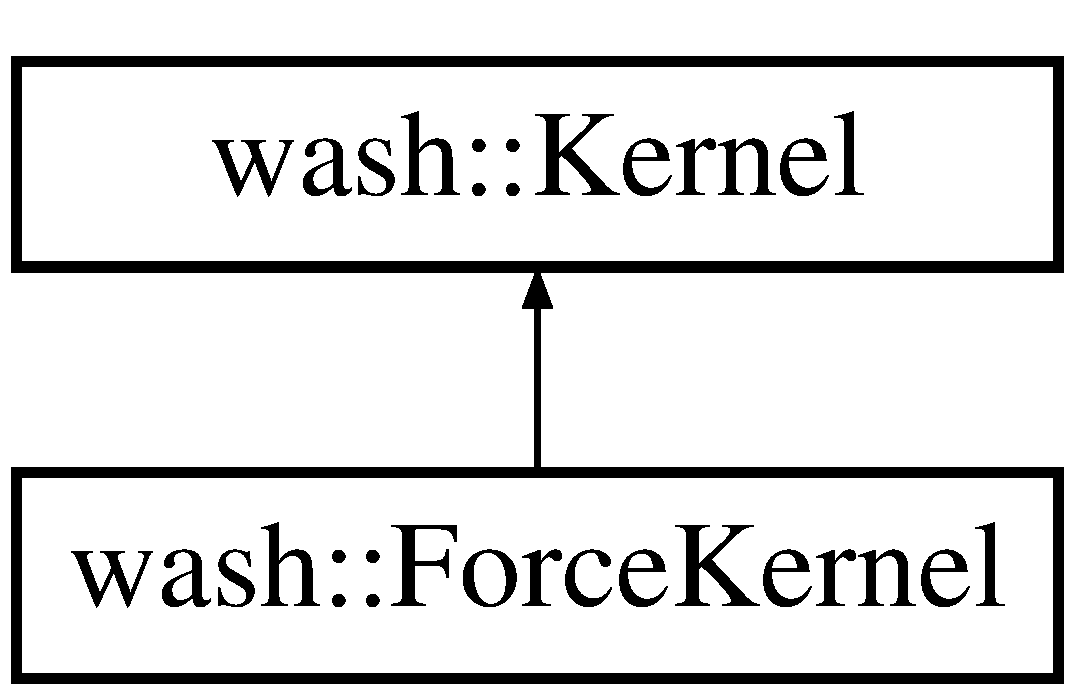
\includegraphics[height=2.000000cm]{classwash_1_1ForceKernel}
\end{center}
\end{figure}
\subsection*{Public Member Functions}
\begin{DoxyCompactItemize}
\item 
\mbox{\hyperlink{classwash_1_1ForceKernel_a5dd87d8036d74c210c51fb6aa97a3de8}{Force\+Kernel}} (const \mbox{\hyperlink{namespacewash_a3687ea698f8cb8c077d728e5d74de495}{Force\+FuncT}} func)
\item 
virtual void \mbox{\hyperlink{classwash_1_1ForceKernel_aa815514d4e9af5ebb056dbe8f1d5a720}{exec}} () const override
\end{DoxyCompactItemize}


\subsection{Detailed Description}
Force \mbox{\hyperlink{classwash_1_1Kernel}{Kernel}} Class. 

This kernel is used to update a force (or multiple forces) of a particle given its neighbours. 

\subsection{Constructor \& Destructor Documentation}
\mbox{\Hypertarget{classwash_1_1ForceKernel_a5dd87d8036d74c210c51fb6aa97a3de8}\label{classwash_1_1ForceKernel_a5dd87d8036d74c210c51fb6aa97a3de8}} 
\index{wash\+::\+Force\+Kernel@{wash\+::\+Force\+Kernel}!Force\+Kernel@{Force\+Kernel}}
\index{Force\+Kernel@{Force\+Kernel}!wash\+::\+Force\+Kernel@{wash\+::\+Force\+Kernel}}
\subsubsection{\texorpdfstring{Force\+Kernel()}{ForceKernel()}}
{\footnotesize\ttfamily wash\+::\+Force\+Kernel\+::\+Force\+Kernel (\begin{DoxyParamCaption}\item[{const \mbox{\hyperlink{namespacewash_a3687ea698f8cb8c077d728e5d74de495}{Force\+FuncT}}}]{func }\end{DoxyParamCaption})\hspace{0.3cm}{\ttfamily [inline]}}



\subsection{Member Function Documentation}
\mbox{\Hypertarget{classwash_1_1ForceKernel_aa815514d4e9af5ebb056dbe8f1d5a720}\label{classwash_1_1ForceKernel_aa815514d4e9af5ebb056dbe8f1d5a720}} 
\index{wash\+::\+Force\+Kernel@{wash\+::\+Force\+Kernel}!exec@{exec}}
\index{exec@{exec}!wash\+::\+Force\+Kernel@{wash\+::\+Force\+Kernel}}
\subsubsection{\texorpdfstring{exec()}{exec()}}
{\footnotesize\ttfamily void wash\+::\+Force\+Kernel\+::exec (\begin{DoxyParamCaption}{ }\end{DoxyParamCaption}) const\hspace{0.3cm}{\ttfamily [override]}, {\ttfamily [virtual]}}



Implements \mbox{\hyperlink{classwash_1_1Kernel_a0ec211840402ce975997b22136f16e39}{wash\+::\+Kernel}}.



The documentation for this class was generated from the following files\+:\begin{DoxyCompactItemize}
\item 
/dcs/20/u2002000/4th\+Year\+Project/wash/include/\mbox{\hyperlink{kernels_8hpp}{kernels.\+hpp}}\item 
/dcs/20/u2002000/4th\+Year\+Project/wash/src/impl/cstone/\mbox{\hyperlink{cstone_2kernels_8cpp}{kernels.\+cpp}}\end{DoxyCompactItemize}

\hypertarget{structImplementationFeatures}{}\section{Implementation\+Features Struct Reference}
\label{structImplementationFeatures}\index{Implementation\+Features@{Implementation\+Features}}


{\ttfamily \#include $<$common.\+hpp$>$}

\subsection*{Public Attributes}
\begin{DoxyCompactItemize}
\item 
uint8\+\_\+t \mbox{\hyperlink{structImplementationFeatures_a38b97cc0b2f3ea9db019845264fc060b}{openmp}}
\item 
uint8\+\_\+t \mbox{\hyperlink{structImplementationFeatures_a87a6ded1fc05396de42c11b17d41beca}{mpi}}
\item 
uint8\+\_\+t \mbox{\hyperlink{structImplementationFeatures_ac8156c774edb85175df22ff7f31dda44}{cuda}}
\item 
uint8\+\_\+t \mbox{\hyperlink{structImplementationFeatures_aaeaaaf6e801ac06863ba363591e938d7}{dim}}
\item 
std\+::string \mbox{\hyperlink{structImplementationFeatures_a7b7fb4c4e8fbf262d6697b8c25a17b5f}{name}}
\item 
std\+::string \mbox{\hyperlink{structImplementationFeatures_afe154ad26b28217f95c4cc74d7112049}{source\+\_\+dir}}
\end{DoxyCompactItemize}


\subsection{Member Data Documentation}
\mbox{\Hypertarget{structImplementationFeatures_ac8156c774edb85175df22ff7f31dda44}\label{structImplementationFeatures_ac8156c774edb85175df22ff7f31dda44}} 
\index{Implementation\+Features@{Implementation\+Features}!cuda@{cuda}}
\index{cuda@{cuda}!Implementation\+Features@{Implementation\+Features}}
\subsubsection{\texorpdfstring{cuda}{cuda}}
{\footnotesize\ttfamily uint8\+\_\+t Implementation\+Features\+::cuda}

\mbox{\Hypertarget{structImplementationFeatures_aaeaaaf6e801ac06863ba363591e938d7}\label{structImplementationFeatures_aaeaaaf6e801ac06863ba363591e938d7}} 
\index{Implementation\+Features@{Implementation\+Features}!dim@{dim}}
\index{dim@{dim}!Implementation\+Features@{Implementation\+Features}}
\subsubsection{\texorpdfstring{dim}{dim}}
{\footnotesize\ttfamily uint8\+\_\+t Implementation\+Features\+::dim}

\mbox{\Hypertarget{structImplementationFeatures_a87a6ded1fc05396de42c11b17d41beca}\label{structImplementationFeatures_a87a6ded1fc05396de42c11b17d41beca}} 
\index{Implementation\+Features@{Implementation\+Features}!mpi@{mpi}}
\index{mpi@{mpi}!Implementation\+Features@{Implementation\+Features}}
\subsubsection{\texorpdfstring{mpi}{mpi}}
{\footnotesize\ttfamily uint8\+\_\+t Implementation\+Features\+::mpi}

\mbox{\Hypertarget{structImplementationFeatures_a7b7fb4c4e8fbf262d6697b8c25a17b5f}\label{structImplementationFeatures_a7b7fb4c4e8fbf262d6697b8c25a17b5f}} 
\index{Implementation\+Features@{Implementation\+Features}!name@{name}}
\index{name@{name}!Implementation\+Features@{Implementation\+Features}}
\subsubsection{\texorpdfstring{name}{name}}
{\footnotesize\ttfamily std\+::string Implementation\+Features\+::name}

\mbox{\Hypertarget{structImplementationFeatures_a38b97cc0b2f3ea9db019845264fc060b}\label{structImplementationFeatures_a38b97cc0b2f3ea9db019845264fc060b}} 
\index{Implementation\+Features@{Implementation\+Features}!openmp@{openmp}}
\index{openmp@{openmp}!Implementation\+Features@{Implementation\+Features}}
\subsubsection{\texorpdfstring{openmp}{openmp}}
{\footnotesize\ttfamily uint8\+\_\+t Implementation\+Features\+::openmp}

\mbox{\Hypertarget{structImplementationFeatures_afe154ad26b28217f95c4cc74d7112049}\label{structImplementationFeatures_afe154ad26b28217f95c4cc74d7112049}} 
\index{Implementation\+Features@{Implementation\+Features}!source\+\_\+dir@{source\+\_\+dir}}
\index{source\+\_\+dir@{source\+\_\+dir}!Implementation\+Features@{Implementation\+Features}}
\subsubsection{\texorpdfstring{source\+\_\+dir}{source\_dir}}
{\footnotesize\ttfamily std\+::string Implementation\+Features\+::source\+\_\+dir}



The documentation for this struct was generated from the following file\+:\begin{DoxyCompactItemize}
\item 
/dcs/20/u2002000/4th\+Year\+Project/wash/src/ws2st/\mbox{\hyperlink{common_8hpp}{common.\+hpp}}\end{DoxyCompactItemize}

\hypertarget{classwash_1_1io_1_1IOManager}{}\section{wash\+:\+:io\+:\+:I\+O\+Manager Class Reference}
\label{classwash_1_1io_1_1IOManager}\index{wash\+::io\+::\+I\+O\+Manager@{wash\+::io\+::\+I\+O\+Manager}}


Manages the IO options for the simulation.  




{\ttfamily \#include $<$io.\+hpp$>$}

\subsection*{Public Types}
\begin{DoxyCompactItemize}
\item 
using \mbox{\hyperlink{classwash_1_1io_1_1IOManager_aeda8c39a8e3c748efd1b3e0f8ae823ee}{Writer\+FuncT}} = std\+::function$<$ int(const \mbox{\hyperlink{classwash_1_1io_1_1IOManager}{io\+::\+I\+O\+Manager}} \&, const \mbox{\hyperlink{structwash_1_1io_1_1SimulationData}{Simulation\+Data}} \&, const size\+\_\+t)$>$
\end{DoxyCompactItemize}
\subsection*{Public Member Functions}
\begin{DoxyCompactItemize}
\item 
\mbox{\hyperlink{classwash_1_1io_1_1IOManager_acea5f3f8a7f3e8eb1bfda9bc551b8435}{I\+O\+Manager}} (const std\+::string format, \mbox{\hyperlink{classwash_1_1io_1_1IOManager_aeda8c39a8e3c748efd1b3e0f8ae823ee}{Writer\+FuncT}} writer, const size\+\_\+t nth, const size\+\_\+t rank=0, const size\+\_\+t size=1, const bool \mbox{\hyperlink{namespacewash_a40aed5edcd0e0403841e3f83eaa41965}{timings}}=true)
\item 
\mbox{\hyperlink{classwash_1_1io_1_1IOManager_a736c595ca08833f2a4df8f0db90ceb28}{I\+O\+Manager}} (const std\+::string format, \mbox{\hyperlink{classwash_1_1io_1_1IOManager_aeda8c39a8e3c748efd1b3e0f8ae823ee}{Writer\+FuncT}} writer)
\item 
\mbox{\hyperlink{classwash_1_1io_1_1IOManager_af011701d8fed420a51bafe7fcf035774}{I\+O\+Manager}} (const std\+::string format, \mbox{\hyperlink{classwash_1_1io_1_1IOManager_aeda8c39a8e3c748efd1b3e0f8ae823ee}{Writer\+FuncT}} writer, const size\+\_\+t rank, const size\+\_\+t size)
\item 
\mbox{\hyperlink{classwash_1_1io_1_1IOManager_a2abea2ab5058a02b4bcf0876c0e179f7}{I\+O\+Manager}} ()
\item 
const std\+::string \mbox{\hyperlink{classwash_1_1io_1_1IOManager_aded7d1dbc7a4c2fc21e3a914ea0ea3b0}{get\+\_\+path}} () const
\item 
size\+\_\+t \mbox{\hyperlink{classwash_1_1io_1_1IOManager_ad290bc39e3c9ccafb070bf6ba75597b6}{get\+\_\+rank}} () const
\item 
size\+\_\+t \mbox{\hyperlink{classwash_1_1io_1_1IOManager_a01f3e40f12375f3128ad9b19f3ecda12}{get\+\_\+size}} () const
\item 
void \mbox{\hyperlink{classwash_1_1io_1_1IOManager_ab599141d728a1d6c09ce273a9e556eff}{set\+\_\+gather}} (bool value=true)
\item 
const std\+::string \& \mbox{\hyperlink{classwash_1_1io_1_1IOManager_ac0942e50fcd001ef853c8eb6b107e92d}{expand\+\_\+label}} (const std\+::string \&label) const
\begin{DoxyCompactList}\small\item\em Helper function to expand a label if an expansion exists. \end{DoxyCompactList}\item 
const \mbox{\hyperlink{structwash_1_1io_1_1SimulationData}{Simulation\+Data}} \mbox{\hyperlink{classwash_1_1io_1_1IOManager_acd4d5358ca4bb964926dfc080a72475c}{get\+\_\+simulation\+\_\+data}} ()
\begin{DoxyCompactList}\small\item\em Copies the simulation data at the current point of the simulation. \end{DoxyCompactList}\item 
void \mbox{\hyperlink{classwash_1_1io_1_1IOManager_ab4670696bfb277a364f6112fc6f0d051}{write\+\_\+iteration}} (const size\+\_\+t iteration)
\begin{DoxyCompactList}\small\item\em Dispatches an iteration call to the writer based on the iteration number. \end{DoxyCompactList}\item 
void \mbox{\hyperlink{classwash_1_1io_1_1IOManager_ab2397361f7dc4f7b54b559d332bafb11}{write\+\_\+timings}} (const std\+::string \&event\+\_\+name, const int tag, const int64\+\_\+t time\+\_\+taken) const
\begin{DoxyCompactList}\small\item\em Write a timing even out to a file. \end{DoxyCompactList}\item 
void \mbox{\hyperlink{classwash_1_1io_1_1IOManager_ae23d3d68354b0ba5b410992c60fe6762}{new\+\_\+timings}} ()
\begin{DoxyCompactList}\small\item\em Clear the timings output file. \end{DoxyCompactList}\end{DoxyCompactItemize}
\subsection*{Static Public Attributes}
\begin{DoxyCompactItemize}
\item 
static const std\+::unordered\+\_\+map$<$ std\+::string, std\+::string $>$ \mbox{\hyperlink{classwash_1_1io_1_1IOManager_ae2918fb006b6571b0eeceed90d2685b4}{label\+\_\+map}}
\end{DoxyCompactItemize}


\subsection{Detailed Description}
Manages the IO options for the simulation. 

\subsection{Member Typedef Documentation}
\mbox{\Hypertarget{classwash_1_1io_1_1IOManager_aeda8c39a8e3c748efd1b3e0f8ae823ee}\label{classwash_1_1io_1_1IOManager_aeda8c39a8e3c748efd1b3e0f8ae823ee}} 
\index{wash\+::io\+::\+I\+O\+Manager@{wash\+::io\+::\+I\+O\+Manager}!Writer\+FuncT@{Writer\+FuncT}}
\index{Writer\+FuncT@{Writer\+FuncT}!wash\+::io\+::\+I\+O\+Manager@{wash\+::io\+::\+I\+O\+Manager}}
\subsubsection{\texorpdfstring{Writer\+FuncT}{WriterFuncT}}
{\footnotesize\ttfamily using \mbox{\hyperlink{classwash_1_1io_1_1IOManager_aeda8c39a8e3c748efd1b3e0f8ae823ee}{wash\+::io\+::\+I\+O\+Manager\+::\+Writer\+FuncT}} =  std\+::function$<$int(const \mbox{\hyperlink{classwash_1_1io_1_1IOManager}{io\+::\+I\+O\+Manager}}\&, const \mbox{\hyperlink{structwash_1_1io_1_1SimulationData}{Simulation\+Data}}\&, const size\+\_\+t)$>$}



\subsection{Constructor \& Destructor Documentation}
\mbox{\Hypertarget{classwash_1_1io_1_1IOManager_acea5f3f8a7f3e8eb1bfda9bc551b8435}\label{classwash_1_1io_1_1IOManager_acea5f3f8a7f3e8eb1bfda9bc551b8435}} 
\index{wash\+::io\+::\+I\+O\+Manager@{wash\+::io\+::\+I\+O\+Manager}!I\+O\+Manager@{I\+O\+Manager}}
\index{I\+O\+Manager@{I\+O\+Manager}!wash\+::io\+::\+I\+O\+Manager@{wash\+::io\+::\+I\+O\+Manager}}
\subsubsection{\texorpdfstring{I\+O\+Manager()}{IOManager()}\hspace{0.1cm}{\footnotesize\ttfamily [1/4]}}
{\footnotesize\ttfamily wash\+::io\+::\+I\+O\+Manager\+::\+I\+O\+Manager (\begin{DoxyParamCaption}\item[{const std\+::string}]{format,  }\item[{\mbox{\hyperlink{classwash_1_1io_1_1IOManager_aeda8c39a8e3c748efd1b3e0f8ae823ee}{Writer\+FuncT}}}]{writer,  }\item[{const size\+\_\+t}]{nth,  }\item[{const size\+\_\+t}]{rank = {\ttfamily 0},  }\item[{const size\+\_\+t}]{size = {\ttfamily 1},  }\item[{const bool}]{timings = {\ttfamily true} }\end{DoxyParamCaption})\hspace{0.3cm}{\ttfamily [inline]}}

\mbox{\Hypertarget{classwash_1_1io_1_1IOManager_a736c595ca08833f2a4df8f0db90ceb28}\label{classwash_1_1io_1_1IOManager_a736c595ca08833f2a4df8f0db90ceb28}} 
\index{wash\+::io\+::\+I\+O\+Manager@{wash\+::io\+::\+I\+O\+Manager}!I\+O\+Manager@{I\+O\+Manager}}
\index{I\+O\+Manager@{I\+O\+Manager}!wash\+::io\+::\+I\+O\+Manager@{wash\+::io\+::\+I\+O\+Manager}}
\subsubsection{\texorpdfstring{I\+O\+Manager()}{IOManager()}\hspace{0.1cm}{\footnotesize\ttfamily [2/4]}}
{\footnotesize\ttfamily wash\+::io\+::\+I\+O\+Manager\+::\+I\+O\+Manager (\begin{DoxyParamCaption}\item[{const std\+::string}]{format,  }\item[{\mbox{\hyperlink{classwash_1_1io_1_1IOManager_aeda8c39a8e3c748efd1b3e0f8ae823ee}{Writer\+FuncT}}}]{writer }\end{DoxyParamCaption})\hspace{0.3cm}{\ttfamily [inline]}}

\mbox{\Hypertarget{classwash_1_1io_1_1IOManager_af011701d8fed420a51bafe7fcf035774}\label{classwash_1_1io_1_1IOManager_af011701d8fed420a51bafe7fcf035774}} 
\index{wash\+::io\+::\+I\+O\+Manager@{wash\+::io\+::\+I\+O\+Manager}!I\+O\+Manager@{I\+O\+Manager}}
\index{I\+O\+Manager@{I\+O\+Manager}!wash\+::io\+::\+I\+O\+Manager@{wash\+::io\+::\+I\+O\+Manager}}
\subsubsection{\texorpdfstring{I\+O\+Manager()}{IOManager()}\hspace{0.1cm}{\footnotesize\ttfamily [3/4]}}
{\footnotesize\ttfamily wash\+::io\+::\+I\+O\+Manager\+::\+I\+O\+Manager (\begin{DoxyParamCaption}\item[{const std\+::string}]{format,  }\item[{\mbox{\hyperlink{classwash_1_1io_1_1IOManager_aeda8c39a8e3c748efd1b3e0f8ae823ee}{Writer\+FuncT}}}]{writer,  }\item[{const size\+\_\+t}]{rank,  }\item[{const size\+\_\+t}]{size }\end{DoxyParamCaption})\hspace{0.3cm}{\ttfamily [inline]}}

\mbox{\Hypertarget{classwash_1_1io_1_1IOManager_a2abea2ab5058a02b4bcf0876c0e179f7}\label{classwash_1_1io_1_1IOManager_a2abea2ab5058a02b4bcf0876c0e179f7}} 
\index{wash\+::io\+::\+I\+O\+Manager@{wash\+::io\+::\+I\+O\+Manager}!I\+O\+Manager@{I\+O\+Manager}}
\index{I\+O\+Manager@{I\+O\+Manager}!wash\+::io\+::\+I\+O\+Manager@{wash\+::io\+::\+I\+O\+Manager}}
\subsubsection{\texorpdfstring{I\+O\+Manager()}{IOManager()}\hspace{0.1cm}{\footnotesize\ttfamily [4/4]}}
{\footnotesize\ttfamily wash\+::io\+::\+I\+O\+Manager\+::\+I\+O\+Manager (\begin{DoxyParamCaption}{ }\end{DoxyParamCaption})}



\subsection{Member Function Documentation}
\mbox{\Hypertarget{classwash_1_1io_1_1IOManager_ac0942e50fcd001ef853c8eb6b107e92d}\label{classwash_1_1io_1_1IOManager_ac0942e50fcd001ef853c8eb6b107e92d}} 
\index{wash\+::io\+::\+I\+O\+Manager@{wash\+::io\+::\+I\+O\+Manager}!expand\+\_\+label@{expand\+\_\+label}}
\index{expand\+\_\+label@{expand\+\_\+label}!wash\+::io\+::\+I\+O\+Manager@{wash\+::io\+::\+I\+O\+Manager}}
\subsubsection{\texorpdfstring{expand\+\_\+label()}{expand\_label()}}
{\footnotesize\ttfamily const std\+::string\& wash\+::io\+::\+I\+O\+Manager\+::expand\+\_\+label (\begin{DoxyParamCaption}\item[{const std\+::string \&}]{label }\end{DoxyParamCaption}) const\hspace{0.3cm}{\ttfamily [inline]}}



Helper function to expand a label if an expansion exists. 

\mbox{\Hypertarget{classwash_1_1io_1_1IOManager_aded7d1dbc7a4c2fc21e3a914ea0ea3b0}\label{classwash_1_1io_1_1IOManager_aded7d1dbc7a4c2fc21e3a914ea0ea3b0}} 
\index{wash\+::io\+::\+I\+O\+Manager@{wash\+::io\+::\+I\+O\+Manager}!get\+\_\+path@{get\+\_\+path}}
\index{get\+\_\+path@{get\+\_\+path}!wash\+::io\+::\+I\+O\+Manager@{wash\+::io\+::\+I\+O\+Manager}}
\subsubsection{\texorpdfstring{get\+\_\+path()}{get\_path()}}
{\footnotesize\ttfamily const std\+::string wash\+::io\+::\+I\+O\+Manager\+::get\+\_\+path (\begin{DoxyParamCaption}{ }\end{DoxyParamCaption}) const\hspace{0.3cm}{\ttfamily [inline]}}

\mbox{\Hypertarget{classwash_1_1io_1_1IOManager_ad290bc39e3c9ccafb070bf6ba75597b6}\label{classwash_1_1io_1_1IOManager_ad290bc39e3c9ccafb070bf6ba75597b6}} 
\index{wash\+::io\+::\+I\+O\+Manager@{wash\+::io\+::\+I\+O\+Manager}!get\+\_\+rank@{get\+\_\+rank}}
\index{get\+\_\+rank@{get\+\_\+rank}!wash\+::io\+::\+I\+O\+Manager@{wash\+::io\+::\+I\+O\+Manager}}
\subsubsection{\texorpdfstring{get\+\_\+rank()}{get\_rank()}}
{\footnotesize\ttfamily size\+\_\+t wash\+::io\+::\+I\+O\+Manager\+::get\+\_\+rank (\begin{DoxyParamCaption}{ }\end{DoxyParamCaption}) const\hspace{0.3cm}{\ttfamily [inline]}}

\mbox{\Hypertarget{classwash_1_1io_1_1IOManager_acd4d5358ca4bb964926dfc080a72475c}\label{classwash_1_1io_1_1IOManager_acd4d5358ca4bb964926dfc080a72475c}} 
\index{wash\+::io\+::\+I\+O\+Manager@{wash\+::io\+::\+I\+O\+Manager}!get\+\_\+simulation\+\_\+data@{get\+\_\+simulation\+\_\+data}}
\index{get\+\_\+simulation\+\_\+data@{get\+\_\+simulation\+\_\+data}!wash\+::io\+::\+I\+O\+Manager@{wash\+::io\+::\+I\+O\+Manager}}
\subsubsection{\texorpdfstring{get\+\_\+simulation\+\_\+data()}{get\_simulation\_data()}}
{\footnotesize\ttfamily const \mbox{\hyperlink{structwash_1_1io_1_1SimulationData}{Simulation\+Data}} wash\+::io\+::\+I\+O\+Manager\+::get\+\_\+simulation\+\_\+data (\begin{DoxyParamCaption}{ }\end{DoxyParamCaption})\hspace{0.3cm}{\ttfamily [inline]}}



Copies the simulation data at the current point of the simulation. 

If set to use a gather this will use M\+PI to gather from all processes

\begin{DoxyReturn}{Returns}
\mbox{\hyperlink{structwash_1_1io_1_1SimulationData}{Simulation\+Data}} The simulation data 
\end{DoxyReturn}
\mbox{\Hypertarget{classwash_1_1io_1_1IOManager_a01f3e40f12375f3128ad9b19f3ecda12}\label{classwash_1_1io_1_1IOManager_a01f3e40f12375f3128ad9b19f3ecda12}} 
\index{wash\+::io\+::\+I\+O\+Manager@{wash\+::io\+::\+I\+O\+Manager}!get\+\_\+size@{get\+\_\+size}}
\index{get\+\_\+size@{get\+\_\+size}!wash\+::io\+::\+I\+O\+Manager@{wash\+::io\+::\+I\+O\+Manager}}
\subsubsection{\texorpdfstring{get\+\_\+size()}{get\_size()}}
{\footnotesize\ttfamily size\+\_\+t wash\+::io\+::\+I\+O\+Manager\+::get\+\_\+size (\begin{DoxyParamCaption}{ }\end{DoxyParamCaption}) const\hspace{0.3cm}{\ttfamily [inline]}}

\mbox{\Hypertarget{classwash_1_1io_1_1IOManager_ae23d3d68354b0ba5b410992c60fe6762}\label{classwash_1_1io_1_1IOManager_ae23d3d68354b0ba5b410992c60fe6762}} 
\index{wash\+::io\+::\+I\+O\+Manager@{wash\+::io\+::\+I\+O\+Manager}!new\+\_\+timings@{new\+\_\+timings}}
\index{new\+\_\+timings@{new\+\_\+timings}!wash\+::io\+::\+I\+O\+Manager@{wash\+::io\+::\+I\+O\+Manager}}
\subsubsection{\texorpdfstring{new\+\_\+timings()}{new\_timings()}}
{\footnotesize\ttfamily void wash\+::io\+::\+I\+O\+Manager\+::new\+\_\+timings (\begin{DoxyParamCaption}{ }\end{DoxyParamCaption})\hspace{0.3cm}{\ttfamily [inline]}}



Clear the timings output file. 

\mbox{\Hypertarget{classwash_1_1io_1_1IOManager_ab599141d728a1d6c09ce273a9e556eff}\label{classwash_1_1io_1_1IOManager_ab599141d728a1d6c09ce273a9e556eff}} 
\index{wash\+::io\+::\+I\+O\+Manager@{wash\+::io\+::\+I\+O\+Manager}!set\+\_\+gather@{set\+\_\+gather}}
\index{set\+\_\+gather@{set\+\_\+gather}!wash\+::io\+::\+I\+O\+Manager@{wash\+::io\+::\+I\+O\+Manager}}
\subsubsection{\texorpdfstring{set\+\_\+gather()}{set\_gather()}}
{\footnotesize\ttfamily void wash\+::io\+::\+I\+O\+Manager\+::set\+\_\+gather (\begin{DoxyParamCaption}\item[{bool}]{value = {\ttfamily true} }\end{DoxyParamCaption})\hspace{0.3cm}{\ttfamily [inline]}}

\mbox{\Hypertarget{classwash_1_1io_1_1IOManager_ab4670696bfb277a364f6112fc6f0d051}\label{classwash_1_1io_1_1IOManager_ab4670696bfb277a364f6112fc6f0d051}} 
\index{wash\+::io\+::\+I\+O\+Manager@{wash\+::io\+::\+I\+O\+Manager}!write\+\_\+iteration@{write\+\_\+iteration}}
\index{write\+\_\+iteration@{write\+\_\+iteration}!wash\+::io\+::\+I\+O\+Manager@{wash\+::io\+::\+I\+O\+Manager}}
\subsubsection{\texorpdfstring{write\+\_\+iteration()}{write\_iteration()}}
{\footnotesize\ttfamily void wash\+::io\+::\+I\+O\+Manager\+::write\+\_\+iteration (\begin{DoxyParamCaption}\item[{const size\+\_\+t}]{iteration }\end{DoxyParamCaption})\hspace{0.3cm}{\ttfamily [inline]}}



Dispatches an iteration call to the writer based on the iteration number. 


\begin{DoxyParams}{Parameters}
{\em iteration} & \\
\hline
\end{DoxyParams}
\mbox{\Hypertarget{classwash_1_1io_1_1IOManager_ab2397361f7dc4f7b54b559d332bafb11}\label{classwash_1_1io_1_1IOManager_ab2397361f7dc4f7b54b559d332bafb11}} 
\index{wash\+::io\+::\+I\+O\+Manager@{wash\+::io\+::\+I\+O\+Manager}!write\+\_\+timings@{write\+\_\+timings}}
\index{write\+\_\+timings@{write\+\_\+timings}!wash\+::io\+::\+I\+O\+Manager@{wash\+::io\+::\+I\+O\+Manager}}
\subsubsection{\texorpdfstring{write\+\_\+timings()}{write\_timings()}}
{\footnotesize\ttfamily void wash\+::io\+::\+I\+O\+Manager\+::write\+\_\+timings (\begin{DoxyParamCaption}\item[{const std\+::string \&}]{event\+\_\+name,  }\item[{const int}]{tag,  }\item[{const int64\+\_\+t}]{time\+\_\+taken }\end{DoxyParamCaption}) const\hspace{0.3cm}{\ttfamily [inline]}}



Write a timing even out to a file. 


\begin{DoxyParams}{Parameters}
{\em event\+\_\+name} & \\
\hline
{\em time\+\_\+taken} & \\
\hline
\end{DoxyParams}


\subsection{Member Data Documentation}
\mbox{\Hypertarget{classwash_1_1io_1_1IOManager_ae2918fb006b6571b0eeceed90d2685b4}\label{classwash_1_1io_1_1IOManager_ae2918fb006b6571b0eeceed90d2685b4}} 
\index{wash\+::io\+::\+I\+O\+Manager@{wash\+::io\+::\+I\+O\+Manager}!label\+\_\+map@{label\+\_\+map}}
\index{label\+\_\+map@{label\+\_\+map}!wash\+::io\+::\+I\+O\+Manager@{wash\+::io\+::\+I\+O\+Manager}}
\subsubsection{\texorpdfstring{label\+\_\+map}{label\_map}}
{\footnotesize\ttfamily const std\+::unordered\+\_\+map$<$ std\+::string, std\+::string $>$ wash\+::io\+::\+I\+O\+Manager\+::label\+\_\+map\hspace{0.3cm}{\ttfamily [static]}}

{\bfseries Initial value\+:}
\begin{DoxyCode}
= \{ 
        \{\textcolor{stringliteral}{"id"}, \textcolor{stringliteral}{"ParticleIDs"}\},
        \{\textcolor{stringliteral}{"pos"}, \textcolor{stringliteral}{"Coordinates"}\},
        \{\textcolor{stringliteral}{"vel"}, \textcolor{stringliteral}{"Velocities"}\},
        \{\textcolor{stringliteral}{"acc"}, \textcolor{stringliteral}{"Acceleration"}\},
        \{\textcolor{stringliteral}{"rho"}, \textcolor{stringliteral}{"Density"}\},
        \{\textcolor{stringliteral}{"density"}, \textcolor{stringliteral}{"Density"}\},
        \{\textcolor{stringliteral}{"h"}, \textcolor{stringliteral}{"SmoothingLength"}\},
        \{\textcolor{stringliteral}{"smoothing\_length"}, \textcolor{stringliteral}{"SmoothingLength"}\},
        \{\textcolor{stringliteral}{"m"}, \textcolor{stringliteral}{"Masses"}\},
        \{\textcolor{stringliteral}{"mass"}, \textcolor{stringliteral}{"Masses"}\}
    \}
\end{DoxyCode}


The documentation for this class was generated from the following files\+:\begin{DoxyCompactItemize}
\item 
/dcs/20/u2002000/4th\+Year\+Project/wash/include/\mbox{\hyperlink{io_8hpp}{io.\+hpp}}\item 
/dcs/20/u2002000/4th\+Year\+Project/wash/src/io/\mbox{\hyperlink{io_2io_8cpp}{io.\+cpp}}\end{DoxyCompactItemize}

\hypertarget{classwash_1_1Kernel}{}\section{wash\+:\+:Kernel Class Reference}
\label{classwash_1_1Kernel}\index{wash\+::\+Kernel@{wash\+::\+Kernel}}


Parent \mbox{\hyperlink{classwash_1_1Kernel}{Kernel}} Class.  




{\ttfamily \#include $<$kernels.\+hpp$>$}

Inheritance diagram for wash\+:\+:Kernel\+:\begin{figure}[H]
\begin{center}
\leavevmode
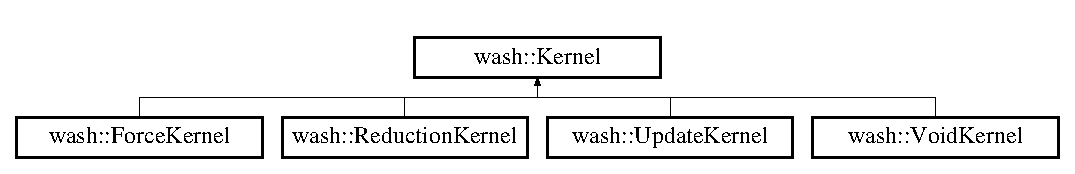
\includegraphics[height=1.891892cm]{classwash_1_1Kernel}
\end{center}
\end{figure}
\subsection*{Public Member Functions}
\begin{DoxyCompactItemize}
\item 
\mbox{\Hypertarget{classwash_1_1Kernel_a0ec211840402ce975997b22136f16e39}\label{classwash_1_1Kernel_a0ec211840402ce975997b22136f16e39}} 
virtual void {\bfseries exec} () const =0
\end{DoxyCompactItemize}


\subsection{Detailed Description}
Parent \mbox{\hyperlink{classwash_1_1Kernel}{Kernel}} Class. 

A \mbox{\hyperlink{classwash_1_1Kernel}{Kernel}} in Wa\+SH can take one of four forms, which all inherit from this class. 

The documentation for this class was generated from the following file\+:\begin{DoxyCompactItemize}
\item 
/dcs/20/u2002000/4th\+Year\+Project/wash/include/kernels.\+hpp\end{DoxyCompactItemize}

\hypertarget{structws2st_1_1KernelDependencies}{}\section{ws2st\+:\+:Kernel\+Dependencies Struct Reference}
\label{structws2st_1_1KernelDependencies}\index{ws2st\+::\+Kernel\+Dependencies@{ws2st\+::\+Kernel\+Dependencies}}


Struct to hold two vectors of dependencies (appropriately named)  




{\ttfamily \#include $<$common.\+hpp$>$}

\subsection*{Public Attributes}
\begin{DoxyCompactItemize}
\item 
\mbox{\Hypertarget{structws2st_1_1KernelDependencies_a4385ba2e56f0d9b63772480b2c3da15d}\label{structws2st_1_1KernelDependencies_a4385ba2e56f0d9b63772480b2c3da15d}} 
std\+::vector$<$ std\+::string $>$ {\bfseries reads\+\_\+from}
\item 
\mbox{\Hypertarget{structws2st_1_1KernelDependencies_a85a9ccadcb7d6912675a21cf500a4ef1}\label{structws2st_1_1KernelDependencies_a85a9ccadcb7d6912675a21cf500a4ef1}} 
std\+::vector$<$ std\+::string $>$ {\bfseries writes\+\_\+to}
\end{DoxyCompactItemize}


\subsection{Detailed Description}
Struct to hold two vectors of dependencies (appropriately named) 

The documentation for this struct was generated from the following file\+:\begin{DoxyCompactItemize}
\item 
/dcs/20/u2002000/4th\+Year\+Project/wash/src/ws2st/common.\+hpp\end{DoxyCompactItemize}

\hypertarget{classwash_1_1Particle}{}\section{wash\+:\+:Particle Class Reference}
\label{classwash_1_1Particle}\index{wash\+::\+Particle@{wash\+::\+Particle}}


{\ttfamily \#include $<$particle.\+hpp$>$}

\subsection*{Public Member Functions}
\begin{DoxyCompactItemize}
\item 
\mbox{\hyperlink{classwash_1_1Particle_a72131cdf3fdbcada383d81604fd49503}{Particle}} (const unsigned local\+\_\+idx)
\begin{DoxyCompactList}\small\item\em T\+O\+DO\+: see if this works if it\textquotesingle{}s a glocal spec defined flag rather than in just one file? \end{DoxyCompactList}\item 
unsigned \mbox{\hyperlink{classwash_1_1Particle_aef9f2814cc392598de7756e1046fea67}{get\+\_\+id}} () const
\begin{DoxyCompactList}\small\item\em Returns the global ID of the particle. \end{DoxyCompactList}\item 
double \mbox{\hyperlink{classwash_1_1Particle_a8c0ce3f48b189fd8550c3bfab17eec68}{get\+\_\+density}} () const
\item 
void \mbox{\hyperlink{classwash_1_1Particle_a6416678dd509c16c2933d315b6ae6156}{set\+\_\+density}} (const double \mbox{\hyperlink{3d__fluid__sim_2fluid__sim_8cpp_a140d94d7edb97c062961056d1926a2db}{density}})
\item 
double \mbox{\hyperlink{classwash_1_1Particle_a7d8d11b3e4855e66e62ee58b4270cdc1}{get\+\_\+mass}} () const
\item 
void \mbox{\hyperlink{classwash_1_1Particle_a9151ed34c880f63f062381076834223e}{set\+\_\+mass}} (const double mass)
\item 
double \mbox{\hyperlink{classwash_1_1Particle_aab02f56502c6521382cf7a7320abc341}{get\+\_\+smoothing\+\_\+length}} () const
\item 
void \mbox{\hyperlink{classwash_1_1Particle_a15892a4346c05de955f91087dc88786d}{set\+\_\+smoothing\+\_\+length}} (const double smoothing\+\_\+length)
\item 
\mbox{\hyperlink{namespacewash_ab2cbbc37941b733095c9225b49b4cad9}{Simulation\+VecT}} \mbox{\hyperlink{classwash_1_1Particle_a9d222d453d640cf629ee8dfbee6b43c2}{get\+\_\+pos}} () const
\item 
void \mbox{\hyperlink{classwash_1_1Particle_af06835533935c04e594c258a7dcdd1ef}{set\+\_\+pos}} (const \mbox{\hyperlink{namespacewash_ab2cbbc37941b733095c9225b49b4cad9}{Simulation\+VecT}} pos)
\item 
\mbox{\hyperlink{namespacewash_ab2cbbc37941b733095c9225b49b4cad9}{Simulation\+VecT}} \mbox{\hyperlink{classwash_1_1Particle_a890d0f1467225393e385872b0c98b974}{get\+\_\+vel}} () const
\item 
void \mbox{\hyperlink{classwash_1_1Particle_a4755365883cfd62117ebe74fe44d35e0}{set\+\_\+vel}} (const \mbox{\hyperlink{namespacewash_ab2cbbc37941b733095c9225b49b4cad9}{Simulation\+VecT}} vel)
\item 
\mbox{\hyperlink{namespacewash_ab2cbbc37941b733095c9225b49b4cad9}{Simulation\+VecT}} \mbox{\hyperlink{classwash_1_1Particle_afb8c9dce2692cdfab61a3a87fde50610}{get\+\_\+acc}} () const
\item 
void \mbox{\hyperlink{classwash_1_1Particle_a395e095de0b2af7dfc925bedef2090a1}{set\+\_\+acc}} (const \mbox{\hyperlink{namespacewash_ab2cbbc37941b733095c9225b49b4cad9}{Simulation\+VecT}} acc)
\item 
double \mbox{\hyperlink{classwash_1_1Particle_ab42a162b41a4e8cf6212bd9c43f3a0cf}{get\+\_\+force\+\_\+scalar}} (const std\+::string \&force) const
\item 
void \mbox{\hyperlink{classwash_1_1Particle_a2c3038c8eac34e371922bcf1ab79b8ca}{set\+\_\+force\+\_\+scalar}} (const std\+::string \&force, const double value)
\item 
\mbox{\hyperlink{namespacewash_ab2cbbc37941b733095c9225b49b4cad9}{Simulation\+VecT}} \mbox{\hyperlink{classwash_1_1Particle_a9c6ec5d5a7407897ecca00549bd05c01}{get\+\_\+force\+\_\+vector}} (const std\+::string \&force) const
\item 
void \mbox{\hyperlink{classwash_1_1Particle_a6960cdd169d1829a52e49cf835a8bfeb}{set\+\_\+force\+\_\+vector}} (const std\+::string \&force, const \mbox{\hyperlink{namespacewash_ab2cbbc37941b733095c9225b49b4cad9}{Simulation\+VecT}} value)
\item 
double \mbox{\hyperlink{classwash_1_1Particle_ab16021a2c003de07dc0a418ffc3d5eb7}{get\+\_\+vol}} () const
\item 
unsigned \mbox{\hyperlink{classwash_1_1Particle_a570fc3286ab83d081950a5fb3d548d92}{recalculate\+\_\+neighbors}} (unsigned max\+\_\+count) const
\item 
bool \mbox{\hyperlink{classwash_1_1Particle_a32369e6edba4277ebc71917a37c2503d}{operator==}} (const \mbox{\hyperlink{classwash_1_1Particle}{Particle}} \&other) const
\begin{DoxyCompactList}\small\item\em Compare particle equality by their I\+Ds. \end{DoxyCompactList}\item 
bool \mbox{\hyperlink{classwash_1_1Particle_a32f1334a8a0b273a57355956d7e9fe63}{operator!=}} (const \mbox{\hyperlink{classwash_1_1Particle}{Particle}} \&other) const
\begin{DoxyCompactList}\small\item\em Inverse of equality check. \end{DoxyCompactList}\item 
\mbox{\hyperlink{classwash_1_1Particle_a9ca04366cb7412e6aa5d1d89108a8520}{Particle}} (const \mbox{\hyperlink{classwash_1_1Particle}{Particle}} \&)=delete
\item 
\mbox{\hyperlink{classwash_1_1Particle}{Particle}} \& \mbox{\hyperlink{classwash_1_1Particle_a8ac44cec043e444a45ab189f666f9d4b}{operator=}} (const \mbox{\hyperlink{classwash_1_1Particle}{Particle}} \&)=delete
\end{DoxyCompactItemize}
\subsection*{Friends}
\begin{DoxyCompactItemize}
\item 
std\+::ostream \& \mbox{\hyperlink{classwash_1_1Particle_ad7d60c63b6d14d1d0d4fe42d4e9dc8bc}{operator$<$$<$}} (std\+::ostream \&os, const \mbox{\hyperlink{classwash_1_1Particle}{Particle}} \&p)
\end{DoxyCompactItemize}


\subsection{Constructor \& Destructor Documentation}
\mbox{\Hypertarget{classwash_1_1Particle_a72131cdf3fdbcada383d81604fd49503}\label{classwash_1_1Particle_a72131cdf3fdbcada383d81604fd49503}} 
\index{wash\+::\+Particle@{wash\+::\+Particle}!Particle@{Particle}}
\index{Particle@{Particle}!wash\+::\+Particle@{wash\+::\+Particle}}
\subsubsection{\texorpdfstring{Particle()}{Particle()}\hspace{0.1cm}{\footnotesize\ttfamily [1/2]}}
{\footnotesize\ttfamily wash\+::\+Particle\+::\+Particle (\begin{DoxyParamCaption}\item[{const unsigned}]{local\+\_\+idx }\end{DoxyParamCaption})}



T\+O\+DO\+: see if this works if it\textquotesingle{}s a glocal spec defined flag rather than in just one file? 

\mbox{\Hypertarget{classwash_1_1Particle_a9ca04366cb7412e6aa5d1d89108a8520}\label{classwash_1_1Particle_a9ca04366cb7412e6aa5d1d89108a8520}} 
\index{wash\+::\+Particle@{wash\+::\+Particle}!Particle@{Particle}}
\index{Particle@{Particle}!wash\+::\+Particle@{wash\+::\+Particle}}
\subsubsection{\texorpdfstring{Particle()}{Particle()}\hspace{0.1cm}{\footnotesize\ttfamily [2/2]}}
{\footnotesize\ttfamily wash\+::\+Particle\+::\+Particle (\begin{DoxyParamCaption}\item[{const \mbox{\hyperlink{classwash_1_1Particle}{Particle}} \&}]{ }\end{DoxyParamCaption})\hspace{0.3cm}{\ttfamily [delete]}}



\subsection{Member Function Documentation}
\mbox{\Hypertarget{classwash_1_1Particle_afb8c9dce2692cdfab61a3a87fde50610}\label{classwash_1_1Particle_afb8c9dce2692cdfab61a3a87fde50610}} 
\index{wash\+::\+Particle@{wash\+::\+Particle}!get\+\_\+acc@{get\+\_\+acc}}
\index{get\+\_\+acc@{get\+\_\+acc}!wash\+::\+Particle@{wash\+::\+Particle}}
\subsubsection{\texorpdfstring{get\+\_\+acc()}{get\_acc()}}
{\footnotesize\ttfamily \mbox{\hyperlink{namespacewash_ab2cbbc37941b733095c9225b49b4cad9}{Simulation\+VecT}} wash\+::\+Particle\+::get\+\_\+acc (\begin{DoxyParamCaption}{ }\end{DoxyParamCaption}) const}

\mbox{\Hypertarget{classwash_1_1Particle_a8c0ce3f48b189fd8550c3bfab17eec68}\label{classwash_1_1Particle_a8c0ce3f48b189fd8550c3bfab17eec68}} 
\index{wash\+::\+Particle@{wash\+::\+Particle}!get\+\_\+density@{get\+\_\+density}}
\index{get\+\_\+density@{get\+\_\+density}!wash\+::\+Particle@{wash\+::\+Particle}}
\subsubsection{\texorpdfstring{get\+\_\+density()}{get\_density()}}
{\footnotesize\ttfamily double wash\+::\+Particle\+::get\+\_\+density (\begin{DoxyParamCaption}{ }\end{DoxyParamCaption}) const}

\mbox{\Hypertarget{classwash_1_1Particle_ab42a162b41a4e8cf6212bd9c43f3a0cf}\label{classwash_1_1Particle_ab42a162b41a4e8cf6212bd9c43f3a0cf}} 
\index{wash\+::\+Particle@{wash\+::\+Particle}!get\+\_\+force\+\_\+scalar@{get\+\_\+force\+\_\+scalar}}
\index{get\+\_\+force\+\_\+scalar@{get\+\_\+force\+\_\+scalar}!wash\+::\+Particle@{wash\+::\+Particle}}
\subsubsection{\texorpdfstring{get\+\_\+force\+\_\+scalar()}{get\_force\_scalar()}}
{\footnotesize\ttfamily double wash\+::\+Particle\+::get\+\_\+force\+\_\+scalar (\begin{DoxyParamCaption}\item[{const std\+::string \&}]{force }\end{DoxyParamCaption}) const}

\mbox{\Hypertarget{classwash_1_1Particle_a9c6ec5d5a7407897ecca00549bd05c01}\label{classwash_1_1Particle_a9c6ec5d5a7407897ecca00549bd05c01}} 
\index{wash\+::\+Particle@{wash\+::\+Particle}!get\+\_\+force\+\_\+vector@{get\+\_\+force\+\_\+vector}}
\index{get\+\_\+force\+\_\+vector@{get\+\_\+force\+\_\+vector}!wash\+::\+Particle@{wash\+::\+Particle}}
\subsubsection{\texorpdfstring{get\+\_\+force\+\_\+vector()}{get\_force\_vector()}}
{\footnotesize\ttfamily \mbox{\hyperlink{namespacewash_ab2cbbc37941b733095c9225b49b4cad9}{Simulation\+VecT}} wash\+::\+Particle\+::get\+\_\+force\+\_\+vector (\begin{DoxyParamCaption}\item[{const std\+::string \&}]{force }\end{DoxyParamCaption}) const}

\mbox{\Hypertarget{classwash_1_1Particle_aef9f2814cc392598de7756e1046fea67}\label{classwash_1_1Particle_aef9f2814cc392598de7756e1046fea67}} 
\index{wash\+::\+Particle@{wash\+::\+Particle}!get\+\_\+id@{get\+\_\+id}}
\index{get\+\_\+id@{get\+\_\+id}!wash\+::\+Particle@{wash\+::\+Particle}}
\subsubsection{\texorpdfstring{get\+\_\+id()}{get\_id()}}
{\footnotesize\ttfamily unsigned wash\+::\+Particle\+::get\+\_\+id (\begin{DoxyParamCaption}{ }\end{DoxyParamCaption}) const}



Returns the global ID of the particle. 

\mbox{\Hypertarget{classwash_1_1Particle_a7d8d11b3e4855e66e62ee58b4270cdc1}\label{classwash_1_1Particle_a7d8d11b3e4855e66e62ee58b4270cdc1}} 
\index{wash\+::\+Particle@{wash\+::\+Particle}!get\+\_\+mass@{get\+\_\+mass}}
\index{get\+\_\+mass@{get\+\_\+mass}!wash\+::\+Particle@{wash\+::\+Particle}}
\subsubsection{\texorpdfstring{get\+\_\+mass()}{get\_mass()}}
{\footnotesize\ttfamily double wash\+::\+Particle\+::get\+\_\+mass (\begin{DoxyParamCaption}{ }\end{DoxyParamCaption}) const}

\mbox{\Hypertarget{classwash_1_1Particle_a9d222d453d640cf629ee8dfbee6b43c2}\label{classwash_1_1Particle_a9d222d453d640cf629ee8dfbee6b43c2}} 
\index{wash\+::\+Particle@{wash\+::\+Particle}!get\+\_\+pos@{get\+\_\+pos}}
\index{get\+\_\+pos@{get\+\_\+pos}!wash\+::\+Particle@{wash\+::\+Particle}}
\subsubsection{\texorpdfstring{get\+\_\+pos()}{get\_pos()}}
{\footnotesize\ttfamily \mbox{\hyperlink{namespacewash_ab2cbbc37941b733095c9225b49b4cad9}{Simulation\+VecT}} wash\+::\+Particle\+::get\+\_\+pos (\begin{DoxyParamCaption}{ }\end{DoxyParamCaption}) const}

\mbox{\Hypertarget{classwash_1_1Particle_aab02f56502c6521382cf7a7320abc341}\label{classwash_1_1Particle_aab02f56502c6521382cf7a7320abc341}} 
\index{wash\+::\+Particle@{wash\+::\+Particle}!get\+\_\+smoothing\+\_\+length@{get\+\_\+smoothing\+\_\+length}}
\index{get\+\_\+smoothing\+\_\+length@{get\+\_\+smoothing\+\_\+length}!wash\+::\+Particle@{wash\+::\+Particle}}
\subsubsection{\texorpdfstring{get\+\_\+smoothing\+\_\+length()}{get\_smoothing\_length()}}
{\footnotesize\ttfamily double wash\+::\+Particle\+::get\+\_\+smoothing\+\_\+length (\begin{DoxyParamCaption}{ }\end{DoxyParamCaption}) const}

\mbox{\Hypertarget{classwash_1_1Particle_a890d0f1467225393e385872b0c98b974}\label{classwash_1_1Particle_a890d0f1467225393e385872b0c98b974}} 
\index{wash\+::\+Particle@{wash\+::\+Particle}!get\+\_\+vel@{get\+\_\+vel}}
\index{get\+\_\+vel@{get\+\_\+vel}!wash\+::\+Particle@{wash\+::\+Particle}}
\subsubsection{\texorpdfstring{get\+\_\+vel()}{get\_vel()}}
{\footnotesize\ttfamily \mbox{\hyperlink{namespacewash_ab2cbbc37941b733095c9225b49b4cad9}{Simulation\+VecT}} wash\+::\+Particle\+::get\+\_\+vel (\begin{DoxyParamCaption}{ }\end{DoxyParamCaption}) const}

\mbox{\Hypertarget{classwash_1_1Particle_ab16021a2c003de07dc0a418ffc3d5eb7}\label{classwash_1_1Particle_ab16021a2c003de07dc0a418ffc3d5eb7}} 
\index{wash\+::\+Particle@{wash\+::\+Particle}!get\+\_\+vol@{get\+\_\+vol}}
\index{get\+\_\+vol@{get\+\_\+vol}!wash\+::\+Particle@{wash\+::\+Particle}}
\subsubsection{\texorpdfstring{get\+\_\+vol()}{get\_vol()}}
{\footnotesize\ttfamily double wash\+::\+Particle\+::get\+\_\+vol (\begin{DoxyParamCaption}{ }\end{DoxyParamCaption}) const}

\mbox{\Hypertarget{classwash_1_1Particle_a32f1334a8a0b273a57355956d7e9fe63}\label{classwash_1_1Particle_a32f1334a8a0b273a57355956d7e9fe63}} 
\index{wash\+::\+Particle@{wash\+::\+Particle}!operator"!=@{operator"!=}}
\index{operator"!=@{operator"!=}!wash\+::\+Particle@{wash\+::\+Particle}}
\subsubsection{\texorpdfstring{operator"!=()}{operator!=()}}
{\footnotesize\ttfamily bool wash\+::\+Particle\+::operator!= (\begin{DoxyParamCaption}\item[{const \mbox{\hyperlink{classwash_1_1Particle}{Particle}} \&}]{other }\end{DoxyParamCaption}) const}



Inverse of equality check. 


\begin{DoxyParams}{Parameters}
{\em other} & \\
\hline
\end{DoxyParams}
\begin{DoxyReturn}{Returns}
true 

false 
\end{DoxyReturn}
\mbox{\Hypertarget{classwash_1_1Particle_a8ac44cec043e444a45ab189f666f9d4b}\label{classwash_1_1Particle_a8ac44cec043e444a45ab189f666f9d4b}} 
\index{wash\+::\+Particle@{wash\+::\+Particle}!operator=@{operator=}}
\index{operator=@{operator=}!wash\+::\+Particle@{wash\+::\+Particle}}
\subsubsection{\texorpdfstring{operator=()}{operator=()}}
{\footnotesize\ttfamily \mbox{\hyperlink{classwash_1_1Particle}{Particle}}\& wash\+::\+Particle\+::operator= (\begin{DoxyParamCaption}\item[{const \mbox{\hyperlink{classwash_1_1Particle}{Particle}} \&}]{ }\end{DoxyParamCaption})\hspace{0.3cm}{\ttfamily [delete]}}

\mbox{\Hypertarget{classwash_1_1Particle_a32369e6edba4277ebc71917a37c2503d}\label{classwash_1_1Particle_a32369e6edba4277ebc71917a37c2503d}} 
\index{wash\+::\+Particle@{wash\+::\+Particle}!operator==@{operator==}}
\index{operator==@{operator==}!wash\+::\+Particle@{wash\+::\+Particle}}
\subsubsection{\texorpdfstring{operator==()}{operator==()}}
{\footnotesize\ttfamily bool wash\+::\+Particle\+::operator== (\begin{DoxyParamCaption}\item[{const \mbox{\hyperlink{classwash_1_1Particle}{Particle}} \&}]{other }\end{DoxyParamCaption}) const}



Compare particle equality by their I\+Ds. 


\begin{DoxyParams}{Parameters}
{\em other} & \\
\hline
\end{DoxyParams}
\begin{DoxyReturn}{Returns}
true ID\textquotesingle{}s equal 

false ID\textquotesingle{}s not equal 
\end{DoxyReturn}
\mbox{\Hypertarget{classwash_1_1Particle_a570fc3286ab83d081950a5fb3d548d92}\label{classwash_1_1Particle_a570fc3286ab83d081950a5fb3d548d92}} 
\index{wash\+::\+Particle@{wash\+::\+Particle}!recalculate\+\_\+neighbors@{recalculate\+\_\+neighbors}}
\index{recalculate\+\_\+neighbors@{recalculate\+\_\+neighbors}!wash\+::\+Particle@{wash\+::\+Particle}}
\subsubsection{\texorpdfstring{recalculate\+\_\+neighbors()}{recalculate\_neighbors()}}
{\footnotesize\ttfamily unsigned wash\+::\+Particle\+::recalculate\+\_\+neighbors (\begin{DoxyParamCaption}\item[{unsigned}]{max\+\_\+count }\end{DoxyParamCaption}) const}

\mbox{\Hypertarget{classwash_1_1Particle_a395e095de0b2af7dfc925bedef2090a1}\label{classwash_1_1Particle_a395e095de0b2af7dfc925bedef2090a1}} 
\index{wash\+::\+Particle@{wash\+::\+Particle}!set\+\_\+acc@{set\+\_\+acc}}
\index{set\+\_\+acc@{set\+\_\+acc}!wash\+::\+Particle@{wash\+::\+Particle}}
\subsubsection{\texorpdfstring{set\+\_\+acc()}{set\_acc()}}
{\footnotesize\ttfamily void wash\+::\+Particle\+::set\+\_\+acc (\begin{DoxyParamCaption}\item[{const \mbox{\hyperlink{namespacewash_ab2cbbc37941b733095c9225b49b4cad9}{Simulation\+VecT}}}]{acc }\end{DoxyParamCaption})}

\mbox{\Hypertarget{classwash_1_1Particle_a6416678dd509c16c2933d315b6ae6156}\label{classwash_1_1Particle_a6416678dd509c16c2933d315b6ae6156}} 
\index{wash\+::\+Particle@{wash\+::\+Particle}!set\+\_\+density@{set\+\_\+density}}
\index{set\+\_\+density@{set\+\_\+density}!wash\+::\+Particle@{wash\+::\+Particle}}
\subsubsection{\texorpdfstring{set\+\_\+density()}{set\_density()}}
{\footnotesize\ttfamily void wash\+::\+Particle\+::set\+\_\+density (\begin{DoxyParamCaption}\item[{const double}]{density }\end{DoxyParamCaption})}

\mbox{\Hypertarget{classwash_1_1Particle_a2c3038c8eac34e371922bcf1ab79b8ca}\label{classwash_1_1Particle_a2c3038c8eac34e371922bcf1ab79b8ca}} 
\index{wash\+::\+Particle@{wash\+::\+Particle}!set\+\_\+force\+\_\+scalar@{set\+\_\+force\+\_\+scalar}}
\index{set\+\_\+force\+\_\+scalar@{set\+\_\+force\+\_\+scalar}!wash\+::\+Particle@{wash\+::\+Particle}}
\subsubsection{\texorpdfstring{set\+\_\+force\+\_\+scalar()}{set\_force\_scalar()}}
{\footnotesize\ttfamily void wash\+::\+Particle\+::set\+\_\+force\+\_\+scalar (\begin{DoxyParamCaption}\item[{const std\+::string \&}]{force,  }\item[{const double}]{value }\end{DoxyParamCaption})}

\mbox{\Hypertarget{classwash_1_1Particle_a6960cdd169d1829a52e49cf835a8bfeb}\label{classwash_1_1Particle_a6960cdd169d1829a52e49cf835a8bfeb}} 
\index{wash\+::\+Particle@{wash\+::\+Particle}!set\+\_\+force\+\_\+vector@{set\+\_\+force\+\_\+vector}}
\index{set\+\_\+force\+\_\+vector@{set\+\_\+force\+\_\+vector}!wash\+::\+Particle@{wash\+::\+Particle}}
\subsubsection{\texorpdfstring{set\+\_\+force\+\_\+vector()}{set\_force\_vector()}}
{\footnotesize\ttfamily void wash\+::\+Particle\+::set\+\_\+force\+\_\+vector (\begin{DoxyParamCaption}\item[{const std\+::string \&}]{force,  }\item[{const \mbox{\hyperlink{namespacewash_ab2cbbc37941b733095c9225b49b4cad9}{Simulation\+VecT}}}]{value }\end{DoxyParamCaption})}

\mbox{\Hypertarget{classwash_1_1Particle_a9151ed34c880f63f062381076834223e}\label{classwash_1_1Particle_a9151ed34c880f63f062381076834223e}} 
\index{wash\+::\+Particle@{wash\+::\+Particle}!set\+\_\+mass@{set\+\_\+mass}}
\index{set\+\_\+mass@{set\+\_\+mass}!wash\+::\+Particle@{wash\+::\+Particle}}
\subsubsection{\texorpdfstring{set\+\_\+mass()}{set\_mass()}}
{\footnotesize\ttfamily void wash\+::\+Particle\+::set\+\_\+mass (\begin{DoxyParamCaption}\item[{const double}]{mass }\end{DoxyParamCaption})}

\mbox{\Hypertarget{classwash_1_1Particle_af06835533935c04e594c258a7dcdd1ef}\label{classwash_1_1Particle_af06835533935c04e594c258a7dcdd1ef}} 
\index{wash\+::\+Particle@{wash\+::\+Particle}!set\+\_\+pos@{set\+\_\+pos}}
\index{set\+\_\+pos@{set\+\_\+pos}!wash\+::\+Particle@{wash\+::\+Particle}}
\subsubsection{\texorpdfstring{set\+\_\+pos()}{set\_pos()}}
{\footnotesize\ttfamily void wash\+::\+Particle\+::set\+\_\+pos (\begin{DoxyParamCaption}\item[{const \mbox{\hyperlink{namespacewash_ab2cbbc37941b733095c9225b49b4cad9}{Simulation\+VecT}}}]{pos }\end{DoxyParamCaption})}

\mbox{\Hypertarget{classwash_1_1Particle_a15892a4346c05de955f91087dc88786d}\label{classwash_1_1Particle_a15892a4346c05de955f91087dc88786d}} 
\index{wash\+::\+Particle@{wash\+::\+Particle}!set\+\_\+smoothing\+\_\+length@{set\+\_\+smoothing\+\_\+length}}
\index{set\+\_\+smoothing\+\_\+length@{set\+\_\+smoothing\+\_\+length}!wash\+::\+Particle@{wash\+::\+Particle}}
\subsubsection{\texorpdfstring{set\+\_\+smoothing\+\_\+length()}{set\_smoothing\_length()}}
{\footnotesize\ttfamily void wash\+::\+Particle\+::set\+\_\+smoothing\+\_\+length (\begin{DoxyParamCaption}\item[{const double}]{smoothing\+\_\+length }\end{DoxyParamCaption})}

\mbox{\Hypertarget{classwash_1_1Particle_a4755365883cfd62117ebe74fe44d35e0}\label{classwash_1_1Particle_a4755365883cfd62117ebe74fe44d35e0}} 
\index{wash\+::\+Particle@{wash\+::\+Particle}!set\+\_\+vel@{set\+\_\+vel}}
\index{set\+\_\+vel@{set\+\_\+vel}!wash\+::\+Particle@{wash\+::\+Particle}}
\subsubsection{\texorpdfstring{set\+\_\+vel()}{set\_vel()}}
{\footnotesize\ttfamily void wash\+::\+Particle\+::set\+\_\+vel (\begin{DoxyParamCaption}\item[{const \mbox{\hyperlink{namespacewash_ab2cbbc37941b733095c9225b49b4cad9}{Simulation\+VecT}}}]{vel }\end{DoxyParamCaption})}



\subsection{Friends And Related Function Documentation}
\mbox{\Hypertarget{classwash_1_1Particle_ad7d60c63b6d14d1d0d4fe42d4e9dc8bc}\label{classwash_1_1Particle_ad7d60c63b6d14d1d0d4fe42d4e9dc8bc}} 
\index{wash\+::\+Particle@{wash\+::\+Particle}!operator$<$$<$@{operator$<$$<$}}
\index{operator$<$$<$@{operator$<$$<$}!wash\+::\+Particle@{wash\+::\+Particle}}
\subsubsection{\texorpdfstring{operator$<$$<$}{operator<<}}
{\footnotesize\ttfamily std\+::ostream\& operator$<$$<$ (\begin{DoxyParamCaption}\item[{std\+::ostream \&}]{os,  }\item[{const \mbox{\hyperlink{classwash_1_1Particle}{Particle}} \&}]{p }\end{DoxyParamCaption})\hspace{0.3cm}{\ttfamily [friend]}}



The documentation for this class was generated from the following files\+:\begin{DoxyCompactItemize}
\item 
/dcs/20/u2002000/4th\+Year\+Project/wash/include/\mbox{\hyperlink{particle_8hpp}{particle.\+hpp}}\item 
/dcs/20/u2002000/4th\+Year\+Project/wash/src/impl/cstone/\mbox{\hyperlink{cstone_2particle_8cpp}{particle.\+cpp}}\end{DoxyCompactItemize}

\hypertarget{classwash_1_1ReductionKernel}{}\section{wash\+:\+:Reduction\+Kernel Class Reference}
\label{classwash_1_1ReductionKernel}\index{wash\+::\+Reduction\+Kernel@{wash\+::\+Reduction\+Kernel}}
Inheritance diagram for wash\+:\+:Reduction\+Kernel\+:\begin{figure}[H]
\begin{center}
\leavevmode
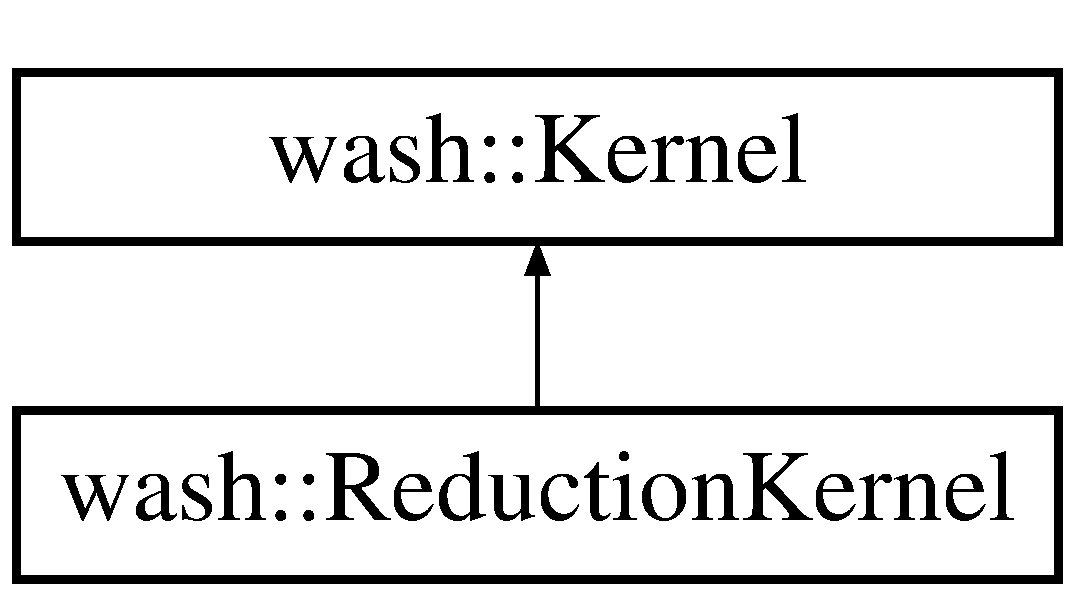
\includegraphics[height=2.000000cm]{classwash_1_1ReductionKernel}
\end{center}
\end{figure}
\subsection*{Public Member Functions}
\begin{DoxyCompactItemize}
\item 
\mbox{\Hypertarget{classwash_1_1ReductionKernel_ab916c2db7332203aed95dbd1adfbdd8e}\label{classwash_1_1ReductionKernel_ab916c2db7332203aed95dbd1adfbdd8e}} 
{\bfseries Reduction\+Kernel} (const Map\+FuncT map\+\_\+func, const Reduce\+FuncT reduce\+\_\+func, const double seed, const std\+::string variable)
\item 
\mbox{\Hypertarget{classwash_1_1ReductionKernel_a3ead90df8748700f40b2e6820e8e7e91}\label{classwash_1_1ReductionKernel_a3ead90df8748700f40b2e6820e8e7e91}} 
virtual void {\bfseries exec} () const override
\item 
\mbox{\Hypertarget{classwash_1_1ReductionKernel_ab916c2db7332203aed95dbd1adfbdd8e}\label{classwash_1_1ReductionKernel_ab916c2db7332203aed95dbd1adfbdd8e}} 
{\bfseries Reduction\+Kernel} (const Map\+FuncT map\+\_\+func, const Reduce\+FuncT reduce\+\_\+func, const double seed, const std\+::string variable)
\item 
\mbox{\Hypertarget{classwash_1_1ReductionKernel_aa06e992c0bc5d3e97fdf7553ad583bf3}\label{classwash_1_1ReductionKernel_aa06e992c0bc5d3e97fdf7553ad583bf3}} 
virtual void {\bfseries exec} () const override
\end{DoxyCompactItemize}


The documentation for this class was generated from the following files\+:\begin{DoxyCompactItemize}
\item 
/dcs/20/u2002000/4th\+Year\+Project/wash/src/wash/wash.\+hpp\item 
/dcs/20/u2002000/4th\+Year\+Project/wash/src/wash/wash.\+cpp\end{DoxyCompactItemize}

\hypertarget{classws2st_1_1refactor_1_1RefactoringToolConfiguration}{}\section{ws2st\+:\+:refactor\+:\+:Refactoring\+Tool\+Configuration Class Reference}
\label{classws2st_1_1refactor_1_1RefactoringToolConfiguration}\index{ws2st\+::refactor\+::\+Refactoring\+Tool\+Configuration@{ws2st\+::refactor\+::\+Refactoring\+Tool\+Configuration}}


We configure the whole tool by a series of refactoring passes.  




{\ttfamily \#include $<$refactor.\+hpp$>$}

\subsection*{Public Member Functions}
\begin{DoxyCompactItemize}
\item 
\mbox{\hyperlink{classws2st_1_1refactor_1_1RefactoringToolConfiguration_a6170e537d63c130d1224af83a5d0f41f}{Refactoring\+Tool\+Configuration}} (std\+::initializer\+\_\+list$<$ \mbox{\hyperlink{classws2st_1_1refactor_1_1RefactorPass}{Refactor\+Pass}} $>$ passes)
\item 
bool \mbox{\hyperlink{classws2st_1_1refactor_1_1RefactoringToolConfiguration_a7ff018cf2d0f2ec54274efcfa00df72f}{run}} (const \mbox{\hyperlink{structWashOptions}{Wash\+Options}} \&opts) const
\end{DoxyCompactItemize}


\subsection{Detailed Description}
We configure the whole tool by a series of refactoring passes. 


\begin{DoxyItemize}
\item each pass a stage where the tool runs through the source once 
\end{DoxyItemize}

\subsection{Constructor \& Destructor Documentation}
\mbox{\Hypertarget{classws2st_1_1refactor_1_1RefactoringToolConfiguration_a6170e537d63c130d1224af83a5d0f41f}\label{classws2st_1_1refactor_1_1RefactoringToolConfiguration_a6170e537d63c130d1224af83a5d0f41f}} 
\index{ws2st\+::refactor\+::\+Refactoring\+Tool\+Configuration@{ws2st\+::refactor\+::\+Refactoring\+Tool\+Configuration}!Refactoring\+Tool\+Configuration@{Refactoring\+Tool\+Configuration}}
\index{Refactoring\+Tool\+Configuration@{Refactoring\+Tool\+Configuration}!ws2st\+::refactor\+::\+Refactoring\+Tool\+Configuration@{ws2st\+::refactor\+::\+Refactoring\+Tool\+Configuration}}
\subsubsection{\texorpdfstring{Refactoring\+Tool\+Configuration()}{RefactoringToolConfiguration()}}
{\footnotesize\ttfamily ws2st\+::refactor\+::\+Refactoring\+Tool\+Configuration\+::\+Refactoring\+Tool\+Configuration (\begin{DoxyParamCaption}\item[{std\+::initializer\+\_\+list$<$ \mbox{\hyperlink{classws2st_1_1refactor_1_1RefactorPass}{Refactor\+Pass}} $>$}]{passes }\end{DoxyParamCaption})\hspace{0.3cm}{\ttfamily [inline]}}



\subsection{Member Function Documentation}
\mbox{\Hypertarget{classws2st_1_1refactor_1_1RefactoringToolConfiguration_a7ff018cf2d0f2ec54274efcfa00df72f}\label{classws2st_1_1refactor_1_1RefactoringToolConfiguration_a7ff018cf2d0f2ec54274efcfa00df72f}} 
\index{ws2st\+::refactor\+::\+Refactoring\+Tool\+Configuration@{ws2st\+::refactor\+::\+Refactoring\+Tool\+Configuration}!run@{run}}
\index{run@{run}!ws2st\+::refactor\+::\+Refactoring\+Tool\+Configuration@{ws2st\+::refactor\+::\+Refactoring\+Tool\+Configuration}}
\subsubsection{\texorpdfstring{run()}{run()}}
{\footnotesize\ttfamily bool ws2st\+::refactor\+::\+Refactoring\+Tool\+Configuration\+::run (\begin{DoxyParamCaption}\item[{const \mbox{\hyperlink{structWashOptions}{Wash\+Options}} \&}]{opts }\end{DoxyParamCaption}) const}



The documentation for this class was generated from the following files\+:\begin{DoxyCompactItemize}
\item 
/dcs/20/u2002000/4th\+Year\+Project/wash/src/ws2st/\mbox{\hyperlink{refactor_8hpp}{refactor.\+hpp}}\item 
/dcs/20/u2002000/4th\+Year\+Project/wash/src/ws2st/\mbox{\hyperlink{refactor_8cpp}{refactor.\+cpp}}\end{DoxyCompactItemize}

\hypertarget{classws2st_1_1refactor_1_1RefactorPass}{}\section{ws2st\+:\+:refactor\+:\+:Refactor\+Pass Class Reference}
\label{classws2st_1_1refactor_1_1RefactorPass}\index{ws2st\+::refactor\+::\+Refactor\+Pass@{ws2st\+::refactor\+::\+Refactor\+Pass}}


A pass of a refactoring tool over the source files running a series of actions defined.  




{\ttfamily \#include $<$refactor.\+hpp$>$}

\subsection*{Public Member Functions}
\begin{DoxyCompactItemize}
\item 
\mbox{\Hypertarget{classws2st_1_1refactor_1_1RefactorPass_a2e7cff9227709e40ebda3cb4acfc8fb4}\label{classws2st_1_1refactor_1_1RefactorPass_a2e7cff9227709e40ebda3cb4acfc8fb4}} 
{\bfseries Refactor\+Pass} (std\+::initializer\+\_\+list$<$ std\+::variant$<$ std\+::vector$<$ std\+::string $>$ $\ast$, \mbox{\hyperlink{classws2st_1_1refactor_1_1WashRefactoringAction}{Wash\+Refactoring\+Action}}, \mbox{\hyperlink{classws2st_1_1refactor_1_1WashComputationAction}{Wash\+Computation\+Action}} $>$$>$ actions)
\item 
\mbox{\Hypertarget{classws2st_1_1refactor_1_1RefactorPass_a349d409f7570c2516f690b8fe17ad20f}\label{classws2st_1_1refactor_1_1RefactorPass_a349d409f7570c2516f690b8fe17ad20f}} 
const std\+::vector$<$ \mbox{\hyperlink{classws2st_1_1refactor_1_1WashRefactoringAction}{Wash\+Refactoring\+Action}} $>$ \& {\bfseries actions} () const
\item 
\mbox{\Hypertarget{classws2st_1_1refactor_1_1RefactorPass_aa92ed5b7adb785f3cfb42f41b1a003e4}\label{classws2st_1_1refactor_1_1RefactorPass_aa92ed5b7adb785f3cfb42f41b1a003e4}} 
const std\+::vector$<$ \mbox{\hyperlink{classws2st_1_1refactor_1_1WashComputationAction}{Wash\+Computation\+Action}} $>$ \& {\bfseries computations} () const
\item 
\mbox{\Hypertarget{classws2st_1_1refactor_1_1RefactorPass_ac1c2e95b13d25ee91b5aa9c065296884}\label{classws2st_1_1refactor_1_1RefactorPass_ac1c2e95b13d25ee91b5aa9c065296884}} 
const std\+::vector$<$ std\+::string $>$ $\ast$ {\bfseries files} () const
\end{DoxyCompactItemize}


\subsection{Detailed Description}
A pass of a refactoring tool over the source files running a series of actions defined. 

The documentation for this class was generated from the following file\+:\begin{DoxyCompactItemize}
\item 
/dcs/20/u2002000/4th\+Year\+Project/wash/src/ws2st/\mbox{\hyperlink{refactor_8hpp}{refactor.\+hpp}}\end{DoxyCompactItemize}

\hypertarget{classSedovComputer}{}\section{Sedov\+Computer Class Reference}
\label{classSedovComputer}\index{Sedov\+Computer@{Sedov\+Computer}}
\subsection*{Static Public Member Functions}
\begin{DoxyCompactItemize}
\item 
\mbox{\Hypertarget{classSedovComputer_a5aa65182382334ed24bf803e60967795}\label{classSedovComputer_a5aa65182382334ed24bf803e60967795}} 
static double {\bfseries sedov\+Sol} (const size\+\_\+t dim, const double time, const double eblast, const double omega\+\_\+i, const double gamma\+\_\+i, const double rho0, const double u0, const double p0, const double vel0, const double cs0, const std\+::vector$<$ double $>$ \&r, std\+::vector$<$ double $>$ \&rho, std\+::vector$<$ double $>$ \&p, std\+::vector$<$ double $>$ \&u, std\+::vector$<$ double $>$ \&vel, std\+::vector$<$ double $>$ \&cs)
\end{DoxyCompactItemize}
\subsection*{Static Public Attributes}
\begin{DoxyCompactItemize}
\item 
\mbox{\Hypertarget{classSedovComputer_a3a79b1c2c435337f92488129f15ad323}\label{classSedovComputer_a3a79b1c2c435337f92488129f15ad323}} 
static double {\bfseries rho\+\_\+shock}
\item 
\mbox{\Hypertarget{classSedovComputer_aaca1a1a129526f6861d9c219a025ed56}\label{classSedovComputer_aaca1a1a129526f6861d9c219a025ed56}} 
static double {\bfseries p\+\_\+shock}
\item 
\mbox{\Hypertarget{classSedovComputer_ac8e574be46eb693b095e85c5d157bffb}\label{classSedovComputer_ac8e574be46eb693b095e85c5d157bffb}} 
static double {\bfseries vel\+\_\+shock}
\item 
\mbox{\Hypertarget{classSedovComputer_a597b5c8321e0737b514ddb121844053d}\label{classSedovComputer_a597b5c8321e0737b514ddb121844053d}} 
static double {\bfseries u\+\_\+shock}
\item 
\mbox{\Hypertarget{classSedovComputer_afd12699016e5eb9bc8c2c42ca4fb00bd}\label{classSedovComputer_afd12699016e5eb9bc8c2c42ca4fb00bd}} 
static double {\bfseries cs\+\_\+shock}
\end{DoxyCompactItemize}


The documentation for this class was generated from the following files\+:\begin{DoxyCompactItemize}
\item 
/dcs/20/u2002000/4th\+Year\+Project/wash/src/examples/sedov\+\_\+solution/\mbox{\hyperlink{sedov__computer_8hpp}{sedov\+\_\+computer.\+hpp}}\item 
/dcs/20/u2002000/4th\+Year\+Project/wash/src/examples/sedov\+\_\+solution/\mbox{\hyperlink{sedov__computer_8cpp}{sedov\+\_\+computer.\+cpp}}\end{DoxyCompactItemize}

\hypertarget{structwash_1_1io_1_1SimulationData}{}\section{wash\+:\+:io\+:\+:Simulation\+Data Struct Reference}
\label{structwash_1_1io_1_1SimulationData}\index{wash\+::io\+::\+Simulation\+Data@{wash\+::io\+::\+Simulation\+Data}}
\subsection*{Public Attributes}
\begin{DoxyCompactItemize}
\item 
\mbox{\Hypertarget{structwash_1_1io_1_1SimulationData_a21236f5ec63d5f10fedc79860baac63a}\label{structwash_1_1io_1_1SimulationData_a21236f5ec63d5f10fedc79860baac63a}} 
size\+\_\+t {\bfseries particle\+\_\+count}
\item 
\mbox{\Hypertarget{structwash_1_1io_1_1SimulationData_a6129996b88985d21217e8054e69cdf40}\label{structwash_1_1io_1_1SimulationData_a6129996b88985d21217e8054e69cdf40}} 
std\+::vector$<$ double $>$ {\bfseries data}
\item 
\mbox{\Hypertarget{structwash_1_1io_1_1SimulationData_af41f6f3caf54e0c7eee01b81c29f5617}\label{structwash_1_1io_1_1SimulationData_af41f6f3caf54e0c7eee01b81c29f5617}} 
std\+::vector$<$ std\+::string $>$ {\bfseries labels}
\item 
\mbox{\Hypertarget{structwash_1_1io_1_1SimulationData_a874b6512db1cf9a349da7a1b202f8dfe}\label{structwash_1_1io_1_1SimulationData_a874b6512db1cf9a349da7a1b202f8dfe}} 
std\+::vector$<$ unsigned short $>$ {\bfseries dim}
\end{DoxyCompactItemize}
\subsection*{Friends}
\begin{DoxyCompactItemize}
\item 
\mbox{\Hypertarget{structwash_1_1io_1_1SimulationData_ada32e2aed3a804ad52036cfe5ffe0540}\label{structwash_1_1io_1_1SimulationData_ada32e2aed3a804ad52036cfe5ffe0540}} 
std\+::ostream \& {\bfseries operator$<$$<$} (std\+::ostream \&os, const \mbox{\hyperlink{structwash_1_1io_1_1SimulationData}{Simulation\+Data}} \&data)
\end{DoxyCompactItemize}


The documentation for this struct was generated from the following file\+:\begin{DoxyCompactItemize}
\item 
/dcs/20/u2002000/4th\+Year\+Project/wash/include/io.\+hpp\end{DoxyCompactItemize}

\hypertarget{classwash_1_1UpdateKernel}{}\section{wash\+:\+:Update\+Kernel Class Reference}
\label{classwash_1_1UpdateKernel}\index{wash\+::\+Update\+Kernel@{wash\+::\+Update\+Kernel}}
Inheritance diagram for wash\+:\+:Update\+Kernel\+:\begin{figure}[H]
\begin{center}
\leavevmode
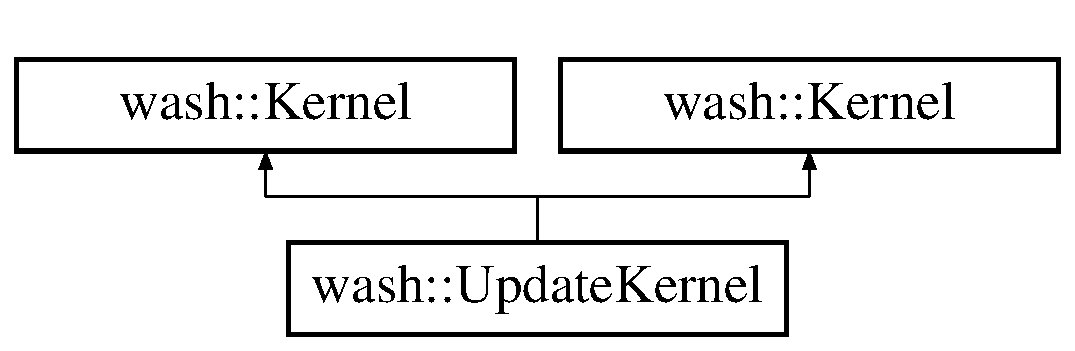
\includegraphics[height=2.000000cm]{classwash_1_1UpdateKernel}
\end{center}
\end{figure}
\subsection*{Public Member Functions}
\begin{DoxyCompactItemize}
\item 
\mbox{\Hypertarget{classwash_1_1UpdateKernel_a2cd95c4f9bcbceff9df7d094f7d7011f}\label{classwash_1_1UpdateKernel_a2cd95c4f9bcbceff9df7d094f7d7011f}} 
{\bfseries Update\+Kernel} (const Update\+FuncT func)
\item 
\mbox{\Hypertarget{classwash_1_1UpdateKernel_a72ec6b0ea453d97708f3fcfd98970366}\label{classwash_1_1UpdateKernel_a72ec6b0ea453d97708f3fcfd98970366}} 
virtual void {\bfseries exec} () const override
\item 
\mbox{\Hypertarget{classwash_1_1UpdateKernel_a2cd95c4f9bcbceff9df7d094f7d7011f}\label{classwash_1_1UpdateKernel_a2cd95c4f9bcbceff9df7d094f7d7011f}} 
{\bfseries Update\+Kernel} (const Update\+FuncT func)
\item 
\mbox{\Hypertarget{classwash_1_1UpdateKernel_a23c7bb181196e107afb1ca4ce9c79137}\label{classwash_1_1UpdateKernel_a23c7bb181196e107afb1ca4ce9c79137}} 
virtual void {\bfseries exec} () const override
\end{DoxyCompactItemize}


The documentation for this class was generated from the following files\+:\begin{DoxyCompactItemize}
\item 
/dcs/20/u2002000/4th\+Year\+Project/wash/src/wash/wash.\+hpp\item 
/dcs/20/u2002000/4th\+Year\+Project/wash/src/wash/wash.\+cpp\end{DoxyCompactItemize}

\hypertarget{classwash_1_1Vec}{}\section{wash\+:\+:Vec$<$ T, dim $>$ Class Template Reference}
\label{classwash_1_1Vec}\index{wash\+::\+Vec$<$ T, dim $>$@{wash\+::\+Vec$<$ T, dim $>$}}
\subsection*{Public Member Functions}
\begin{DoxyCompactItemize}
\item 
\mbox{\Hypertarget{classwash_1_1Vec_a6250ba5f027e9e0e974654136ea7e6ef}\label{classwash_1_1Vec_a6250ba5f027e9e0e974654136ea7e6ef}} 
{\bfseries Vec} (std\+::initializer\+\_\+list$<$ T $>$ l)
\item 
\mbox{\Hypertarget{classwash_1_1Vec_a5927d6caa8489a88b8470fe8bb8779d0}\label{classwash_1_1Vec_a5927d6caa8489a88b8470fe8bb8779d0}} 
T $\ast$ {\bfseries operator\mbox{[}$\,$\mbox{]}} (int i)
\item 
\mbox{\Hypertarget{classwash_1_1Vec_ad8a8863138b26c2b2eae41e11f40e78f}\label{classwash_1_1Vec_ad8a8863138b26c2b2eae41e11f40e78f}} 
\mbox{\hyperlink{classwash_1_1Vec}{Vec}}$<$ T, dim $>$ {\bfseries operator+} (T d)
\item 
\mbox{\Hypertarget{classwash_1_1Vec_a951a842c43b3cf99d60abfe73e53475c}\label{classwash_1_1Vec_a951a842c43b3cf99d60abfe73e53475c}} 
\mbox{\hyperlink{classwash_1_1Vec}{Vec}}$<$ T, dim $>$ {\bfseries operator+} (\mbox{\hyperlink{classwash_1_1Vec}{Vec}}$<$ T, dim $>$ v)
\item 
\mbox{\Hypertarget{classwash_1_1Vec_ac92d90da0a36cdd6b38a8a12e341fa84}\label{classwash_1_1Vec_ac92d90da0a36cdd6b38a8a12e341fa84}} 
void {\bfseries operator+=} (\mbox{\hyperlink{classwash_1_1Vec}{Vec}}$<$ T, dim $>$ v)
\item 
\mbox{\Hypertarget{classwash_1_1Vec_a83a86542f9afb7ea0b5b7b8ab72eb119}\label{classwash_1_1Vec_a83a86542f9afb7ea0b5b7b8ab72eb119}} 
\mbox{\hyperlink{classwash_1_1Vec}{Vec}}$<$ T, dim $>$ {\bfseries operator-\/} (\mbox{\hyperlink{classwash_1_1Vec}{Vec}}$<$ T, dim $>$ v) const
\item 
\mbox{\Hypertarget{classwash_1_1Vec_a972cde51776de1a9efec7ed6ea02f401}\label{classwash_1_1Vec_a972cde51776de1a9efec7ed6ea02f401}} 
\mbox{\hyperlink{classwash_1_1Vec}{Vec}}$<$ T, dim $>$ {\bfseries operator/} (T d)
\item 
\mbox{\Hypertarget{classwash_1_1Vec_a6fc9e30b352c72c7307bd28ee6c0aa72}\label{classwash_1_1Vec_a6fc9e30b352c72c7307bd28ee6c0aa72}} 
\mbox{\hyperlink{classwash_1_1Vec}{Vec}}$<$ T, dim $>$ {\bfseries operator$\ast$} (T d)
\item 
\mbox{\Hypertarget{classwash_1_1Vec_a41de499daf12160b2cf515ce0c9da70f}\label{classwash_1_1Vec_a41de499daf12160b2cf515ce0c9da70f}} 
T {\bfseries magnitude} ()
\item 
\mbox{\Hypertarget{classwash_1_1Vec_a1be26013b6d4f898b8504fc258043400}\label{classwash_1_1Vec_a1be26013b6d4f898b8504fc258043400}} 
T {\bfseries at} (const size\+\_\+t i) const
\item 
\mbox{\Hypertarget{classwash_1_1Vec_aae15a1a2cea7e883e53c2e7f6164710a}\label{classwash_1_1Vec_aae15a1a2cea7e883e53c2e7f6164710a}} 
\mbox{\hyperlink{classwash_1_1Vec}{Vec}}$<$ T, dim $>$ {\bfseries abs} () const
\end{DoxyCompactItemize}


The documentation for this class was generated from the following file\+:\begin{DoxyCompactItemize}
\item 
/dcs/20/u2002000/4th\+Year\+Project/wash/wash\+\_\+vector.\+hpp\end{DoxyCompactItemize}

\hypertarget{classwash_1_1VoidKernel}{}\section{wash\+:\+:Void\+Kernel Class Reference}
\label{classwash_1_1VoidKernel}\index{wash\+::\+Void\+Kernel@{wash\+::\+Void\+Kernel}}


Void \mbox{\hyperlink{classwash_1_1Kernel}{Kernel}} has no arguments/return.  




{\ttfamily \#include $<$kernels.\+hpp$>$}

Inheritance diagram for wash\+:\+:Void\+Kernel\+:\begin{figure}[H]
\begin{center}
\leavevmode
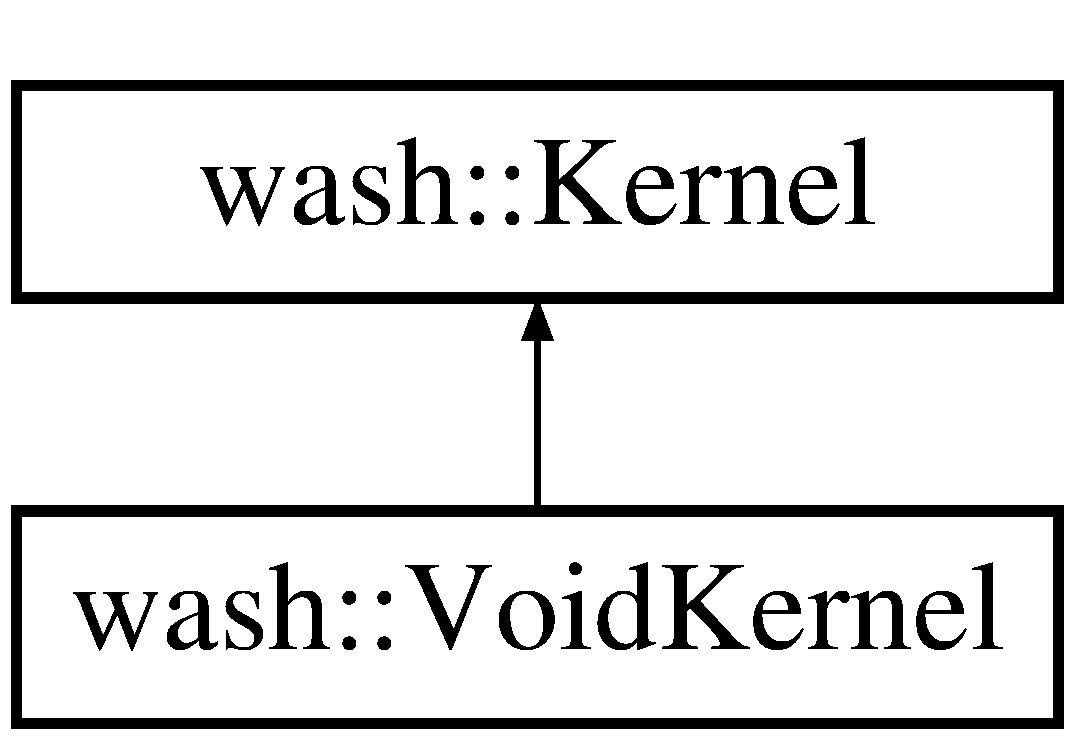
\includegraphics[height=2.000000cm]{classwash_1_1VoidKernel}
\end{center}
\end{figure}
\subsection*{Public Member Functions}
\begin{DoxyCompactItemize}
\item 
\mbox{\Hypertarget{classwash_1_1VoidKernel_abe7159c42c48bf15cf3d69dbf09388dc}\label{classwash_1_1VoidKernel_abe7159c42c48bf15cf3d69dbf09388dc}} 
{\bfseries Void\+Kernel} (const Void\+FuncT func)
\item 
\mbox{\Hypertarget{classwash_1_1VoidKernel_a2a271788509bac47a96dbbecd7fbe90e}\label{classwash_1_1VoidKernel_a2a271788509bac47a96dbbecd7fbe90e}} 
virtual void {\bfseries exec} () const override
\end{DoxyCompactItemize}


\subsection{Detailed Description}
Void \mbox{\hyperlink{classwash_1_1Kernel}{Kernel}} has no arguments/return. 

The documentation for this class was generated from the following files\+:\begin{DoxyCompactItemize}
\item 
/dcs/20/u2002000/4th\+Year\+Project/wash/include/kernels.\+hpp\item 
/dcs/20/u2002000/4th\+Year\+Project/wash/src/impl/cstone/kernels.\+cpp\end{DoxyCompactItemize}

\hypertarget{classws2st_1_1refactor_1_1WashComputationAction}{}\section{ws2st\+:\+:refactor\+:\+:Wash\+Computation\+Action Class Reference}
\label{classws2st_1_1refactor_1_1WashComputationAction}\index{ws2st\+::refactor\+::\+Wash\+Computation\+Action@{ws2st\+::refactor\+::\+Wash\+Computation\+Action}}


Define a function to be run at the end of the refactor pass. Computation Actions will be run in the order they\textquotesingle{}re defined, but will be run after all refactoring actions in the pass have completed.  




{\ttfamily \#include $<$refactor.\+hpp$>$}

\subsection*{Public Member Functions}
\begin{DoxyCompactItemize}
\item 
\mbox{\Hypertarget{classws2st_1_1refactor_1_1WashComputationAction_a5371af5f19e07759f4863e7b6011e787}\label{classws2st_1_1refactor_1_1WashComputationAction_a5371af5f19e07759f4863e7b6011e787}} 
{\bfseries Wash\+Computation\+Action} (Wash\+Compute\+Fn computefn\+\_\+ptr)
\item 
\mbox{\Hypertarget{classws2st_1_1refactor_1_1WashComputationAction_a195edd152f7fd88ca90d6dc7fb4897dc}\label{classws2st_1_1refactor_1_1WashComputationAction_a195edd152f7fd88ca90d6dc7fb4897dc}} 
Wash\+Compute\+Fn {\bfseries get\+Compute\+Fn} ()
\end{DoxyCompactItemize}


\subsection{Detailed Description}
Define a function to be run at the end of the refactor pass. Computation Actions will be run in the order they\textquotesingle{}re defined, but will be run after all refactoring actions in the pass have completed. 

The documentation for this class was generated from the following file\+:\begin{DoxyCompactItemize}
\item 
/dcs/20/u2002000/4th\+Year\+Project/wash/src/ws2st/\mbox{\hyperlink{refactor_8hpp}{refactor.\+hpp}}\end{DoxyCompactItemize}

\hypertarget{classws2st_1_1refactor_1_1WashMatchCallback}{}\section{ws2st\+:\+:refactor\+:\+:Wash\+Match\+Callback Class Reference}
\label{classws2st_1_1refactor_1_1WashMatchCallback}\index{ws2st\+::refactor\+::\+Wash\+Match\+Callback@{ws2st\+::refactor\+::\+Wash\+Match\+Callback}}


A specialised refactoring callback type for Wash using custom function pointers instead of subclassing tooling\+::\+Refactoring\+Callback and implementing ...\+::run a million times.  




{\ttfamily \#include $<$refactor.\+hpp$>$}

Inheritance diagram for ws2st\+:\+:refactor\+:\+:Wash\+Match\+Callback\+:\begin{figure}[H]
\begin{center}
\leavevmode
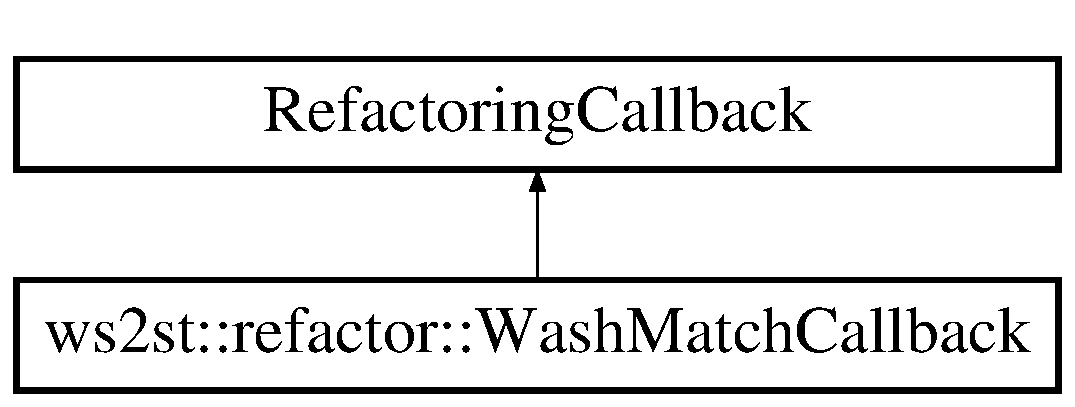
\includegraphics[height=2.000000cm]{classws2st_1_1refactor_1_1WashMatchCallback}
\end{center}
\end{figure}
\subsection*{Public Member Functions}
\begin{DoxyCompactItemize}
\item 
\mbox{\hyperlink{classws2st_1_1refactor_1_1WashMatchCallback_a92cc5cf8562d6d0df12547a5df116bec}{Wash\+Match\+Callback}} (\mbox{\hyperlink{namespacews2st_a682dfda40d8282c7e579a7b826a7d861}{Wash\+Callback\+Fn}} callback\+\_\+ptr)
\item 
virtual void \mbox{\hyperlink{classws2st_1_1refactor_1_1WashMatchCallback_a1712bb28c2728b43b5ca0f2d682382a6}{run}} (const Match\+Finder\+::\+Match\+Result \&Result)
\item 
\mbox{\hyperlink{namespacews2st_a682dfda40d8282c7e579a7b826a7d861}{Wash\+Callback\+Fn}} \mbox{\hyperlink{classws2st_1_1refactor_1_1WashMatchCallback_a91f255d66c7a62daa588b7f6910b5b50}{get\+Callback}} ()
\end{DoxyCompactItemize}
\subsection*{Friends}
\begin{DoxyCompactItemize}
\item 
std\+::ostream \& \mbox{\hyperlink{classws2st_1_1refactor_1_1WashMatchCallback_a0038f6cb22cb01fa32430f4857862513}{operator$<$$<$}} (std\+::ostream \&os, const \mbox{\hyperlink{classws2st_1_1refactor_1_1WashMatchCallback}{Wash\+Match\+Callback}} \&obj)
\end{DoxyCompactItemize}


\subsection{Detailed Description}
A specialised refactoring callback type for Wash using custom function pointers instead of subclassing tooling\+::\+Refactoring\+Callback and implementing ...\+::run a million times. 

\subsection{Constructor \& Destructor Documentation}
\mbox{\Hypertarget{classws2st_1_1refactor_1_1WashMatchCallback_a92cc5cf8562d6d0df12547a5df116bec}\label{classws2st_1_1refactor_1_1WashMatchCallback_a92cc5cf8562d6d0df12547a5df116bec}} 
\index{ws2st\+::refactor\+::\+Wash\+Match\+Callback@{ws2st\+::refactor\+::\+Wash\+Match\+Callback}!Wash\+Match\+Callback@{Wash\+Match\+Callback}}
\index{Wash\+Match\+Callback@{Wash\+Match\+Callback}!ws2st\+::refactor\+::\+Wash\+Match\+Callback@{ws2st\+::refactor\+::\+Wash\+Match\+Callback}}
\subsubsection{\texorpdfstring{Wash\+Match\+Callback()}{WashMatchCallback()}}
{\footnotesize\ttfamily ws2st\+::refactor\+::\+Wash\+Match\+Callback\+::\+Wash\+Match\+Callback (\begin{DoxyParamCaption}\item[{\mbox{\hyperlink{namespacews2st_a682dfda40d8282c7e579a7b826a7d861}{Wash\+Callback\+Fn}}}]{callback\+\_\+ptr }\end{DoxyParamCaption})\hspace{0.3cm}{\ttfamily [inline]}}



\subsection{Member Function Documentation}
\mbox{\Hypertarget{classws2st_1_1refactor_1_1WashMatchCallback_a91f255d66c7a62daa588b7f6910b5b50}\label{classws2st_1_1refactor_1_1WashMatchCallback_a91f255d66c7a62daa588b7f6910b5b50}} 
\index{ws2st\+::refactor\+::\+Wash\+Match\+Callback@{ws2st\+::refactor\+::\+Wash\+Match\+Callback}!get\+Callback@{get\+Callback}}
\index{get\+Callback@{get\+Callback}!ws2st\+::refactor\+::\+Wash\+Match\+Callback@{ws2st\+::refactor\+::\+Wash\+Match\+Callback}}
\subsubsection{\texorpdfstring{get\+Callback()}{getCallback()}}
{\footnotesize\ttfamily \mbox{\hyperlink{namespacews2st_a682dfda40d8282c7e579a7b826a7d861}{Wash\+Callback\+Fn}} ws2st\+::refactor\+::\+Wash\+Match\+Callback\+::get\+Callback (\begin{DoxyParamCaption}{ }\end{DoxyParamCaption})\hspace{0.3cm}{\ttfamily [inline]}}

\mbox{\Hypertarget{classws2st_1_1refactor_1_1WashMatchCallback_a1712bb28c2728b43b5ca0f2d682382a6}\label{classws2st_1_1refactor_1_1WashMatchCallback_a1712bb28c2728b43b5ca0f2d682382a6}} 
\index{ws2st\+::refactor\+::\+Wash\+Match\+Callback@{ws2st\+::refactor\+::\+Wash\+Match\+Callback}!run@{run}}
\index{run@{run}!ws2st\+::refactor\+::\+Wash\+Match\+Callback@{ws2st\+::refactor\+::\+Wash\+Match\+Callback}}
\subsubsection{\texorpdfstring{run()}{run()}}
{\footnotesize\ttfamily virtual void ws2st\+::refactor\+::\+Wash\+Match\+Callback\+::run (\begin{DoxyParamCaption}\item[{const Match\+Finder\+::\+Match\+Result \&}]{Result }\end{DoxyParamCaption})\hspace{0.3cm}{\ttfamily [inline]}, {\ttfamily [virtual]}}



\subsection{Friends And Related Function Documentation}
\mbox{\Hypertarget{classws2st_1_1refactor_1_1WashMatchCallback_a0038f6cb22cb01fa32430f4857862513}\label{classws2st_1_1refactor_1_1WashMatchCallback_a0038f6cb22cb01fa32430f4857862513}} 
\index{ws2st\+::refactor\+::\+Wash\+Match\+Callback@{ws2st\+::refactor\+::\+Wash\+Match\+Callback}!operator$<$$<$@{operator$<$$<$}}
\index{operator$<$$<$@{operator$<$$<$}!ws2st\+::refactor\+::\+Wash\+Match\+Callback@{ws2st\+::refactor\+::\+Wash\+Match\+Callback}}
\subsubsection{\texorpdfstring{operator$<$$<$}{operator<<}}
{\footnotesize\ttfamily std\+::ostream\& operator$<$$<$ (\begin{DoxyParamCaption}\item[{std\+::ostream \&}]{os,  }\item[{const \mbox{\hyperlink{classws2st_1_1refactor_1_1WashMatchCallback}{Wash\+Match\+Callback}} \&}]{obj }\end{DoxyParamCaption})\hspace{0.3cm}{\ttfamily [friend]}}



The documentation for this class was generated from the following file\+:\begin{DoxyCompactItemize}
\item 
/dcs/20/u2002000/4th\+Year\+Project/wash/src/ws2st/\mbox{\hyperlink{refactor_8hpp}{refactor.\+hpp}}\end{DoxyCompactItemize}

\hypertarget{structWashOptions}{}\section{Wash\+Options Struct Reference}
\label{structWashOptions}\index{Wash\+Options@{Wash\+Options}}


Options about how the Wash analysis will behave.  




{\ttfamily \#include $<$common.\+hpp$>$}

\subsection*{Public Attributes}
\begin{DoxyCompactItemize}
\item 
\mbox{\hyperlink{common_8hpp_aad9d1428f17c06ff77ef15dea22624dc}{Implementations}} \mbox{\hyperlink{structWashOptions_a44a1b923dc5034a3bf45dee2f54623ca}{impl}}
\item 
bool \mbox{\hyperlink{structWashOptions_a50d97883a6c0eaf8bafda97f5bad2a1e}{openmp}}
\item 
bool \mbox{\hyperlink{structWashOptions_a9ec267278d89d04982e3d70e877d5c67}{mpi}}
\item 
bool \mbox{\hyperlink{structWashOptions_a31ed802896363b97ac1f5199a6940df9}{hdf5}}
\item 
bool \mbox{\hyperlink{structWashOptions_a5bc365ad8fc0544864d15709b6808843}{debug}}
\item 
uint8\+\_\+t \mbox{\hyperlink{structWashOptions_a0caa33c545fc380c4104ca90f6462dfb}{dim}}
\item 
std\+::string \mbox{\hyperlink{structWashOptions_a4b43b8f0700908a6975a367d2cb9d567}{input\+\_\+path}}
\item 
std\+::string \mbox{\hyperlink{structWashOptions_a091c31f0eee54c7b079268f7a1001547}{output\+\_\+name}}
\item 
std\+::string \mbox{\hyperlink{structWashOptions_a27f59d7e66cdf80f0fe5cc5e699b0953}{temp\+\_\+path}}
\item 
std\+::vector$<$ std\+::string $>$ \mbox{\hyperlink{structWashOptions_abc32ad74441fbc82069b4addc130d4cd}{args}}
\end{DoxyCompactItemize}


\subsection{Detailed Description}
Options about how the Wash analysis will behave. 

Whether to enable certain features via flags in the compiler analysis and then again in the final compilation stages.

T\+O\+DO\+: If multiple options are enabled which are contradictory, then we should generate multiple output binaries at the end. 

\subsection{Member Data Documentation}
\mbox{\Hypertarget{structWashOptions_abc32ad74441fbc82069b4addc130d4cd}\label{structWashOptions_abc32ad74441fbc82069b4addc130d4cd}} 
\index{Wash\+Options@{Wash\+Options}!args@{args}}
\index{args@{args}!Wash\+Options@{Wash\+Options}}
\subsubsection{\texorpdfstring{args}{args}}
{\footnotesize\ttfamily std\+::vector$<$std\+::string$>$ Wash\+Options\+::args}

\mbox{\Hypertarget{structWashOptions_a5bc365ad8fc0544864d15709b6808843}\label{structWashOptions_a5bc365ad8fc0544864d15709b6808843}} 
\index{Wash\+Options@{Wash\+Options}!debug@{debug}}
\index{debug@{debug}!Wash\+Options@{Wash\+Options}}
\subsubsection{\texorpdfstring{debug}{debug}}
{\footnotesize\ttfamily bool Wash\+Options\+::debug}

\mbox{\Hypertarget{structWashOptions_a0caa33c545fc380c4104ca90f6462dfb}\label{structWashOptions_a0caa33c545fc380c4104ca90f6462dfb}} 
\index{Wash\+Options@{Wash\+Options}!dim@{dim}}
\index{dim@{dim}!Wash\+Options@{Wash\+Options}}
\subsubsection{\texorpdfstring{dim}{dim}}
{\footnotesize\ttfamily uint8\+\_\+t Wash\+Options\+::dim}

\mbox{\Hypertarget{structWashOptions_a31ed802896363b97ac1f5199a6940df9}\label{structWashOptions_a31ed802896363b97ac1f5199a6940df9}} 
\index{Wash\+Options@{Wash\+Options}!hdf5@{hdf5}}
\index{hdf5@{hdf5}!Wash\+Options@{Wash\+Options}}
\subsubsection{\texorpdfstring{hdf5}{hdf5}}
{\footnotesize\ttfamily bool Wash\+Options\+::hdf5}

\mbox{\Hypertarget{structWashOptions_a44a1b923dc5034a3bf45dee2f54623ca}\label{structWashOptions_a44a1b923dc5034a3bf45dee2f54623ca}} 
\index{Wash\+Options@{Wash\+Options}!impl@{impl}}
\index{impl@{impl}!Wash\+Options@{Wash\+Options}}
\subsubsection{\texorpdfstring{impl}{impl}}
{\footnotesize\ttfamily \mbox{\hyperlink{common_8hpp_aad9d1428f17c06ff77ef15dea22624dc}{Implementations}} Wash\+Options\+::impl}

\mbox{\Hypertarget{structWashOptions_a4b43b8f0700908a6975a367d2cb9d567}\label{structWashOptions_a4b43b8f0700908a6975a367d2cb9d567}} 
\index{Wash\+Options@{Wash\+Options}!input\+\_\+path@{input\+\_\+path}}
\index{input\+\_\+path@{input\+\_\+path}!Wash\+Options@{Wash\+Options}}
\subsubsection{\texorpdfstring{input\+\_\+path}{input\_path}}
{\footnotesize\ttfamily std\+::string Wash\+Options\+::input\+\_\+path}

\mbox{\Hypertarget{structWashOptions_a9ec267278d89d04982e3d70e877d5c67}\label{structWashOptions_a9ec267278d89d04982e3d70e877d5c67}} 
\index{Wash\+Options@{Wash\+Options}!mpi@{mpi}}
\index{mpi@{mpi}!Wash\+Options@{Wash\+Options}}
\subsubsection{\texorpdfstring{mpi}{mpi}}
{\footnotesize\ttfamily bool Wash\+Options\+::mpi}

\mbox{\Hypertarget{structWashOptions_a50d97883a6c0eaf8bafda97f5bad2a1e}\label{structWashOptions_a50d97883a6c0eaf8bafda97f5bad2a1e}} 
\index{Wash\+Options@{Wash\+Options}!openmp@{openmp}}
\index{openmp@{openmp}!Wash\+Options@{Wash\+Options}}
\subsubsection{\texorpdfstring{openmp}{openmp}}
{\footnotesize\ttfamily bool Wash\+Options\+::openmp}

\mbox{\Hypertarget{structWashOptions_a091c31f0eee54c7b079268f7a1001547}\label{structWashOptions_a091c31f0eee54c7b079268f7a1001547}} 
\index{Wash\+Options@{Wash\+Options}!output\+\_\+name@{output\+\_\+name}}
\index{output\+\_\+name@{output\+\_\+name}!Wash\+Options@{Wash\+Options}}
\subsubsection{\texorpdfstring{output\+\_\+name}{output\_name}}
{\footnotesize\ttfamily std\+::string Wash\+Options\+::output\+\_\+name}

\mbox{\Hypertarget{structWashOptions_a27f59d7e66cdf80f0fe5cc5e699b0953}\label{structWashOptions_a27f59d7e66cdf80f0fe5cc5e699b0953}} 
\index{Wash\+Options@{Wash\+Options}!temp\+\_\+path@{temp\+\_\+path}}
\index{temp\+\_\+path@{temp\+\_\+path}!Wash\+Options@{Wash\+Options}}
\subsubsection{\texorpdfstring{temp\+\_\+path}{temp\_path}}
{\footnotesize\ttfamily std\+::string Wash\+Options\+::temp\+\_\+path}



The documentation for this struct was generated from the following file\+:\begin{DoxyCompactItemize}
\item 
/dcs/20/u2002000/4th\+Year\+Project/wash/src/ws2st/\mbox{\hyperlink{common_8hpp}{common.\+hpp}}\end{DoxyCompactItemize}

\hypertarget{structws2st_1_1WashProgramMeta}{}\section{ws2st\+:\+:Wash\+Program\+Meta Struct Reference}
\label{structws2st_1_1WashProgramMeta}\index{ws2st\+::\+Wash\+Program\+Meta@{ws2st\+::\+Wash\+Program\+Meta}}


Meta information about the simulation which is defined globally and can be read/written to by the callback functions.  




{\ttfamily \#include $<$common.\+hpp$>$}

\subsection*{Public Attributes}
\begin{DoxyCompactItemize}
\item 
std\+::vector$<$ std\+::string $>$ \mbox{\hyperlink{structws2st_1_1WashProgramMeta_a71dfe0ec3a593707b26a3387d6ffe097}{scalar\+\_\+force\+\_\+list}}
\item 
std\+::vector$<$ std\+::string $>$ \mbox{\hyperlink{structws2st_1_1WashProgramMeta_a4b2ccb325270ac70589972a556b704b5}{vector\+\_\+force\+\_\+list}}
\item 
std\+::unordered\+\_\+map$<$ std\+::string, Full\+Source\+Loc $>$ \mbox{\hyperlink{structws2st_1_1WashProgramMeta_a2769172e26989f7d8759906460bbd43c}{force\+\_\+meta}}
\item 
std\+::vector$<$ std\+::pair$<$ std\+::string, std\+::string $>$ $>$ \mbox{\hyperlink{structws2st_1_1WashProgramMeta_ac42b81ba6becd8cba9834dc903704e5c}{variable\+\_\+list}}
\item 
int \mbox{\hyperlink{structws2st_1_1WashProgramMeta_a3a521dc326a6070a0af9c4bbec3913f4}{simulation\+\_\+dimension}}
\item 
std\+::vector$<$ std\+::string $>$ \mbox{\hyperlink{structws2st_1_1WashProgramMeta_ae19b95e2db30a6d8b366b1c9965b4806}{kernels\+\_\+list}}
\item 
std\+::vector$<$ std\+::string $>$ \mbox{\hyperlink{structws2st_1_1WashProgramMeta_a36d24273393b878a32f470aff4cd837f}{init\+\_\+kernels\+\_\+list}}
\item 
std\+::string \mbox{\hyperlink{structws2st_1_1WashProgramMeta_ab8b551d40c83ad55f84610e7041972cd}{neighbour\+\_\+kernel}}
\item 
std\+::unordered\+\_\+map$<$ std\+::string, std\+::unique\+\_\+ptr$<$ \mbox{\hyperlink{structws2st_1_1KernelDependencies}{Kernel\+Dependencies}} $>$ $>$ \mbox{\hyperlink{structws2st_1_1WashProgramMeta_a3f60907c890b351559afda6420edf367}{kernels\+\_\+dependency\+\_\+map}}
\item 
std\+::vector$<$ bool $>$ \mbox{\hyperlink{structws2st_1_1WashProgramMeta_aa6a9a7afafcc71c0e39e87b6af2216a1}{domain\+\_\+sync\+\_\+locations}}
\item 
std\+::vector$<$ bool $>$ \mbox{\hyperlink{structws2st_1_1WashProgramMeta_a43cc6c30c364f4b03c79189998368ad4}{domain\+\_\+sync\+\_\+before}}
\end{DoxyCompactItemize}


\subsection{Detailed Description}
Meta information about the simulation which is defined globally and can be read/written to by the callback functions. 

\subsection{Member Data Documentation}
\mbox{\Hypertarget{structws2st_1_1WashProgramMeta_a43cc6c30c364f4b03c79189998368ad4}\label{structws2st_1_1WashProgramMeta_a43cc6c30c364f4b03c79189998368ad4}} 
\index{ws2st\+::\+Wash\+Program\+Meta@{ws2st\+::\+Wash\+Program\+Meta}!domain\+\_\+sync\+\_\+before@{domain\+\_\+sync\+\_\+before}}
\index{domain\+\_\+sync\+\_\+before@{domain\+\_\+sync\+\_\+before}!ws2st\+::\+Wash\+Program\+Meta@{ws2st\+::\+Wash\+Program\+Meta}}
\subsubsection{\texorpdfstring{domain\+\_\+sync\+\_\+before}{domain\_sync\_before}}
{\footnotesize\ttfamily std\+::vector$<$bool$>$ ws2st\+::\+Wash\+Program\+Meta\+::domain\+\_\+sync\+\_\+before}

\mbox{\Hypertarget{structws2st_1_1WashProgramMeta_aa6a9a7afafcc71c0e39e87b6af2216a1}\label{structws2st_1_1WashProgramMeta_aa6a9a7afafcc71c0e39e87b6af2216a1}} 
\index{ws2st\+::\+Wash\+Program\+Meta@{ws2st\+::\+Wash\+Program\+Meta}!domain\+\_\+sync\+\_\+locations@{domain\+\_\+sync\+\_\+locations}}
\index{domain\+\_\+sync\+\_\+locations@{domain\+\_\+sync\+\_\+locations}!ws2st\+::\+Wash\+Program\+Meta@{ws2st\+::\+Wash\+Program\+Meta}}
\subsubsection{\texorpdfstring{domain\+\_\+sync\+\_\+locations}{domain\_sync\_locations}}
{\footnotesize\ttfamily std\+::vector$<$bool$>$ ws2st\+::\+Wash\+Program\+Meta\+::domain\+\_\+sync\+\_\+locations}

\mbox{\Hypertarget{structws2st_1_1WashProgramMeta_a2769172e26989f7d8759906460bbd43c}\label{structws2st_1_1WashProgramMeta_a2769172e26989f7d8759906460bbd43c}} 
\index{ws2st\+::\+Wash\+Program\+Meta@{ws2st\+::\+Wash\+Program\+Meta}!force\+\_\+meta@{force\+\_\+meta}}
\index{force\+\_\+meta@{force\+\_\+meta}!ws2st\+::\+Wash\+Program\+Meta@{ws2st\+::\+Wash\+Program\+Meta}}
\subsubsection{\texorpdfstring{force\+\_\+meta}{force\_meta}}
{\footnotesize\ttfamily std\+::unordered\+\_\+map$<$std\+::string, Full\+Source\+Loc$>$ ws2st\+::\+Wash\+Program\+Meta\+::force\+\_\+meta}

\mbox{\Hypertarget{structws2st_1_1WashProgramMeta_a36d24273393b878a32f470aff4cd837f}\label{structws2st_1_1WashProgramMeta_a36d24273393b878a32f470aff4cd837f}} 
\index{ws2st\+::\+Wash\+Program\+Meta@{ws2st\+::\+Wash\+Program\+Meta}!init\+\_\+kernels\+\_\+list@{init\+\_\+kernels\+\_\+list}}
\index{init\+\_\+kernels\+\_\+list@{init\+\_\+kernels\+\_\+list}!ws2st\+::\+Wash\+Program\+Meta@{ws2st\+::\+Wash\+Program\+Meta}}
\subsubsection{\texorpdfstring{init\+\_\+kernels\+\_\+list}{init\_kernels\_list}}
{\footnotesize\ttfamily std\+::vector$<$std\+::string$>$ ws2st\+::\+Wash\+Program\+Meta\+::init\+\_\+kernels\+\_\+list}

\mbox{\Hypertarget{structws2st_1_1WashProgramMeta_a3f60907c890b351559afda6420edf367}\label{structws2st_1_1WashProgramMeta_a3f60907c890b351559afda6420edf367}} 
\index{ws2st\+::\+Wash\+Program\+Meta@{ws2st\+::\+Wash\+Program\+Meta}!kernels\+\_\+dependency\+\_\+map@{kernels\+\_\+dependency\+\_\+map}}
\index{kernels\+\_\+dependency\+\_\+map@{kernels\+\_\+dependency\+\_\+map}!ws2st\+::\+Wash\+Program\+Meta@{ws2st\+::\+Wash\+Program\+Meta}}
\subsubsection{\texorpdfstring{kernels\+\_\+dependency\+\_\+map}{kernels\_dependency\_map}}
{\footnotesize\ttfamily std\+::unordered\+\_\+map$<$std\+::string, std\+::unique\+\_\+ptr$<$\mbox{\hyperlink{structws2st_1_1KernelDependencies}{Kernel\+Dependencies}}$>$ $>$ ws2st\+::\+Wash\+Program\+Meta\+::kernels\+\_\+dependency\+\_\+map}

\mbox{\Hypertarget{structws2st_1_1WashProgramMeta_ae19b95e2db30a6d8b366b1c9965b4806}\label{structws2st_1_1WashProgramMeta_ae19b95e2db30a6d8b366b1c9965b4806}} 
\index{ws2st\+::\+Wash\+Program\+Meta@{ws2st\+::\+Wash\+Program\+Meta}!kernels\+\_\+list@{kernels\+\_\+list}}
\index{kernels\+\_\+list@{kernels\+\_\+list}!ws2st\+::\+Wash\+Program\+Meta@{ws2st\+::\+Wash\+Program\+Meta}}
\subsubsection{\texorpdfstring{kernels\+\_\+list}{kernels\_list}}
{\footnotesize\ttfamily std\+::vector$<$std\+::string$>$ ws2st\+::\+Wash\+Program\+Meta\+::kernels\+\_\+list}

\mbox{\Hypertarget{structws2st_1_1WashProgramMeta_ab8b551d40c83ad55f84610e7041972cd}\label{structws2st_1_1WashProgramMeta_ab8b551d40c83ad55f84610e7041972cd}} 
\index{ws2st\+::\+Wash\+Program\+Meta@{ws2st\+::\+Wash\+Program\+Meta}!neighbour\+\_\+kernel@{neighbour\+\_\+kernel}}
\index{neighbour\+\_\+kernel@{neighbour\+\_\+kernel}!ws2st\+::\+Wash\+Program\+Meta@{ws2st\+::\+Wash\+Program\+Meta}}
\subsubsection{\texorpdfstring{neighbour\+\_\+kernel}{neighbour\_kernel}}
{\footnotesize\ttfamily std\+::string ws2st\+::\+Wash\+Program\+Meta\+::neighbour\+\_\+kernel}

\mbox{\Hypertarget{structws2st_1_1WashProgramMeta_a71dfe0ec3a593707b26a3387d6ffe097}\label{structws2st_1_1WashProgramMeta_a71dfe0ec3a593707b26a3387d6ffe097}} 
\index{ws2st\+::\+Wash\+Program\+Meta@{ws2st\+::\+Wash\+Program\+Meta}!scalar\+\_\+force\+\_\+list@{scalar\+\_\+force\+\_\+list}}
\index{scalar\+\_\+force\+\_\+list@{scalar\+\_\+force\+\_\+list}!ws2st\+::\+Wash\+Program\+Meta@{ws2st\+::\+Wash\+Program\+Meta}}
\subsubsection{\texorpdfstring{scalar\+\_\+force\+\_\+list}{scalar\_force\_list}}
{\footnotesize\ttfamily std\+::vector$<$std\+::string$>$ ws2st\+::\+Wash\+Program\+Meta\+::scalar\+\_\+force\+\_\+list}

\mbox{\Hypertarget{structws2st_1_1WashProgramMeta_a3a521dc326a6070a0af9c4bbec3913f4}\label{structws2st_1_1WashProgramMeta_a3a521dc326a6070a0af9c4bbec3913f4}} 
\index{ws2st\+::\+Wash\+Program\+Meta@{ws2st\+::\+Wash\+Program\+Meta}!simulation\+\_\+dimension@{simulation\+\_\+dimension}}
\index{simulation\+\_\+dimension@{simulation\+\_\+dimension}!ws2st\+::\+Wash\+Program\+Meta@{ws2st\+::\+Wash\+Program\+Meta}}
\subsubsection{\texorpdfstring{simulation\+\_\+dimension}{simulation\_dimension}}
{\footnotesize\ttfamily int ws2st\+::\+Wash\+Program\+Meta\+::simulation\+\_\+dimension}

\mbox{\Hypertarget{structws2st_1_1WashProgramMeta_ac42b81ba6becd8cba9834dc903704e5c}\label{structws2st_1_1WashProgramMeta_ac42b81ba6becd8cba9834dc903704e5c}} 
\index{ws2st\+::\+Wash\+Program\+Meta@{ws2st\+::\+Wash\+Program\+Meta}!variable\+\_\+list@{variable\+\_\+list}}
\index{variable\+\_\+list@{variable\+\_\+list}!ws2st\+::\+Wash\+Program\+Meta@{ws2st\+::\+Wash\+Program\+Meta}}
\subsubsection{\texorpdfstring{variable\+\_\+list}{variable\_list}}
{\footnotesize\ttfamily std\+::vector$<$std\+::pair$<$std\+::string, std\+::string$>$ $>$ ws2st\+::\+Wash\+Program\+Meta\+::variable\+\_\+list}

\mbox{\Hypertarget{structws2st_1_1WashProgramMeta_a4b2ccb325270ac70589972a556b704b5}\label{structws2st_1_1WashProgramMeta_a4b2ccb325270ac70589972a556b704b5}} 
\index{ws2st\+::\+Wash\+Program\+Meta@{ws2st\+::\+Wash\+Program\+Meta}!vector\+\_\+force\+\_\+list@{vector\+\_\+force\+\_\+list}}
\index{vector\+\_\+force\+\_\+list@{vector\+\_\+force\+\_\+list}!ws2st\+::\+Wash\+Program\+Meta@{ws2st\+::\+Wash\+Program\+Meta}}
\subsubsection{\texorpdfstring{vector\+\_\+force\+\_\+list}{vector\_force\_list}}
{\footnotesize\ttfamily std\+::vector$<$std\+::string$>$ ws2st\+::\+Wash\+Program\+Meta\+::vector\+\_\+force\+\_\+list}



The documentation for this struct was generated from the following file\+:\begin{DoxyCompactItemize}
\item 
/dcs/20/u2002000/4th\+Year\+Project/wash/src/ws2st/\mbox{\hyperlink{common_8hpp}{common.\+hpp}}\end{DoxyCompactItemize}

\hypertarget{classws2st_1_1refactor_1_1WashRefactoringAction}{}\section{ws2st\+:\+:refactor\+:\+:Wash\+Refactoring\+Action Class Reference}
\label{classws2st_1_1refactor_1_1WashRefactoringAction}\index{ws2st\+::refactor\+::\+Wash\+Refactoring\+Action@{ws2st\+::refactor\+::\+Wash\+Refactoring\+Action}}


Developer defined registration of a refactoring action -\/ a ($<$\+T$>$Matcher, Callback\+Fn) pair.  




{\ttfamily \#include $<$refactor.\+hpp$>$}

\subsection*{Public Member Functions}
\begin{DoxyCompactItemize}
\item 
\mbox{\Hypertarget{classws2st_1_1refactor_1_1WashRefactoringAction_a37b89a13a8e91735717cc1df37e8eabb}\label{classws2st_1_1refactor_1_1WashRefactoringAction_a37b89a13a8e91735717cc1df37e8eabb}} 
{\bfseries Wash\+Refactoring\+Action} (Statement\+Matcher $\ast$matcher\+\_\+ptr, Wash\+Callback\+Fn callback\+\_\+ptr)
\item 
\mbox{\Hypertarget{classws2st_1_1refactor_1_1WashRefactoringAction_a5ebcf97bf4b5fec82c4a9c931b61ae2b}\label{classws2st_1_1refactor_1_1WashRefactoringAction_a5ebcf97bf4b5fec82c4a9c931b61ae2b}} 
{\bfseries Wash\+Refactoring\+Action} (Declaration\+Matcher $\ast$matcher\+\_\+ptr, Wash\+Callback\+Fn callback\+\_\+ptr)
\item 
\mbox{\Hypertarget{classws2st_1_1refactor_1_1WashRefactoringAction_aaf97a9edbe147cb2d5697d28c5485924}\label{classws2st_1_1refactor_1_1WashRefactoringAction_aaf97a9edbe147cb2d5697d28c5485924}} 
Wash\+Callback\+Fn {\bfseries get\+Callback\+Fn} ()
\item 
\mbox{\Hypertarget{classws2st_1_1refactor_1_1WashRefactoringAction_a22a440b7927da3ab1561a9292b9ee0d6}\label{classws2st_1_1refactor_1_1WashRefactoringAction_a22a440b7927da3ab1561a9292b9ee0d6}} 
std\+::variant$<$ Statement\+Matcher $\ast$, Declaration\+Matcher $\ast$ $>$ {\bfseries get\+Matcher} ()
\end{DoxyCompactItemize}


\subsection{Detailed Description}
Developer defined registration of a refactoring action -\/ a ($<$\+T$>$Matcher, Callback\+Fn) pair. 

The documentation for this class was generated from the following file\+:\begin{DoxyCompactItemize}
\item 
/dcs/20/u2002000/4th\+Year\+Project/wash/src/ws2st/\mbox{\hyperlink{refactor_8hpp}{refactor.\+hpp}}\end{DoxyCompactItemize}

\chapter{File Documentation}
\hypertarget{wash_8hpp}{}\section{/dcs/20/u2002000/4th\+Year\+Project/wash/include/wash.hpp File Reference}
\label{wash_8hpp}\index{/dcs/20/u2002000/4th\+Year\+Project/wash/include/wash.\+hpp@{/dcs/20/u2002000/4th\+Year\+Project/wash/include/wash.\+hpp}}


The public facing A\+PI for all Wash programs to be written with.  


{\ttfamily \#include $<$chrono$>$}\newline
{\ttfamily \#include $<$cassert$>$}\newline
{\ttfamily \#include $<$functional$>$}\newline
{\ttfamily \#include $<$optional$>$}\newline
{\ttfamily \#include $<$stdexcept$>$}\newline
{\ttfamily \#include $<$string$>$}\newline
{\ttfamily \#include $<$unordered\+\_\+map$>$}\newline
{\ttfamily \#include $<$vector$>$}\newline
{\ttfamily \#include \char`\"{}io.\+hpp\char`\"{}}\newline
{\ttfamily \#include \char`\"{}particle.\+hpp\char`\"{}}\newline
{\ttfamily \#include \char`\"{}particle\+\_\+data.\+hpp\char`\"{}}\newline
{\ttfamily \#include \char`\"{}util.\+hpp\char`\"{}}\newline
{\ttfamily \#include \char`\"{}vector.\+hpp\char`\"{}}\newline
{\ttfamily \#include \char`\"{}kernels.\+hpp\char`\"{}}\newline
\subsection*{Namespaces}
\begin{DoxyCompactItemize}
\item 
 \mbox{\hyperlink{namespacewash}{wash}}
\begin{DoxyCompactList}\small\item\em T\+O\+DO\+: Consider having this as a private header in W\+I\+S\+B/\+W\+S2\+S\+T/etc implementations. \end{DoxyCompactList}\end{DoxyCompactItemize}
\subsection*{Functions}
\begin{DoxyCompactItemize}
\item 
uint64\+\_\+t \mbox{\hyperlink{namespacewash_ab59a4fff607c38a8cded277413cdafec}{wash\+::get\+\_\+max\+\_\+iterations}} ()
\begin{DoxyCompactList}\small\item\em Get the max iterations of the simulation. \end{DoxyCompactList}\item 
void \mbox{\hyperlink{namespacewash_aeb7b287406244c8ab192d0524ad4da5b}{wash\+::set\+\_\+max\+\_\+iterations}} (const uint64\+\_\+t iterations)
\begin{DoxyCompactList}\small\item\em Set the max number of iterations. \end{DoxyCompactList}\item 
void \mbox{\hyperlink{namespacewash_a24bef1df5fe5c24cd518f12885a51055}{wash\+::set\+\_\+bounding\+\_\+box}} (const double min, const double max, const bool periodic)
\begin{DoxyCompactList}\small\item\em Set the bounding box dimensions and periodicity type. \end{DoxyCompactList}\item 
\mbox{\Hypertarget{namespacewash_a70aeb215881f159a7efb6da02e5e452b}\label{namespacewash_a70aeb215881f159a7efb6da02e5e452b}} 
void \mbox{\hyperlink{namespacewash_a70aeb215881f159a7efb6da02e5e452b}{wash\+::set\+\_\+bounding\+\_\+box}} (const double xmin, const double xmax, const double ymin, const double ymax, const double zmin, const double zmax, const bool x\+\_\+periodic, const bool y\+\_\+periodic, const bool z\+\_\+periodic)
\begin{DoxyCompactList}\small\item\em Set the bounding box dimensions and periodicity type in 3 dimensions. \end{DoxyCompactList}\item 
void \mbox{\hyperlink{namespacewash_a6103b7efdcc3045c8d2aae4d5598e7ae}{wash\+::add\+\_\+force\+\_\+scalar}} (const std\+::string force)
\begin{DoxyCompactList}\small\item\em Add a scalar force to the simulation. \end{DoxyCompactList}\item 
void \mbox{\hyperlink{namespacewash_a9f85f4ec09db604cb09806616365a5b8}{wash\+::add\+\_\+force\+\_\+vector}} (const std\+::string force)
\begin{DoxyCompactList}\small\item\em Add a n-\/dim vector force to the simulation. \end{DoxyCompactList}\item 
void \mbox{\hyperlink{namespacewash_ae40d87ba5e1d4b16f1cc52932a030b3d}{wash\+::add\+\_\+variable}} (const std\+::string variable, double init\+\_\+value=0.\+0)
\begin{DoxyCompactList}\small\item\em Add a scalar variable to the simulation. \end{DoxyCompactList}\item 
void \mbox{\hyperlink{namespacewash_a2bed8ccfb6599a8edd0eb88037d8c8af}{wash\+::add\+\_\+init\+\_\+update\+\_\+kernel}} (const Update\+FuncT func)
\begin{DoxyCompactList}\small\item\em Add an initialisation update kernel (will be executed for each particle) \end{DoxyCompactList}\item 
void \mbox{\hyperlink{namespacewash_a4aa9c050821f26f11d51e72a861a1102}{wash\+::add\+\_\+init\+\_\+void\+\_\+kernel}} (const Void\+FuncT func)
\begin{DoxyCompactList}\small\item\em Add an initialization void kernel to the simulation -\/ run once. \end{DoxyCompactList}\item 
void \mbox{\hyperlink{namespacewash_a2ffa21a9e32d3ca6ce87def3e7db4837}{wash\+::add\+\_\+force\+\_\+kernel}} (const Force\+FuncT func)
\begin{DoxyCompactList}\small\item\em Add a force kernel to the simulation which will loop over the particles and their neighbourhood. \end{DoxyCompactList}\item 
void \mbox{\hyperlink{namespacewash_abc27c958fb1156da77a1346c3559abc1}{wash\+::add\+\_\+update\+\_\+kernel}} (const Update\+FuncT func)
\begin{DoxyCompactList}\small\item\em Add an update kernel to the simulation which will loop over the particles. \end{DoxyCompactList}\item 
void \mbox{\hyperlink{namespacewash_a730e8352e9361e6ef88fd4b4c21e7f8c}{wash\+::add\+\_\+reduction\+\_\+kernel}} (const Map\+FuncT map\+\_\+func, const Reduce\+Op reduce\+\_\+op, double $\ast$variable)
\begin{DoxyCompactList}\small\item\em Add a reduction kernel to the simulation which will loop over the particles. \end{DoxyCompactList}\item 
void \mbox{\hyperlink{namespacewash_ab49fcc701f7afced2186465ba5cce978}{wash\+::add\+\_\+void\+\_\+kernel}} (const Void\+FuncT func)
\begin{DoxyCompactList}\small\item\em Add a void kernel to the simulation. \end{DoxyCompactList}\item 
void \mbox{\hyperlink{namespacewash_abc2e79908c969eabb61a865c8f279d02}{wash\+::set\+\_\+default\+\_\+neighbor\+\_\+search}} (const unsigned max\+\_\+count)
\begin{DoxyCompactList}\small\item\em Set the neighborhood search to use the provided default which uses the smoothing length of the particle and returns at most max\+\_\+count neighbours. \end{DoxyCompactList}\item 
void \mbox{\hyperlink{namespacewash_a49d266f2bd4daa1a1de50dab5a4250df}{wash\+::set\+\_\+neighbor\+\_\+search\+\_\+kernel}} (const Neighbors\+FuncT func, const unsigned max\+\_\+count)
\begin{DoxyCompactList}\small\item\em Sets the neighbourhood search to use a custom function. \end{DoxyCompactList}\item 
double \mbox{\hyperlink{namespacewash_a6c61472c6ffa0cb654bc9497292b7f30}{wash\+::get\+\_\+variable}} (const std\+::string \&variable)
\begin{DoxyCompactList}\small\item\em Get the value of a variable. \end{DoxyCompactList}\item 
double $\ast$ \mbox{\hyperlink{namespacewash_ad9a1f6575e74c6c12ddbae8d58c2b478}{wash\+::use\+\_\+variable}} (const std\+::string \&variable)
\begin{DoxyCompactList}\small\item\em Returns a reference to a variable useful for e.\+g. reduction kernels. \end{DoxyCompactList}\item 
void \mbox{\hyperlink{namespacewash_a5045909b6d97db3d92cc44bfd5df70ee}{wash\+::set\+\_\+variable}} (const std\+::string \&variable, const double value)
\begin{DoxyCompactList}\small\item\em Set the value of a variable. \end{DoxyCompactList}\item 
void \mbox{\hyperlink{namespacewash_a4c8a9913a535b341da9e72826916544b}{wash\+::start}} ()
\begin{DoxyCompactList}\small\item\em Get the vector of all particles in the simulation. \end{DoxyCompactList}\item 
void \mbox{\hyperlink{namespacewash_a4ddbab848bef96e0fc69bf8e280d4775}{wash\+::set\+\_\+simulation\+\_\+name}} (const std\+::string name)
\begin{DoxyCompactList}\small\item\em Set the name of the simulation, used in IO. \end{DoxyCompactList}\item 
void \mbox{\hyperlink{namespacewash_ad6de17b9a27f58f6245a68ede303e84b}{wash\+::set\+\_\+output\+\_\+file\+\_\+name}} (const std\+::string name)
\begin{DoxyCompactList}\small\item\em Set the output file name of the simulation. \end{DoxyCompactList}\item 
double \mbox{\hyperlink{namespacewash_aecf1c6d565098a830dfeb491a4638093}{wash\+::eucdist}} (const Particle \&p, const Particle \&q)
\begin{DoxyCompactList}\small\item\em T\+O\+DO\+: Move eucdist calculation to the paticle header? \end{DoxyCompactList}\item 
void \mbox{\hyperlink{namespacewash_a20a6940ce5a881482fe472ed704f177e}{wash\+::set\+\_\+particle\+\_\+count}} (const size\+\_\+t count)
\begin{DoxyCompactList}\small\item\em Set the number of particles to be used in the simulation. \end{DoxyCompactList}\item 
size\+\_\+t \mbox{\hyperlink{namespacewash_a3b281fefe2419e7bc1450029b0324ab8}{wash\+::get\+\_\+particle\+\_\+count}} ()
\begin{DoxyCompactList}\small\item\em Get the number of particles used in the simulation. \end{DoxyCompactList}\item 
void \mbox{\hyperlink{namespacewash_a6b9608d3d8934431c9ab6af488992f10}{wash\+::set\+\_\+dimension}} (int dim)
\begin{DoxyCompactList}\small\item\em Set the dimensionality of the simulation. \end{DoxyCompactList}\item 
\mbox{\Hypertarget{namespacewash_aaa75af8f4a35ef4b222eace2714ee9f8}\label{namespacewash_aaa75af8f4a35ef4b222eace2714ee9f8}} 
void \mbox{\hyperlink{namespacewash_aaa75af8f4a35ef4b222eace2714ee9f8}{wash\+::set\+\_\+io}} (const std\+::string format, size\+\_\+t output\+\_\+nth, bool timings=true)
\begin{DoxyCompactList}\small\item\em Set the IO parameters used for the simulation. \end{DoxyCompactList}\end{DoxyCompactItemize}


\subsection{Detailed Description}
The public facing A\+PI for all Wash programs to be written with. 

\begin{DoxyAuthor}{Authors}
Wash Project Group 
\end{DoxyAuthor}
\begin{DoxyVersion}{Version}
0.\+1 
\end{DoxyVersion}
\begin{DoxyDate}{Date}
2024-\/02-\/12
\end{DoxyDate}
\begin{DoxyCopyright}{Copyright}
Copyright (c) 2024
\end{DoxyCopyright}
Implementations\+:
\begin{DoxyItemize}
\item wash (-\/\+D\+W\+A\+S\+H\+\_\+\+W\+S\+ER) -- Basic serial implementation. Particle class owns all it\textquotesingle{}s data, forces accessed though strings into per-\/particle map
\item wisb (-\/\+D\+W\+A\+S\+H\+\_\+\+W\+I\+SB) -- Data storage transformed from AoS to SoA. Particle class owns it\textquotesingle{}s global ID (size\+\_\+t wrapper), Forces are accessed through a global map with particle index lookup
\item ws2st (-\/\+D\+W\+A\+S\+H\+\_\+\+W\+E\+ST) -- D\+SL translation removing string keys, the particles own their ID similar to W\+I\+SB but forces are accessed directly through particle idx (generated by translations)
\item cstone (-\/\+D\+W\+A\+S\+H\+\_\+\+C\+S\+T\+O\+NE) -- Wash with multinode support. Particle class owns local and global ID (pair size\+\_\+t), Forces are accessed through global map with string lookups for indexing and per-\/particle indexing
\item wstone (-\/\+D\+W\+A\+S\+H\+\_\+\+W\+O\+NE) -- Integrating cornerstone into the ws2st implementation.
\end{DoxyItemize}

Dimensionality\+:
\begin{DoxyItemize}
\item Wash is a dimension agnostic A\+PI. Certain implementations have requirements due to technical reasons
\item The dimension of Simulation Vectors is controlled by the D\+IM define (-\/\+D\+D\+IM=d) 
\end{DoxyItemize}
\hypertarget{sedov__computer_8cpp}{}\section{/dcs/20/u2002000/4th\+Year\+Project/wash/src/examples/sedov\+\_\+solution/sedov\+\_\+computer.cpp File Reference}
\label{sedov__computer_8cpp}\index{/dcs/20/u2002000/4th\+Year\+Project/wash/src/examples/sedov\+\_\+solution/sedov\+\_\+computer.\+cpp@{/dcs/20/u2002000/4th\+Year\+Project/wash/src/examples/sedov\+\_\+solution/sedov\+\_\+computer.\+cpp}}
{\ttfamily \#include \char`\"{}sedov\+\_\+computer.\+hpp\char`\"{}}\newline


\subsection{Detailed Description}
\begin{DoxyAuthor}{Author}
Jose A. Escartin \href{mailto:ja.escartin@gmail.com}{\tt ja.\+escartin@gmail.\+com}
\end{DoxyAuthor}
This file is based on the analytical solution presented in S\+P\+H-\/\+E\+XA \href{https://github.com/unibas-dmi-hpc/SPH-EXA}{\tt https\+://github.\+com/unibas-\/dmi-\/hpc/\+S\+P\+H-\/\+E\+XA} 
\hypertarget{sedov__computer_8hpp}{}\section{/dcs/20/u2002000/4th\+Year\+Project/wash/src/examples/sedov\+\_\+solution/sedov\+\_\+computer.hpp File Reference}
\label{sedov__computer_8hpp}\index{/dcs/20/u2002000/4th\+Year\+Project/wash/src/examples/sedov\+\_\+solution/sedov\+\_\+computer.\+hpp@{/dcs/20/u2002000/4th\+Year\+Project/wash/src/examples/sedov\+\_\+solution/sedov\+\_\+computer.\+hpp}}


This class produces 1d solutions for a sedov blast wave propagating through a density gradient\+: rho = rho$\ast$$\ast$(-\/omega) , in planar(1\+D), cylindrical(2\+D) or spherical geometry(3\+D) for the \textquotesingle{}standard\textquotesingle{}, \textquotesingle{}singular\textquotesingle{} and \textquotesingle{}vaccum\textquotesingle{} cases.  


{\ttfamily \#include $<$cmath$>$}\newline
{\ttfamily \#include $<$fstream$>$}\newline
{\ttfamily \#include $<$functional$>$}\newline
{\ttfamily \#include $<$iomanip$>$}\newline
{\ttfamily \#include $<$iostream$>$}\newline
{\ttfamily \#include $<$string$>$}\newline
{\ttfamily \#include $<$variant$>$}\newline
{\ttfamily \#include $<$vector$>$}\newline
{\ttfamily \#include $<$cstdint$>$}\newline
\subsection*{Classes}
\begin{DoxyCompactItemize}
\item 
class \mbox{\hyperlink{classSedovComputer}{Sedov\+Computer}}
\end{DoxyCompactItemize}
\subsection*{Typedefs}
\begin{DoxyCompactItemize}
\item 
using \mbox{\hyperlink{sedov__computer_8hpp_a4b04262b81aa7d31eb5d2f607e2a35de}{Real}} = double
\item 
using \mbox{\hyperlink{sedov__computer_8hpp_ad29765d017498143e4586d5d86b9f32b}{Key\+Type}} = uint64\+\_\+t
\end{DoxyCompactItemize}
\subsection*{Functions}
\begin{DoxyCompactItemize}
\item 
{\footnotesize template$<$class... T, class... Separators$>$ }\\void \mbox{\hyperlink{sedov__computer_8hpp_a774d708554c17cb0fc5b809667cbde62}{write\+Ascii}} (size\+\_\+t first\+Index, size\+\_\+t last\+Index, const std\+::string \&path, bool append, const std\+::vector$<$ std\+::variant$<$ T $\ast$... $>$$>$ \&fields, Separators \&\&... separators)
\item 
void \mbox{\hyperlink{sedov__computer_8hpp_a035d67441548774e0b6cfc00745f61c6}{print\+Help}} (char $\ast$bin\+Name)
\item 
void \mbox{\hyperlink{sedov__computer_8hpp_a14e41e46e8c7a63f4da8dd3f0b392391}{write\+Columns1D}} (const std\+::string \&path)
\end{DoxyCompactItemize}


\subsection{Detailed Description}
This class produces 1d solutions for a sedov blast wave propagating through a density gradient\+: rho = rho$\ast$$\ast$(-\/omega) , in planar(1\+D), cylindrical(2\+D) or spherical geometry(3\+D) for the \textquotesingle{}standard\textquotesingle{}, \textquotesingle{}singular\textquotesingle{} and \textquotesingle{}vaccum\textquotesingle{} cases. 

\begin{DoxyAuthor}{Author}
Jose A. Escartin \href{mailto:ja.escartin@gmail.com}{\tt ja.\+escartin@gmail.\+com}
\begin{DoxyItemize}
\item standard case\+: a nonzero solution extends from the shock to the origin, where the pressure is finite.
\item singular case\+: a nonzero solution extends from the shock to the origin, where the pressure vanishes.
\item vacuum case \+: a nonzero solution extends from the shock to a boundary point, where the density vanishes making the pressure meaningless. \begin{DoxyVerb}   This routine is a C++ conversion of one Fortran code based in these two papers:
   - "Evaluation of the sedov-von neumann-taylor blast wave solution", Jim Kamm, la-ur-00-6055
   - "The sedov self-similiar point blast solutions in nonuniform media", David Book, shock waves, 4, 1, 1994

   Although the ordinary differential equations are analytic, the sedov expressions appear to become singular for
\end{DoxyVerb}
 various combinations of parameters and at the lower limits of the integration range. All these singularies are removable and done so by this routine.
\end{DoxyItemize}
\end{DoxyAuthor}
This file is based on the analytical solution presented in S\+P\+H-\/\+E\+XA \href{https://github.com/unibas-dmi-hpc/SPH-EXA}{\tt https\+://github.\+com/unibas-\/dmi-\/hpc/\+S\+P\+H-\/\+E\+XA}

\begin{DoxyDate}{Date}
2023-\/11-\/30 
\end{DoxyDate}


\subsection{Typedef Documentation}
\mbox{\Hypertarget{sedov__computer_8hpp_ad29765d017498143e4586d5d86b9f32b}\label{sedov__computer_8hpp_ad29765d017498143e4586d5d86b9f32b}} 
\index{sedov\+\_\+computer.\+hpp@{sedov\+\_\+computer.\+hpp}!Key\+Type@{Key\+Type}}
\index{Key\+Type@{Key\+Type}!sedov\+\_\+computer.\+hpp@{sedov\+\_\+computer.\+hpp}}
\subsubsection{\texorpdfstring{Key\+Type}{KeyType}}
{\footnotesize\ttfamily using \mbox{\hyperlink{sedov__computer_8hpp_ad29765d017498143e4586d5d86b9f32b}{Key\+Type}} =  uint64\+\_\+t}

\mbox{\Hypertarget{sedov__computer_8hpp_a4b04262b81aa7d31eb5d2f607e2a35de}\label{sedov__computer_8hpp_a4b04262b81aa7d31eb5d2f607e2a35de}} 
\index{sedov\+\_\+computer.\+hpp@{sedov\+\_\+computer.\+hpp}!Real@{Real}}
\index{Real@{Real}!sedov\+\_\+computer.\+hpp@{sedov\+\_\+computer.\+hpp}}
\subsubsection{\texorpdfstring{Real}{Real}}
{\footnotesize\ttfamily using \mbox{\hyperlink{sedov__computer_8hpp_a4b04262b81aa7d31eb5d2f607e2a35de}{Real}} =  double}



\subsection{Function Documentation}
\mbox{\Hypertarget{sedov__computer_8hpp_a035d67441548774e0b6cfc00745f61c6}\label{sedov__computer_8hpp_a035d67441548774e0b6cfc00745f61c6}} 
\index{sedov\+\_\+computer.\+hpp@{sedov\+\_\+computer.\+hpp}!print\+Help@{print\+Help}}
\index{print\+Help@{print\+Help}!sedov\+\_\+computer.\+hpp@{sedov\+\_\+computer.\+hpp}}
\subsubsection{\texorpdfstring{print\+Help()}{printHelp()}}
{\footnotesize\ttfamily void print\+Help (\begin{DoxyParamCaption}\item[{char $\ast$}]{bin\+Name }\end{DoxyParamCaption})}

\mbox{\Hypertarget{sedov__computer_8hpp_a774d708554c17cb0fc5b809667cbde62}\label{sedov__computer_8hpp_a774d708554c17cb0fc5b809667cbde62}} 
\index{sedov\+\_\+computer.\+hpp@{sedov\+\_\+computer.\+hpp}!write\+Ascii@{write\+Ascii}}
\index{write\+Ascii@{write\+Ascii}!sedov\+\_\+computer.\+hpp@{sedov\+\_\+computer.\+hpp}}
\subsubsection{\texorpdfstring{write\+Ascii()}{writeAscii()}}
{\footnotesize\ttfamily template$<$class... T, class... Separators$>$ \\
void write\+Ascii (\begin{DoxyParamCaption}\item[{size\+\_\+t}]{first\+Index,  }\item[{size\+\_\+t}]{last\+Index,  }\item[{const std\+::string \&}]{path,  }\item[{bool}]{append,  }\item[{const std\+::vector$<$ std\+::variant$<$ T $\ast$... $>$$>$ \&}]{fields,  }\item[{Separators \&\&...}]{separators }\end{DoxyParamCaption})}

\mbox{\Hypertarget{sedov__computer_8hpp_a14e41e46e8c7a63f4da8dd3f0b392391}\label{sedov__computer_8hpp_a14e41e46e8c7a63f4da8dd3f0b392391}} 
\index{sedov\+\_\+computer.\+hpp@{sedov\+\_\+computer.\+hpp}!write\+Columns1D@{write\+Columns1D}}
\index{write\+Columns1D@{write\+Columns1D}!sedov\+\_\+computer.\+hpp@{sedov\+\_\+computer.\+hpp}}
\subsubsection{\texorpdfstring{write\+Columns1\+D()}{writeColumns1D()}}
{\footnotesize\ttfamily void write\+Columns1D (\begin{DoxyParamCaption}\item[{const std\+::string \&}]{path }\end{DoxyParamCaption})}


\hypertarget{cstone_8hpp}{}\section{/dcs/20/u2002000/4th\+Year\+Project/wash/src/impl/cstone/cstone.hpp File Reference}
\label{cstone_8hpp}\index{/dcs/20/u2002000/4th\+Year\+Project/wash/src/impl/cstone/cstone.\+hpp@{/dcs/20/u2002000/4th\+Year\+Project/wash/src/impl/cstone/cstone.\+hpp}}


Implements the Wash A\+PI with Cornerstone support for domain decomposition and nearest neighbour search distributed computing (M\+PI)  


{\ttfamily \#include \char`\"{}wash.\+hpp\char`\"{}}\newline
{\ttfamily \#include \char`\"{}mpi.\+h\char`\"{}}\newline
\subsection*{Namespaces}
\begin{DoxyCompactItemize}
\item 
 \mbox{\hyperlink{namespacewash}{wash}}
\begin{DoxyCompactList}\small\item\em T\+O\+DO\+: Consider having this as a private header in W\+I\+S\+B/\+W\+S2\+S\+T/etc implementations. \end{DoxyCompactList}\end{DoxyCompactItemize}
\subsection*{Macros}
\begin{DoxyCompactItemize}
\item 
\mbox{\Hypertarget{cstone_8hpp_ac25189db92959bff3c6c2adf4c34b50a}\label{cstone_8hpp_ac25189db92959bff3c6c2adf4c34b50a}} 
\#define {\bfseries D\+IM}~3
\end{DoxyCompactItemize}
\subsection*{Functions}
\begin{DoxyCompactItemize}
\item 
\mbox{\Hypertarget{namespacewash_a95f49b3110d612f44f7b88a0da43f154}\label{namespacewash_a95f49b3110d612f44f7b88a0da43f154}} 
std\+::vector$<$ Particle $>$ \& {\bfseries wash\+::get\+\_\+global\+\_\+particles} ()
\item 
\mbox{\Hypertarget{namespacewash_a79e2901674acaec9da9603ba4fdb12bf}\label{namespacewash_a79e2901674acaec9da9603ba4fdb12bf}} 
std\+::vector$<$ Particle $>$ \& {\bfseries wash\+::get\+\_\+particles} ()
\end{DoxyCompactItemize}
\subsection*{Variables}
\begin{DoxyCompactItemize}
\item 
\mbox{\Hypertarget{namespacewash_a7c97ecfdda83ead3747575f282914fc7}\label{namespacewash_a7c97ecfdda83ead3747575f282914fc7}} 
uint64\+\_\+t {\bfseries wash\+::max\+\_\+iterations}
\item 
\mbox{\Hypertarget{namespacewash_ad6aebf5344b1fc0abbba9caafc9e4148}\label{namespacewash_ad6aebf5344b1fc0abbba9caafc9e4148}} 
size\+\_\+t {\bfseries wash\+::particle\+\_\+cnt}
\item 
\mbox{\Hypertarget{namespacewash_a5594c5b6d88e52502a105679e9dce1e5}\label{namespacewash_a5594c5b6d88e52502a105679e9dce1e5}} 
double {\bfseries wash\+::box\+\_\+xmin}
\item 
\mbox{\Hypertarget{namespacewash_a2bb279bd282b3bb57afec4eaaa7881f0}\label{namespacewash_a2bb279bd282b3bb57afec4eaaa7881f0}} 
double {\bfseries wash\+::box\+\_\+ymin}
\item 
\mbox{\Hypertarget{namespacewash_aa81fea0809af4d84ee5cc0cde58ef23a}\label{namespacewash_aa81fea0809af4d84ee5cc0cde58ef23a}} 
double {\bfseries wash\+::box\+\_\+zmin}
\item 
\mbox{\Hypertarget{namespacewash_ad5a717b6958f5b958fdc4095a379bbc1}\label{namespacewash_ad5a717b6958f5b958fdc4095a379bbc1}} 
double {\bfseries wash\+::box\+\_\+xmax}
\item 
\mbox{\Hypertarget{namespacewash_a29748bd44623020b9ccbd84f4f0873cd}\label{namespacewash_a29748bd44623020b9ccbd84f4f0873cd}} 
double {\bfseries wash\+::box\+\_\+ymax}
\item 
\mbox{\Hypertarget{namespacewash_a4e905cfd39ee71265bcf49732b1c8738}\label{namespacewash_a4e905cfd39ee71265bcf49732b1c8738}} 
double {\bfseries wash\+::box\+\_\+zmax}
\item 
\mbox{\Hypertarget{namespacewash_ae78f9afe5afb195bb7756b8d5214079d}\label{namespacewash_ae78f9afe5afb195bb7756b8d5214079d}} 
std\+::vector$<$ std\+::unique\+\_\+ptr$<$ Kernel $>$ $>$ {\bfseries wash\+::init\+\_\+kernels}
\item 
\mbox{\Hypertarget{namespacewash_a5de57cfe1510fe6ee588720a6776fc13}\label{namespacewash_a5de57cfe1510fe6ee588720a6776fc13}} 
std\+::vector$<$ std\+::unique\+\_\+ptr$<$ Kernel $>$ $>$ {\bfseries wash\+::loop\+\_\+kernels}
\item 
\mbox{\Hypertarget{namespacewash_a203a4143c9b4f10b183aaaa4ad06bbc3}\label{namespacewash_a203a4143c9b4f10b183aaaa4ad06bbc3}} 
Neighbors\+FuncT {\bfseries wash\+::neighbors\+\_\+kernel}
\item 
\mbox{\Hypertarget{namespacewash_a30e3126cfc2ad16d213276aae000265a}\label{namespacewash_a30e3126cfc2ad16d213276aae000265a}} 
std\+::function$<$ unsigned(unsigned, unsigned)$>$ {\bfseries wash\+::neighbors\+\_\+func}
\item 
\mbox{\Hypertarget{namespacewash_a0f37c0d27c6c9494a3955d553b540690}\label{namespacewash_a0f37c0d27c6c9494a3955d553b540690}} 
unsigned {\bfseries wash\+::neighbors\+\_\+max}
\item 
\mbox{\Hypertarget{namespacewash_a32772cb14a972d767ad1389cd98c5dbc}\label{namespacewash_a32772cb14a972d767ad1389cd98c5dbc}} 
std\+::vector$<$ unsigned $>$ {\bfseries wash\+::neighbors\+\_\+cnt}
\item 
\mbox{\Hypertarget{namespacewash_a5d5845915575f101cad2c7f2a2ecb377}\label{namespacewash_a5d5845915575f101cad2c7f2a2ecb377}} 
std\+::vector$<$ unsigned $>$ {\bfseries wash\+::neighbors\+\_\+data}
\item 
\mbox{\Hypertarget{namespacewash_a820e90a9045d0f0df213eed09939e1ca}\label{namespacewash_a820e90a9045d0f0df213eed09939e1ca}} 
std\+::unordered\+\_\+map$<$ std\+::string, double $>$ {\bfseries wash\+::variables}
\item 
\mbox{\Hypertarget{namespacewash_a789543df6661367f3f1c74564b651bc1}\label{namespacewash_a789543df6661367f3f1c74564b651bc1}} 
size\+\_\+t {\bfseries wash\+::force\+\_\+cnt}
\item 
\mbox{\Hypertarget{namespacewash_a77bf373c7f48aed54e36e089a47a74ab}\label{namespacewash_a77bf373c7f48aed54e36e089a47a74ab}} 
std\+::unordered\+\_\+map$<$ std\+::string, size\+\_\+t $>$ {\bfseries wash\+::force\+\_\+map}
\item 
\mbox{\Hypertarget{namespacewash_a28483034a1e07f656173e973ac88e82b}\label{namespacewash_a28483034a1e07f656173e973ac88e82b}} 
std\+::array$<$ std\+::vector$<$ double $>$, M\+A\+X\+\_\+\+F\+O\+R\+C\+ES $>$ {\bfseries wash\+::force\+\_\+data}
\item 
\mbox{\Hypertarget{namespacewash_aa7c72cd2ae1de516f31beb4bc63f31ef}\label{namespacewash_aa7c72cd2ae1de516f31beb4bc63f31ef}} 
std\+::vector$<$ Particle $>$ {\bfseries wash\+::particles}
\item 
\mbox{\Hypertarget{namespacewash_acb289595df7b8e6626daeeb132e1c445}\label{namespacewash_acb289595df7b8e6626daeeb132e1c445}} 
std\+::vector$<$ Particle $>$ {\bfseries wash\+::local\+\_\+particles}
\item 
\mbox{\Hypertarget{namespacewash_a6ec4f15aa36a1ef9fe7ea1a5ddf4480f}\label{namespacewash_a6ec4f15aa36a1ef9fe7ea1a5ddf4480f}} 
std\+::string {\bfseries wash\+::simulation\+\_\+name}
\item 
\mbox{\Hypertarget{namespacewash_a4e3b615c7ac7e5c0cc44bfe52b7df557}\label{namespacewash_a4e3b615c7ac7e5c0cc44bfe52b7df557}} 
std\+::string {\bfseries wash\+::output\+\_\+file\+\_\+name}
\item 
\mbox{\Hypertarget{namespacewash_a37597bf1ffacb6fb6d4ac5db730fe436}\label{namespacewash_a37597bf1ffacb6fb6d4ac5db730fe436}} 
bool {\bfseries wash\+::started}
\end{DoxyCompactItemize}


\subsection{Detailed Description}
Implements the Wash A\+PI with Cornerstone support for domain decomposition and nearest neighbour search distributed computing (M\+PI) 

\begin{DoxyDate}{Date}
2023-\/12-\/30
\end{DoxyDate}
\begin{DoxyCopyright}{Copyright}
Copyright (c) 2023 
\end{DoxyCopyright}

\hypertarget{write__ascii_8cpp}{}\section{/dcs/20/u2002000/4th\+Year\+Project/wash/src/io/write\+\_\+ascii.cpp File Reference}
\label{write__ascii_8cpp}\index{/dcs/20/u2002000/4th\+Year\+Project/wash/src/io/write\+\_\+ascii.\+cpp@{/dcs/20/u2002000/4th\+Year\+Project/wash/src/io/write\+\_\+ascii.\+cpp}}


Writes the simulation data to an ascii plaintext file in C\+SV format.  


{\ttfamily \#include $<$fstream$>$}\newline
{\ttfamily \#include \char`\"{}ascii.\+hpp\char`\"{}}\newline
\subsection*{Namespaces}
\begin{DoxyCompactItemize}
\item 
 \mbox{\hyperlink{namespacewash}{wash}}
\begin{DoxyCompactList}\small\item\em T\+O\+DO\+: Consider having this as a private header in W\+I\+S\+B/\+W\+S2\+S\+T/etc implementations. \end{DoxyCompactList}\item 
 \mbox{\hyperlink{namespacewash_1_1io}{wash\+::io}}
\end{DoxyCompactItemize}
\subsection*{Functions}
\begin{DoxyCompactItemize}
\item 
int \mbox{\hyperlink{namespacewash_1_1io_ab29d891bfd64999f5ffb3aa5b13c5b22}{wash\+::io\+::write\+\_\+ascii}} (const I\+O\+Manager \&io, const Simulation\+Data \&sim\+\_\+data, size\+\_\+t iter)
\begin{DoxyCompactList}\small\item\em Write A\+S\+C\+II Output. \end{DoxyCompactList}\end{DoxyCompactItemize}


\subsection{Detailed Description}
Writes the simulation data to an ascii plaintext file in C\+SV format. 

\begin{DoxyAuthor}{Author}
James Macer-\/\+Wright 
\end{DoxyAuthor}
\begin{DoxyVersion}{Version}
0.\+1 
\end{DoxyVersion}
\begin{DoxyDate}{Date}
2023-\/11-\/15
\end{DoxyDate}
\begin{DoxyCopyright}{Copyright}
Copyright (c) 2023 
\end{DoxyCopyright}

\hypertarget{write__hdf5_8cpp}{}\section{/dcs/20/u2002000/4th\+Year\+Project/wash/src/io/write\+\_\+hdf5.cpp File Reference}
\label{write__hdf5_8cpp}\index{/dcs/20/u2002000/4th\+Year\+Project/wash/src/io/write\+\_\+hdf5.\+cpp@{/dcs/20/u2002000/4th\+Year\+Project/wash/src/io/write\+\_\+hdf5.\+cpp}}


Write out the simulation state serially to a H\+D\+F5 file.  


{\ttfamily \#include \char`\"{}hdf5.\+hpp\char`\"{}}\newline


\subsection{Detailed Description}
Write out the simulation state serially to a H\+D\+F5 file. 

\begin{DoxyAuthor}{Author}
James Macer-\/\+Wright 
\end{DoxyAuthor}
\begin{DoxyVersion}{Version}
0.\+1 
\end{DoxyVersion}
\begin{DoxyDate}{Date}
2023-\/11-\/15
\end{DoxyDate}
\begin{DoxyCopyright}{Copyright}
Copyright (c) 2023
\end{DoxyCopyright}
Periodically we want to write out the simulation data to a file to inspect the intermediate values of particles \& properties. This can be achieved with a number of different backend technologies, H\+D\+F5 is one which supports parallelism with M\+PI.

As well, H\+D\+F5 formats can be read by visualisation software such as S\+P\+La\+SH which was built for visualising S\+PH simulation data.

We expect H\+D\+F5 to be built and present on the system for this use. 
\hypertarget{write__hdf5__dump_8cpp}{}\section{/dcs/20/u2002000/4th\+Year\+Project/wash/src/io/write\+\_\+hdf5\+\_\+dump.cpp File Reference}
\label{write__hdf5__dump_8cpp}\index{/dcs/20/u2002000/4th\+Year\+Project/wash/src/io/write\+\_\+hdf5\+\_\+dump.\+cpp@{/dcs/20/u2002000/4th\+Year\+Project/wash/src/io/write\+\_\+hdf5\+\_\+dump.\+cpp}}


Writes out to a H\+D\+F5 file in a similar format to sedov. With a singular dump file contianing each iteration as a separate group, with attributes controlling time\+Step and iteration no.  


{\ttfamily \#include \char`\"{}hdf5.\+hpp\char`\"{}}\newline


\subsection{Detailed Description}
Writes out to a H\+D\+F5 file in a similar format to sedov. With a singular dump file contianing each iteration as a separate group, with attributes controlling time\+Step and iteration no. 

\begin{DoxyAuthor}{Author}
James Macer-\/\+Wright $<$$>$ 
\end{DoxyAuthor}
\begin{DoxyVersion}{Version}
0.\+1 
\end{DoxyVersion}
\begin{DoxyDate}{Date}
2023-\/12-\/02 
\end{DoxyDate}

\hypertarget{arguments_8hpp}{}\section{/dcs/20/u2002000/4th\+Year\+Project/wash/src/ws2st/arguments.hpp File Reference}
\label{arguments_8hpp}\index{/dcs/20/u2002000/4th\+Year\+Project/wash/src/ws2st/arguments.\+hpp@{/dcs/20/u2002000/4th\+Year\+Project/wash/src/ws2st/arguments.\+hpp}}


Contains methods to do with command line arugments and running on the command line.  


{\ttfamily \#include \char`\"{}argparse/argparse.\+hpp\char`\"{}}\newline
{\ttfamily \#include \char`\"{}common.\+hpp\char`\"{}}\newline
\subsection*{Functions}
\begin{DoxyCompactItemize}
\item 
std\+::vector$<$ std\+::string $>$ {\bfseries ws2st\+::args\+::get\+H\+D\+F5\+Compile\+Flags} ()
\begin{DoxyCompactList}\small\item\em Get the compile flags needed to compile with H\+D\+F5 Does not include M\+PI flags -\/ these need to be added separately. \end{DoxyCompactList}\item 
\mbox{\Hypertarget{arguments_8cpp_a5eb1ca46c05701cc52a44210093c2eaa}\label{arguments_8cpp_a5eb1ca46c05701cc52a44210093c2eaa}} 
std\+::vector$<$ std\+::string $>$ {\bfseries ws2st\+::args\+::get\+H\+D\+F5\+Linking\+Flags} ()
\item 
std\+::vector$<$ std\+::string $>$ {\bfseries ws2st\+::args\+::get\+Impl\+Compile\+Flag} (Implementations impl)
\begin{DoxyCompactList}\small\item\em Return the implementation specific compile flag This controls some optional features in the public A\+PI headers. \end{DoxyCompactList}\item 
std\+::string \mbox{\hyperlink{arguments_8hpp_a66c8edb18aef401f79d0a80ad4f42764}{ws2st\+::args\+::execute\+Command\+Line}} (const std\+::string cmd)
\begin{DoxyCompactList}\small\item\em Executes on the command line the command and returns the output This is probably slightly hack-\/y but also probably the best way to get the flags used by e.\+g. the M\+P\+I\+C\+XX compiler wrapper to be used in the compilation stage for analysis by our tool. \end{DoxyCompactList}\item 
std\+::vector$<$ std\+::string $>$ {\bfseries ws2st\+::args\+::get\+M\+P\+I\+Compile\+Flags} ()
\begin{DoxyCompactList}\small\item\em Executes {\ttfamily mpicxx -\/-\/showme\+:compile} to get the compile flags for the M\+PI implementation. \end{DoxyCompactList}\item 
\mbox{\Hypertarget{arguments_8cpp_af89364224123958495fbf930ea918e7e}\label{arguments_8cpp_af89364224123958495fbf930ea918e7e}} 
std\+::vector$<$ std\+::string $>$ {\bfseries ws2st\+::args\+::get\+M\+P\+I\+Linking\+Flags} ()
\item 
std\+::optional$<$ Implementations $>$ {\bfseries ws2st\+::args\+::get\+Impl\+From\+String} (const std\+::string istr)
\begin{DoxyCompactList}\small\item\em Returns the A\+PI implementation enum represented by this string (if exists) \end{DoxyCompactList}\item 
bool {\bfseries ws2st\+::args\+::are\+M\+P\+I\+Flags\+Required} (Implementations impl, const \mbox{\hyperlink{structWashOptions}{Wash\+Options}} \&opts)
\begin{DoxyCompactList}\small\item\em Returns whether the M\+PI flags will be needed to compile this program. \end{DoxyCompactList}\item 
\mbox{\hyperlink{structWashOptions}{Wash\+Options}} {\bfseries ws2st\+::args\+::parse\+Command\+Line} (int argc, const char $\ast$$\ast$argv)
\begin{DoxyCompactList}\small\item\em Parses the program command line into the options struct. \end{DoxyCompactList}\end{DoxyCompactItemize}


\subsection{Detailed Description}
Contains methods to do with command line arugments and running on the command line. 

\begin{DoxyAuthor}{Author}
james 
\end{DoxyAuthor}
\begin{DoxyVersion}{Version}
0.\+1 
\end{DoxyVersion}
\begin{DoxyDate}{Date}
2024-\/01-\/25
\end{DoxyDate}
\begin{DoxyCopyright}{Copyright}
Copyright (c) 2024 
\end{DoxyCopyright}


\subsection{Function Documentation}
\mbox{\Hypertarget{arguments_8cpp_file_afdfeac88d594e9f636a020e576e99505}\label{arguments_8cpp_file_afdfeac88d594e9f636a020e576e99505}} 
\index{arguments.\+hpp@{arguments.\+hpp}!are\+M\+P\+I\+Flags\+Required@{are\+M\+P\+I\+Flags\+Required}}
\index{are\+M\+P\+I\+Flags\+Required@{are\+M\+P\+I\+Flags\+Required}!arguments.\+hpp@{arguments.\+hpp}}
\subsubsection{\texorpdfstring{are\+M\+P\+I\+Flags\+Required()}{areMPIFlagsRequired()}}
{\footnotesize\ttfamily bool ws2st\+::args\+::are\+M\+P\+I\+Flags\+Required (\begin{DoxyParamCaption}\item[{Implementations}]{impl,  }\item[{const \mbox{\hyperlink{structWashOptions}{Wash\+Options}} \&}]{opts }\end{DoxyParamCaption})}



Returns whether the M\+PI flags will be needed to compile this program. 


\begin{DoxyParams}{Parameters}
{\em impl} & The implementation chosen \\
\hline
{\em opt} & Program options \\
\hline
\end{DoxyParams}
\begin{DoxyReturn}{Returns}
true if needed, false otherwise 
\end{DoxyReturn}
\mbox{\Hypertarget{arguments_8hpp_file_a66c8edb18aef401f79d0a80ad4f42764}\label{arguments_8hpp_file_a66c8edb18aef401f79d0a80ad4f42764}} 
\index{arguments.\+hpp@{arguments.\+hpp}!execute\+Command\+Line@{execute\+Command\+Line}}
\index{execute\+Command\+Line@{execute\+Command\+Line}!arguments.\+hpp@{arguments.\+hpp}}
\subsubsection{\texorpdfstring{execute\+Command\+Line()}{executeCommandLine()}}
{\footnotesize\ttfamily std\+::string ws2st\+::args\+::execute\+Command\+Line (\begin{DoxyParamCaption}\item[{const std\+::string}]{cmd }\end{DoxyParamCaption})}



Executes on the command line the command and returns the output This is probably slightly hack-\/y but also probably the best way to get the flags used by e.\+g. the M\+P\+I\+C\+XX compiler wrapper to be used in the compilation stage for analysis by our tool. 


\begin{DoxyParams}{Parameters}
{\em cmd} & The command to execute \\
\hline
\end{DoxyParams}
\begin{DoxyReturn}{Returns}
stdout of the command 
\end{DoxyReturn}
\mbox{\Hypertarget{arguments_8cpp_file_aa88c38554aaf9729dfb17f863bdf4ada}\label{arguments_8cpp_file_aa88c38554aaf9729dfb17f863bdf4ada}} 
\index{arguments.\+hpp@{arguments.\+hpp}!get\+H\+D\+F5\+Compile\+Flags@{get\+H\+D\+F5\+Compile\+Flags}}
\index{get\+H\+D\+F5\+Compile\+Flags@{get\+H\+D\+F5\+Compile\+Flags}!arguments.\+hpp@{arguments.\+hpp}}
\subsubsection{\texorpdfstring{get\+H\+D\+F5\+Compile\+Flags()}{getHDF5CompileFlags()}}
{\footnotesize\ttfamily std\+::vector$<$ std\+::string $>$ ws2st\+::args\+::get\+H\+D\+F5\+Compile\+Flags (\begin{DoxyParamCaption}{ }\end{DoxyParamCaption})}



Get the compile flags needed to compile with H\+D\+F5 Does not include M\+PI flags -\/ these need to be added separately. 

\begin{DoxyReturn}{Returns}
list of arguments to use 
\end{DoxyReturn}
\mbox{\Hypertarget{arguments_8cpp_file_a7909fb732055598b38d44b7e2f77aa89}\label{arguments_8cpp_file_a7909fb732055598b38d44b7e2f77aa89}} 
\index{arguments.\+hpp@{arguments.\+hpp}!get\+Impl\+Compile\+Flag@{get\+Impl\+Compile\+Flag}}
\index{get\+Impl\+Compile\+Flag@{get\+Impl\+Compile\+Flag}!arguments.\+hpp@{arguments.\+hpp}}
\subsubsection{\texorpdfstring{get\+Impl\+Compile\+Flag()}{getImplCompileFlag()}}
{\footnotesize\ttfamily std\+::vector$<$ std\+::string $>$ ws2st\+::args\+::get\+Impl\+Compile\+Flag (\begin{DoxyParamCaption}\item[{Implementations}]{impl }\end{DoxyParamCaption})}



Return the implementation specific compile flag This controls some optional features in the public A\+PI headers. 


\begin{DoxyParams}{Parameters}
{\em impl} & The implementation being used \\
\hline
\end{DoxyParams}
\begin{DoxyReturn}{Returns}
list of compiler arguments to add 
\end{DoxyReturn}
\mbox{\Hypertarget{arguments_8cpp_file_a798dece39be1264d2e1fa55447b8ed2b}\label{arguments_8cpp_file_a798dece39be1264d2e1fa55447b8ed2b}} 
\index{arguments.\+hpp@{arguments.\+hpp}!get\+Impl\+From\+String@{get\+Impl\+From\+String}}
\index{get\+Impl\+From\+String@{get\+Impl\+From\+String}!arguments.\+hpp@{arguments.\+hpp}}
\subsubsection{\texorpdfstring{get\+Impl\+From\+String()}{getImplFromString()}}
{\footnotesize\ttfamily std\+::optional$<$ Implementations $>$ ws2st\+::args\+::get\+Impl\+From\+String (\begin{DoxyParamCaption}\item[{const std\+::string}]{istr }\end{DoxyParamCaption})}



Returns the A\+PI implementation enum represented by this string (if exists) 


\begin{DoxyParams}{Parameters}
{\em istr} & String to match \\
\hline
\end{DoxyParams}
\begin{DoxyReturn}{Returns}
Implementation enum if exists, else nullopt. 
\end{DoxyReturn}
\mbox{\Hypertarget{arguments_8cpp_file_ae17df12fe1f69d9bb38d427398bc5ce8}\label{arguments_8cpp_file_ae17df12fe1f69d9bb38d427398bc5ce8}} 
\index{arguments.\+hpp@{arguments.\+hpp}!get\+M\+P\+I\+Compile\+Flags@{get\+M\+P\+I\+Compile\+Flags}}
\index{get\+M\+P\+I\+Compile\+Flags@{get\+M\+P\+I\+Compile\+Flags}!arguments.\+hpp@{arguments.\+hpp}}
\subsubsection{\texorpdfstring{get\+M\+P\+I\+Compile\+Flags()}{getMPICompileFlags()}}
{\footnotesize\ttfamily std\+::vector$<$ std\+::string $>$ ws2st\+::args\+::get\+M\+P\+I\+Compile\+Flags (\begin{DoxyParamCaption}{ }\end{DoxyParamCaption})}



Executes {\ttfamily mpicxx -\/-\/showme\+:compile} to get the compile flags for the M\+PI implementation. 

\begin{DoxyReturn}{Returns}
vector of string compile flags 
\end{DoxyReturn}
\mbox{\Hypertarget{arguments_8cpp_file_a31feaff450a079474a31a11a8f45862e}\label{arguments_8cpp_file_a31feaff450a079474a31a11a8f45862e}} 
\index{arguments.\+hpp@{arguments.\+hpp}!parse\+Command\+Line@{parse\+Command\+Line}}
\index{parse\+Command\+Line@{parse\+Command\+Line}!arguments.\+hpp@{arguments.\+hpp}}
\subsubsection{\texorpdfstring{parse\+Command\+Line()}{parseCommandLine()}}
{\footnotesize\ttfamily \mbox{\hyperlink{structWashOptions}{Wash\+Options}} ws2st\+::args\+::parse\+Command\+Line (\begin{DoxyParamCaption}\item[{int}]{argc,  }\item[{const char $\ast$$\ast$}]{argv }\end{DoxyParamCaption})}



Parses the program command line into the options struct. 


\begin{DoxyParams}{Parameters}
{\em argc} & \\
\hline
{\em argv} & Standard meaning of these arguments \\
\hline
\end{DoxyParams}
\begin{DoxyReturn}{Returns}
\mbox{\hyperlink{structWashOptions}{Wash\+Options}} struct representing the options chosen 
\end{DoxyReturn}

\hypertarget{refactor_8cpp}{}\section{/dcs/20/u2002000/4th\+Year\+Project/wash/src/ws2st/refactor.cpp File Reference}
\label{refactor_8cpp}\index{/dcs/20/u2002000/4th\+Year\+Project/wash/src/ws2st/refactor.\+cpp@{/dcs/20/u2002000/4th\+Year\+Project/wash/src/ws2st/refactor.\+cpp}}
{\ttfamily \#include \char`\"{}refactor.\+hpp\char`\"{}}\newline
\subsection*{Macros}
\begin{DoxyCompactItemize}
\item 
\mbox{\Hypertarget{refactor_8cpp_a02ec0178024bc5884b5dfdfa5992fa93}\label{refactor_8cpp_a02ec0178024bc5884b5dfdfa5992fa93}} 
\#define {\bfseries C\+L\+A\+N\+G\+\_\+\+L\+OC}~\char`\"{}/usr/lib64/clang/16/include\char`\"{}
\end{DoxyCompactItemize}
\subsection*{Functions}
\begin{DoxyCompactItemize}
\item 
\mbox{\Hypertarget{refactor_8cpp_ad2aa623558e939afddc247c8f8192c26}\label{refactor_8cpp_ad2aa623558e939afddc247c8f8192c26}} 
std\+::vector$<$ std\+::string $>$ {\bfseries ws2st\+::refactor\+::prepare\+Arguments} (const \mbox{\hyperlink{structWashOptions}{Wash\+Options}} \&opts, const std\+::vector$<$ std\+::string $>$ \&files)
\item 
void \mbox{\hyperlink{refactor_8cpp_a06d0c091199ff73aac3a1131cc04842b}{ws2st\+::refactor\+::run\+Refactoring}} (const \mbox{\hyperlink{structWashOptions}{Wash\+Options}} \&opts)
\begin{DoxyCompactList}\small\item\em Runs the wash refactoring application. \end{DoxyCompactList}\end{DoxyCompactItemize}


\subsection{Detailed Description}
\begin{DoxyAuthor}{Author}
james 
\end{DoxyAuthor}
\begin{DoxyVersion}{Version}
0.\+1 
\end{DoxyVersion}
\begin{DoxyDate}{Date}
2024-\/01-\/22
\end{DoxyDate}
Compile with -\/\+D\+C\+L\+A\+N\+G\+\_\+\+L\+OC=\char`\"{}./path/to/clang/version/include\char`\"{} to change the location of where clang\textquotesingle{}s std header files are included from.

\begin{DoxyCopyright}{Copyright}
Copyright (c) 2024 
\end{DoxyCopyright}


\subsection{Function Documentation}
\mbox{\Hypertarget{refactor_8cpp_file_a06d0c091199ff73aac3a1131cc04842b}\label{refactor_8cpp_file_a06d0c091199ff73aac3a1131cc04842b}} 
\index{refactor.\+cpp@{refactor.\+cpp}!run\+Refactoring@{run\+Refactoring}}
\index{run\+Refactoring@{run\+Refactoring}!refactor.\+cpp@{refactor.\+cpp}}
\subsubsection{\texorpdfstring{run\+Refactoring()}{runRefactoring()}}
{\footnotesize\ttfamily void ws2st\+::refactor\+::run\+Refactoring (\begin{DoxyParamCaption}\item[{const \mbox{\hyperlink{structWashOptions}{Wash\+Options}} \&}]{opts }\end{DoxyParamCaption})}



Runs the wash refactoring application. 


\begin{DoxyParams}{Parameters}
{\em opts} & Application options \\
\hline
\end{DoxyParams}

\hypertarget{refactor_8hpp}{}\section{/dcs/20/u2002000/4th\+Year\+Project/wash/src/ws2st/refactor.hpp File Reference}
\label{refactor_8hpp}\index{/dcs/20/u2002000/4th\+Year\+Project/wash/src/ws2st/refactor.\+hpp@{/dcs/20/u2002000/4th\+Year\+Project/wash/src/ws2st/refactor.\+hpp}}


Idea is to write out the results of the refactoring using the classes defined here.  


{\ttfamily \#include \char`\"{}arguments.\+hpp\char`\"{}}\newline
{\ttfamily \#include \char`\"{}common.\+hpp\char`\"{}}\newline
\subsection*{Classes}
\begin{DoxyCompactItemize}
\item 
class \mbox{\hyperlink{classws2st_1_1refactor_1_1WashMatchCallback}{ws2st\+::refactor\+::\+Wash\+Match\+Callback}}
\begin{DoxyCompactList}\small\item\em A specialised refactoring callback type for Wash using custom function pointers instead of subclassing tooling\+::\+Refactoring\+Callback and implementing ...\+::run a million times. \end{DoxyCompactList}\item 
class \mbox{\hyperlink{classws2st_1_1refactor_1_1WashRefactoringAction}{ws2st\+::refactor\+::\+Wash\+Refactoring\+Action}}
\begin{DoxyCompactList}\small\item\em Developer defined registration of a refactoring action -\/ a ($<$\+T$>$Matcher, Callback\+Fn) pair. \end{DoxyCompactList}\item 
class \mbox{\hyperlink{classws2st_1_1refactor_1_1WashComputationAction}{ws2st\+::refactor\+::\+Wash\+Computation\+Action}}
\begin{DoxyCompactList}\small\item\em Define a function to be run at the end of the refactor pass. Computation Actions will be run in the order they\textquotesingle{}re defined, but will be run after all refactoring actions in the pass have completed. \end{DoxyCompactList}\item 
class \mbox{\hyperlink{classws2st_1_1refactor_1_1RefactorPass}{ws2st\+::refactor\+::\+Refactor\+Pass}}
\begin{DoxyCompactList}\small\item\em A pass of a refactoring tool over the source files running a series of actions defined. \end{DoxyCompactList}\item 
class \mbox{\hyperlink{classws2st_1_1refactor_1_1RefactoringToolConfiguration}{ws2st\+::refactor\+::\+Refactoring\+Tool\+Configuration}}
\begin{DoxyCompactList}\small\item\em We configure the whole tool by a series of refactoring passes. \end{DoxyCompactList}\end{DoxyCompactItemize}
\subsection*{Functions}
\begin{DoxyCompactItemize}
\item 
void \mbox{\hyperlink{refactor_8cpp_a06d0c091199ff73aac3a1131cc04842b}{ws2st\+::refactor\+::run\+Refactoring}} (const \mbox{\hyperlink{structWashOptions}{Wash\+Options}} \&opts)
\begin{DoxyCompactList}\small\item\em Runs the wash refactoring application. \end{DoxyCompactList}\item 
const Refactoring\+Tool\+Configuration \& {\bfseries ws2st\+::refactor\+::config\+::get\+Configuration\+For\+Implementation} (Implementations impl)
\begin{DoxyCompactList}\small\item\em Returns the set of passes specified by the implementation given. \end{DoxyCompactList}\end{DoxyCompactItemize}


\subsection{Detailed Description}
Idea is to write out the results of the refactoring using the classes defined here. 

\begin{DoxyAuthor}{Author}
james 
\end{DoxyAuthor}
\begin{DoxyVersion}{Version}
0.\+1 
\end{DoxyVersion}
\begin{DoxyDate}{Date}
2024-\/01-\/22
\end{DoxyDate}
\begin{DoxyCopyright}{Copyright}
Copyright (c) 2024 
\end{DoxyCopyright}


\subsection{Function Documentation}
\mbox{\Hypertarget{empty__rules_8cpp_file_a0fc0edc6c85a212d9a53d019ac66844d}\label{empty__rules_8cpp_file_a0fc0edc6c85a212d9a53d019ac66844d}} 
\index{refactor.\+hpp@{refactor.\+hpp}!get\+Configuration\+For\+Implementation@{get\+Configuration\+For\+Implementation}}
\index{get\+Configuration\+For\+Implementation@{get\+Configuration\+For\+Implementation}!refactor.\+hpp@{refactor.\+hpp}}
\subsubsection{\texorpdfstring{get\+Configuration\+For\+Implementation()}{getConfigurationForImplementation()}}
{\footnotesize\ttfamily const Refactoring\+Tool\+Configuration \& ws2st\+::refactor\+::config\+::get\+Configuration\+For\+Implementation (\begin{DoxyParamCaption}\item[{Implementations}]{impl }\end{DoxyParamCaption})}



Returns the set of passes specified by the implementation given. 


\begin{DoxyParams}{Parameters}
{\em impl} & Implementation to use passes of \\
\hline
\end{DoxyParams}
\begin{DoxyReturn}{Returns}
a Configuration, which is a collection of passes 
\end{DoxyReturn}
\mbox{\Hypertarget{refactor_8cpp_file_a06d0c091199ff73aac3a1131cc04842b}\label{refactor_8cpp_file_a06d0c091199ff73aac3a1131cc04842b}} 
\index{refactor.\+hpp@{refactor.\+hpp}!run\+Refactoring@{run\+Refactoring}}
\index{run\+Refactoring@{run\+Refactoring}!refactor.\+hpp@{refactor.\+hpp}}
\subsubsection{\texorpdfstring{run\+Refactoring()}{runRefactoring()}}
{\footnotesize\ttfamily void ws2st\+::refactor\+::run\+Refactoring (\begin{DoxyParamCaption}\item[{const \mbox{\hyperlink{structWashOptions}{Wash\+Options}} \&}]{opts }\end{DoxyParamCaption})}



Runs the wash refactoring application. 


\begin{DoxyParams}{Parameters}
{\em opts} & Application options \\
\hline
\end{DoxyParams}

\hypertarget{sources_8hpp}{}\section{/dcs/20/u2002000/4th\+Year\+Project/wash/src/ws2st/sources.hpp File Reference}
\label{sources_8hpp}\index{/dcs/20/u2002000/4th\+Year\+Project/wash/src/ws2st/sources.\+hpp@{/dcs/20/u2002000/4th\+Year\+Project/wash/src/ws2st/sources.\+hpp}}


Contains methods to operating with the filesystem.  


{\ttfamily \#include \char`\"{}common.\+hpp\char`\"{}}\newline
\subsection*{Functions}
\begin{DoxyCompactItemize}
\item 
std\+::string {\bfseries ws2st\+::files\+::generate\+App\+Directory\+Name} (const std\+::string \&source\+\_\+dir)
\begin{DoxyCompactList}\small\item\em Creates a random 8-\/character directory name from the input source directory (loosely based on fs\+::hash) \end{DoxyCompactList}\item 
bool {\bfseries ws2st\+::files\+::clean\+Directory} (const fs\+::path \&directory\+\_\+path)
\begin{DoxyCompactList}\small\item\em Cleans a directory by removing all files within it. \end{DoxyCompactList}\item 
std\+::optional$<$ std\+::vector$<$ std\+::string $>$ $>$ {\bfseries ws2st\+::files\+::copy\+Directory\+Files} (const fs\+::path \&source\+\_\+dir, const fs\+::path \&destination\+\_\+dir)
\begin{DoxyCompactList}\small\item\em Copies a directories files to another directory Is recursive in the filesystem and will rename any colliding files. \end{DoxyCompactList}\item 
std\+::vector$<$ std\+::string $>$ {\bfseries ws2st\+::files\+::assemble\+Source\+With\+Backend} (\mbox{\hyperlink{structWashOptions}{Wash\+Options}} \&opts)
\begin{DoxyCompactList}\small\item\em Performs the necessary steps to prepare for the refactoring tool Creates temporary directory \& copies all the necessary files there. \end{DoxyCompactList}\end{DoxyCompactItemize}


\subsection{Detailed Description}
Contains methods to operating with the filesystem. 

\begin{DoxyAuthor}{Author}
james 
\end{DoxyAuthor}
\begin{DoxyVersion}{Version}
0.\+1 
\end{DoxyVersion}
\begin{DoxyDate}{Date}
2024-\/01-\/25
\end{DoxyDate}
\begin{DoxyCopyright}{Copyright}
Copyright (c) 2024 
\end{DoxyCopyright}


\subsection{Function Documentation}
\mbox{\Hypertarget{sources_8cpp_file_a10984d26ef2edd156ea7c1a81359349a}\label{sources_8cpp_file_a10984d26ef2edd156ea7c1a81359349a}} 
\index{sources.\+hpp@{sources.\+hpp}!assemble\+Source\+With\+Backend@{assemble\+Source\+With\+Backend}}
\index{assemble\+Source\+With\+Backend@{assemble\+Source\+With\+Backend}!sources.\+hpp@{sources.\+hpp}}
\subsubsection{\texorpdfstring{assemble\+Source\+With\+Backend()}{assembleSourceWithBackend()}}
{\footnotesize\ttfamily std\+::vector$<$ std\+::string $>$ ws2st\+::files\+::assemble\+Source\+With\+Backend (\begin{DoxyParamCaption}\item[{\mbox{\hyperlink{structWashOptions}{Wash\+Options}} \&}]{opts }\end{DoxyParamCaption})}



Performs the necessary steps to prepare for the refactoring tool Creates temporary directory \& copies all the necessary files there. 


\begin{DoxyParams}{Parameters}
{\em opts} & Wash program options \\
\hline
\end{DoxyParams}
\begin{DoxyReturn}{Returns}
List of files created 
\end{DoxyReturn}
\mbox{\Hypertarget{sources_8cpp_file_a0fed937b7498df1fb8980bc8150cc5b4}\label{sources_8cpp_file_a0fed937b7498df1fb8980bc8150cc5b4}} 
\index{sources.\+hpp@{sources.\+hpp}!clean\+Directory@{clean\+Directory}}
\index{clean\+Directory@{clean\+Directory}!sources.\+hpp@{sources.\+hpp}}
\subsubsection{\texorpdfstring{clean\+Directory()}{cleanDirectory()}}
{\footnotesize\ttfamily bool ws2st\+::files\+::clean\+Directory (\begin{DoxyParamCaption}\item[{const fs\+::path \&}]{directory\+\_\+path }\end{DoxyParamCaption})}



Cleans a directory by removing all files within it. 


\begin{DoxyParams}{Parameters}
{\em directory\+\_\+path} & Directory to clean \\
\hline
\end{DoxyParams}
\begin{DoxyReturn}{Returns}
boolean indicating success/failure 
\end{DoxyReturn}
\mbox{\Hypertarget{sources_8cpp_file_a64eab5e7433c2cf4f1dc38751b740b48}\label{sources_8cpp_file_a64eab5e7433c2cf4f1dc38751b740b48}} 
\index{sources.\+hpp@{sources.\+hpp}!copy\+Directory\+Files@{copy\+Directory\+Files}}
\index{copy\+Directory\+Files@{copy\+Directory\+Files}!sources.\+hpp@{sources.\+hpp}}
\subsubsection{\texorpdfstring{copy\+Directory\+Files()}{copyDirectoryFiles()}}
{\footnotesize\ttfamily std\+::optional$<$ std\+::vector$<$ std\+::string $>$ $>$ ws2st\+::files\+::copy\+Directory\+Files (\begin{DoxyParamCaption}\item[{const fs\+::path \&}]{source\+\_\+dir,  }\item[{const fs\+::path \&}]{destination\+\_\+dir }\end{DoxyParamCaption})}



Copies a directories files to another directory Is recursive in the filesystem and will rename any colliding files. 


\begin{DoxyItemize}
\item This will cause include errors if there are collisions in header files but I can\textquotesingle{}t see a way to resolve this anyway 
\begin{DoxyParams}{Parameters}
{\em source\+\_\+dir} & Source to copy from \\
\hline
{\em destination\+\_\+dir} & Destination to copy to \\
\hline
\end{DoxyParams}
\begin{DoxyReturn}{Returns}
Either nullopt on fail, or on success a vector of all processed files 
\end{DoxyReturn}

\end{DoxyItemize}\mbox{\Hypertarget{sources_8cpp_file_ae8e7cbbd08d003dfce48a2e0a8a4c768}\label{sources_8cpp_file_ae8e7cbbd08d003dfce48a2e0a8a4c768}} 
\index{sources.\+hpp@{sources.\+hpp}!generate\+App\+Directory\+Name@{generate\+App\+Directory\+Name}}
\index{generate\+App\+Directory\+Name@{generate\+App\+Directory\+Name}!sources.\+hpp@{sources.\+hpp}}
\subsubsection{\texorpdfstring{generate\+App\+Directory\+Name()}{generateAppDirectoryName()}}
{\footnotesize\ttfamily std\+::string ws2st\+::files\+::generate\+App\+Directory\+Name (\begin{DoxyParamCaption}\item[{const std\+::string \&}]{source\+\_\+dir }\end{DoxyParamCaption})}



Creates a random 8-\/character directory name from the input source directory (loosely based on fs\+::hash) 


\begin{DoxyParams}{Parameters}
{\em souce\+\_\+dir} & Directory to base the random string on \\
\hline
\end{DoxyParams}
\begin{DoxyReturn}{Returns}
Random directory to place source files in 
\end{DoxyReturn}

\hypertarget{get__variable_8cpp}{}\section{/dcs/20/u2002000/4th\+Year\+Project/wash/src/ws2st/variables/get\+\_\+variable.cpp File Reference}
\label{get__variable_8cpp}\index{/dcs/20/u2002000/4th\+Year\+Project/wash/src/ws2st/variables/get\+\_\+variable.\+cpp@{/dcs/20/u2002000/4th\+Year\+Project/wash/src/ws2st/variables/get\+\_\+variable.\+cpp}}


Implementation for calls to get variable.  


{\ttfamily \#include \char`\"{}variables.\+hpp\char`\"{}}\newline


\subsection{Detailed Description}
Implementation for calls to get variable. 

\begin{DoxyAuthor}{Author}
james 
\end{DoxyAuthor}
\begin{DoxyVersion}{Version}
0.\+1 
\end{DoxyVersion}
\begin{DoxyDate}{Date}
2024-\/01-\/28
\end{DoxyDate}
\begin{DoxyCopyright}{Copyright}
Copyright (c) 2024 
\end{DoxyCopyright}

\hypertarget{register__variable_8cpp}{}\section{/dcs/20/u2002000/4th\+Year\+Project/wash/src/ws2st/variables/register\+\_\+variable.cpp File Reference}
\label{register__variable_8cpp}\index{/dcs/20/u2002000/4th\+Year\+Project/wash/src/ws2st/variables/register\+\_\+variable.\+cpp@{/dcs/20/u2002000/4th\+Year\+Project/wash/src/ws2st/variables/register\+\_\+variable.\+cpp}}


Implementation for calls to register variables.  


{\ttfamily \#include \char`\"{}variables.\+hpp\char`\"{}}\newline
\subsection*{Functions}
\begin{DoxyCompactItemize}
\item 
\mbox{\Hypertarget{register__variable_8cpp_a3a4d7300be9fe7ab218d635e003cdf17}\label{register__variable_8cpp_a3a4d7300be9fe7ab218d635e003cdf17}} 
void {\bfseries ws2st\+::refactor\+::variables\+::\+Handle\+Register\+Variable} (const Match\+Finder\+::\+Match\+Result \&Result, Replacements \&Replace)
\item 
\mbox{\Hypertarget{register__variable_8cpp_aa668312b7309e9263a184d843ff80dec}\label{register__variable_8cpp_aa668312b7309e9263a184d843ff80dec}} 
std\+::string {\bfseries ws2st\+::refactor\+::variables\+::get\+Variable\+Declaration\+Source} ()
\item 
\mbox{\Hypertarget{register__variable_8cpp_a64cf7d9b331531ffc997992313627026}\label{register__variable_8cpp_a64cf7d9b331531ffc997992313627026}} 
std\+::string {\bfseries ws2st\+::refactor\+::variables\+::get\+Variable\+Definition\+Source} ()
\item 
\mbox{\Hypertarget{register__variable_8cpp_abd67fe0f6eeb461f57ea652c43890c4a}\label{register__variable_8cpp_abd67fe0f6eeb461f57ea652c43890c4a}} 
void {\bfseries ws2st\+::refactor\+::variables\+::\+Handle\+Insert\+Variables\+Declaration} (const Match\+Finder\+::\+Match\+Result \&Result, Replacements \&Replace)
\end{DoxyCompactItemize}
\subsection*{Variables}
\begin{DoxyCompactItemize}
\item 
Statement\+Matcher {\bfseries ws2st\+::refactor\+::variables\+::\+Register\+Variable\+Matcher}
\item 
Statement\+Matcher {\bfseries ws2st\+::refactor\+::variables\+::\+Register\+Variable\+No\+Init\+Matcher}
\item 
Declaration\+Matcher {\bfseries ws2st\+::refactor\+::variables\+::\+Insert\+Variables\+Declaration\+Matcher}
\end{DoxyCompactItemize}


\subsection{Detailed Description}
Implementation for calls to register variables. 

\begin{DoxyAuthor}{Author}
james 
\end{DoxyAuthor}
\begin{DoxyVersion}{Version}
0.\+1 
\end{DoxyVersion}
\begin{DoxyDate}{Date}
2024-\/01-\/28
\end{DoxyDate}
\begin{DoxyCopyright}{Copyright}
Copyright (c) 2024 
\end{DoxyCopyright}


\subsection{Variable Documentation}
\mbox{\Hypertarget{register__variable_8cpp_file_aa3430fb2507e08ed6f9f620b0b72894f}\label{register__variable_8cpp_file_aa3430fb2507e08ed6f9f620b0b72894f}} 
\index{register\+\_\+variable.\+cpp@{register\+\_\+variable.\+cpp}!Insert\+Variables\+Declaration\+Matcher@{Insert\+Variables\+Declaration\+Matcher}}
\index{Insert\+Variables\+Declaration\+Matcher@{Insert\+Variables\+Declaration\+Matcher}!register\+\_\+variable.\+cpp@{register\+\_\+variable.\+cpp}}
\subsubsection{\texorpdfstring{Insert\+Variables\+Declaration\+Matcher}{InsertVariablesDeclarationMatcher}}
{\footnotesize\ttfamily Declaration\+Matcher ws2st\+::refactor\+::variables\+::\+Insert\+Variables\+Declaration\+Matcher}

{\bfseries Initial value\+:}
\begin{DoxyCode}
= traverse(TK\_IgnoreUnlessSpelledInSource, 
        cxxRecordDecl(hasName(\textcolor{stringliteral}{"\_variables\_defs"})).bind(\textcolor{stringliteral}{"decl"})
    )
\end{DoxyCode}
\mbox{\Hypertarget{register__variable_8cpp_file_afd44f50cdfee36cffc078a0a476443ac}\label{register__variable_8cpp_file_afd44f50cdfee36cffc078a0a476443ac}} 
\index{register\+\_\+variable.\+cpp@{register\+\_\+variable.\+cpp}!Register\+Variable\+Matcher@{Register\+Variable\+Matcher}}
\index{Register\+Variable\+Matcher@{Register\+Variable\+Matcher}!register\+\_\+variable.\+cpp@{register\+\_\+variable.\+cpp}}
\subsubsection{\texorpdfstring{Register\+Variable\+Matcher}{RegisterVariableMatcher}}
{\footnotesize\ttfamily Statement\+Matcher ws2st\+::refactor\+::variables\+::\+Register\+Variable\+Matcher}

{\bfseries Initial value\+:}
\begin{DoxyCode}
= traverse(TK\_IgnoreUnlessSpelledInSource, callExpr(
        hasDescendant(
            declRefExpr(
                to(functionDecl(
                    hasName(\textcolor{stringliteral}{"wash::add\_variable"})
                ))
            )
        ),
        hasArgument(0, ignoringImplicit( stringLiteral().bind(\textcolor{stringliteral}{"variableName"}) )),
        hasArgument(1, ignoringImplicit( expr().bind(\textcolor{stringliteral}{"initValue"}) ))
    ).bind(\textcolor{stringliteral}{"call"}))
\end{DoxyCode}
\mbox{\Hypertarget{register__variable_8cpp_file_aa604808c747d1f1c063e9486b2938ed7}\label{register__variable_8cpp_file_aa604808c747d1f1c063e9486b2938ed7}} 
\index{register\+\_\+variable.\+cpp@{register\+\_\+variable.\+cpp}!Register\+Variable\+No\+Init\+Matcher@{Register\+Variable\+No\+Init\+Matcher}}
\index{Register\+Variable\+No\+Init\+Matcher@{Register\+Variable\+No\+Init\+Matcher}!register\+\_\+variable.\+cpp@{register\+\_\+variable.\+cpp}}
\subsubsection{\texorpdfstring{Register\+Variable\+No\+Init\+Matcher}{RegisterVariableNoInitMatcher}}
{\footnotesize\ttfamily Statement\+Matcher ws2st\+::refactor\+::variables\+::\+Register\+Variable\+No\+Init\+Matcher}

{\bfseries Initial value\+:}
\begin{DoxyCode}
= traverse(TK\_IgnoreUnlessSpelledInSource, callExpr(
        hasDescendant(
            declRefExpr(
                to(functionDecl(
                    hasName(\textcolor{stringliteral}{"wash::add\_variable"})
                ))
            )
        ),
        hasArgument(0, ignoringImplicit( stringLiteral().bind(\textcolor{stringliteral}{"variableName"}) )),
        argumentCountIs(1)
    ).bind(\textcolor{stringliteral}{"call"}))
\end{DoxyCode}

\hypertarget{set__variable_8cpp}{}\section{/dcs/20/u2002000/4th\+Year\+Project/wash/src/ws2st/variables/set\+\_\+variable.cpp File Reference}
\label{set__variable_8cpp}\index{/dcs/20/u2002000/4th\+Year\+Project/wash/src/ws2st/variables/set\+\_\+variable.\+cpp@{/dcs/20/u2002000/4th\+Year\+Project/wash/src/ws2st/variables/set\+\_\+variable.\+cpp}}


Implementation for calls to set variable.  


{\ttfamily \#include \char`\"{}variables.\+hpp\char`\"{}}\newline


\subsection{Detailed Description}
Implementation for calls to set variable. 

\begin{DoxyAuthor}{Author}
james 
\end{DoxyAuthor}
\begin{DoxyVersion}{Version}
0.\+1 
\end{DoxyVersion}
\begin{DoxyDate}{Date}
2024-\/01-\/28
\end{DoxyDate}
\begin{DoxyCopyright}{Copyright}
Copyright (c) 2024 
\end{DoxyCopyright}

\hypertarget{variables_8hpp}{}\section{/dcs/20/u2002000/4th\+Year\+Project/wash/src/ws2st/variables/variables.hpp File Reference}
\label{variables_8hpp}\index{/dcs/20/u2002000/4th\+Year\+Project/wash/src/ws2st/variables/variables.\+hpp@{/dcs/20/u2002000/4th\+Year\+Project/wash/src/ws2st/variables/variables.\+hpp}}


Handles refactoring for the variable A\+PI calls.  


{\ttfamily \#include \char`\"{}../common.\+hpp\char`\"{}}\newline
\subsection*{Namespaces}
\begin{DoxyCompactItemize}
\item 
 \mbox{\hyperlink{namespacews2st}{ws2st}}
\item 
 \mbox{\hyperlink{namespacews2st_1_1refactor}{ws2st\+::refactor}}
\item 
 \mbox{\hyperlink{namespacews2st_1_1refactor_1_1variables}{ws2st\+::refactor\+::variables}}
\end{DoxyCompactItemize}
\subsection*{Functions}
\begin{DoxyCompactItemize}
\item 
void \mbox{\hyperlink{namespacews2st_1_1refactor_1_1variables_a3a4d7300be9fe7ab218d635e003cdf17}{ws2st\+::refactor\+::variables\+::\+Handle\+Register\+Variable}} (const Match\+Finder\+::\+Match\+Result \&Result, Replacements \&Replace)
\item 
std\+::string \mbox{\hyperlink{namespacews2st_1_1refactor_1_1variables_aa668312b7309e9263a184d843ff80dec}{ws2st\+::refactor\+::variables\+::get\+Variable\+Declaration\+Source}} ()
\item 
std\+::string \mbox{\hyperlink{namespacews2st_1_1refactor_1_1variables_a64cf7d9b331531ffc997992313627026}{ws2st\+::refactor\+::variables\+::get\+Variable\+Definition\+Source}} ()
\item 
void \mbox{\hyperlink{namespacews2st_1_1refactor_1_1variables_a7896c4e7ab5a8bec3da0c340a60f18f9}{ws2st\+::refactor\+::variables\+::\+Handle\+Set\+Variable}} (const Match\+Finder\+::\+Match\+Result \&Result, Replacements \&Replace)
\item 
void \mbox{\hyperlink{namespacews2st_1_1refactor_1_1variables_adffc576eece8524a54ea36593310c4fb}{ws2st\+::refactor\+::variables\+::\+Handle\+Get\+Variable}} (const Match\+Finder\+::\+Match\+Result \&Result, Replacements \&Replace)
\item 
void \mbox{\hyperlink{namespacews2st_1_1refactor_1_1variables_a792197f02667d39f6a345ac2e0a63008}{ws2st\+::refactor\+::variables\+::\+Handle\+Get\+Variable\+Ref}} (const Match\+Finder\+::\+Match\+Result \&Result, Replacements \&Replace)
\item 
void \mbox{\hyperlink{namespacews2st_1_1refactor_1_1variables_abd67fe0f6eeb461f57ea652c43890c4a}{ws2st\+::refactor\+::variables\+::\+Handle\+Insert\+Variables\+Declaration}} (const Match\+Finder\+::\+Match\+Result \&Result, Replacements \&Replace)
\end{DoxyCompactItemize}
\subsection*{Variables}
\begin{DoxyCompactItemize}
\item 
Statement\+Matcher \mbox{\hyperlink{namespacews2st_1_1refactor_1_1variables_a954310f0d468e2af710cdee89425736a}{ws2st\+::refactor\+::variables\+::\+Set\+Variable\+Matcher}}
\item 
Statement\+Matcher \mbox{\hyperlink{namespacews2st_1_1refactor_1_1variables_acb7644acb8e3aa823648a4178f2d893e}{ws2st\+::refactor\+::variables\+::\+Get\+Variable\+Matcher}}
\item 
Statement\+Matcher \mbox{\hyperlink{namespacews2st_1_1refactor_1_1variables_ac49f830b8c6647d5b2c4a6957a304ab0}{ws2st\+::refactor\+::variables\+::\+Get\+Variable\+Ref\+Matcher}}
\end{DoxyCompactItemize}


\subsection{Detailed Description}
Handles refactoring for the variable A\+PI calls. 

\begin{DoxyAuthor}{Author}
james 
\end{DoxyAuthor}
\begin{DoxyVersion}{Version}
0.\+1 
\end{DoxyVersion}
\begin{DoxyDate}{Date}
2024-\/01-\/28
\end{DoxyDate}
\begin{DoxyCopyright}{Copyright}
Copyright (c) 2024 
\end{DoxyCopyright}

%--- End generated contents ---

% Index
\backmatter
\newpage
\phantomsection
\clearemptydoublepage
\addcontentsline{toc}{chapter}{Index}
\printindex

\end{document}
